%%%%%%%%%%%%%%%%%%%%%%%%%%%%%%%%%%%%%%%%%
% LaTeX Template
% Version 2.5 (27/8/17)
%
% This template was downloaded from:
% http://www.LaTeXTemplates.com
%
% Version 2.x major modifications by:
% Vel (vel@latextemplates.com)
%
% This template is based on a template by:
% Steve Gunn (http://users.ecs.soton.ac.uk/srg/softwaretools/document/templates/)
% Sunil Patel (http://www.sunilpatel.co.uk/thesis-template/)
%
% Template license:
% CC BY-NC-SA 3.0 (http://creativecommons.org/licenses/by-nc-sa/3.0/)
%
%%%%%%%%%%%%%%%%%%%%%%%%%%%%%%%%%%%%%%%%%

%----------------------------------------------------------------------------------------
%	PACKAGES AND OTHER DOCUMENT CONFIGURATIONS
%----------------------------------------------------------------------------------------

\documentclass[
11pt, % The default document font size, options: 10pt, 11pt, 12pt
%oneside, % Two side (alternating margins) for binding by default, uncomment to switch to one side
english, % ngerman for German
singlespacing, % Single line spacing, alternatives: onehalfspacing or doublespacing
%draft, % Uncomment to enable draft mode (no pictures, no links, overfull hboxes indicated)
%nolistspacing, % If the document is onehalfspacing or doublespacing, uncomment this to set spacing in lists to single
%liststotoc, % Uncomment to add the list of figures/tables/etc to the table of contents
%toctotoc, % Uncomment to add the main table of contents to the table of contents
%parskip, % Uncomment to add space between paragraphs
%nohyperref, % Uncomment to not load the hyperref package
headsepline, % Uncomment to get a line under the header
%chapterinoneline, % Uncomment to place the chapter title next to the number on one line
%consistentlayout, % Uncomment to change the layout of the declaration, abstract and acknowledgements pages to match the default layout
]{MastersDoctoralThesis} % The class file specifying the document structure

\usepackage[utf8]{inputenc} % Required for inputting international characters
\usepackage[T1]{fontenc} % Output font encoding for international characters

\usepackage{mathpazo} % Use the Palatino font by default

\usepackage[backend=bibtex,style=authoryear,natbib=true]{biblatex} % Use the bibtex backend with the authoryear citation style (which resembles APA)

\addbibresource{thesis.bib} % The filename of the bibliography

\usepackage[autostyle=true]{csquotes} % Required to generate language-dependent quotes in the bibliography

%----------------------------------------------------------------------------------------
%	MARGIN SETTINGS
%----------------------------------------------------------------------------------------

\geometry{
	paper=a4paper, % Change to letterpaper for US letter
	inner=2.5cm, % Inner margin
	outer=3.8cm, % Outer margin
	bindingoffset=.5cm, % Binding offset
	top=1.5cm, % Top margin
	bottom=1.5cm, % Bottom margin
	%showframe, % Uncomment to show how the type block is set on the page
}

%----------------------------------------------------------------------------------------
%	THESIS INFORMATION
%----------------------------------------------------------------------------------------

\thesistitle{Interactive Haskell Type Error Debugging} % Your thesis title, this is used in the title and abstract, print it elsewhere with \ttitle
\supervisor{Tim \textsc{Dwyer}, Peter James \textsc{Stuckey}} 
% Your supervisor's name, this is used in the title page, print it elsewhere with \supname
\examiner{} % Your examiner's name, this is not currently used anywhere in the template, print it elsewhere with \examname
\degree{Doctor of Philosophy} % Your degree name, this is used in the title page and abstract, print it elsewhere with \degreename
\author{Shuai \textsc{Fu}} % Your name, this is used in the title page and abstract, print it elsewhere with \authorname
\addresses{} % Your address, this is not currently used anywhere in the template, print it elsewhere with \addressname

\subject{Biological Sciences} % Your subject area, this is not currently used anywhere in the template, print it elsewhere with \subjectname
\keywords{} % Keywords for your thesis, this is not currently used anywhere in the template, print it elsewhere with \keywordnames
\university{\href{http://www.university.com}{Monash University}} % Your university's name and URL, this is used in the title page and abstract, print it elsewhere with \univname
\department{\href{http://department.university.com}{Department of Human-Centred Computing}} % Your department's name and URL, this is used in the title page and abstract, print it elsewhere with \deptname
\group{\href{http://researchgroup.university.com}{Embodied Visualisation Group}} % Your research group's name and URL, this is used in the title page, print it elsewhere with \groupname
\faculty{\href{http://faculty.university.com}{Faculty of Information Technology}} % Your faculty's name and URL, this is used in the title page and abstract, print it elsewhere with \facname

\AtBeginDocument{
\hypersetup{pdftitle=\ttitle} % Set the PDF's title to your title
\hypersetup{pdfauthor=\authorname} % Set the PDF's author to your name
\hypersetup{pdfkeywords=\keywordnames} % Set the PDF's keywords to your keywords
}

\begin{document}

\frontmatter % Use roman page numbering style (i, ii, iii, iv...) for the pre-content pages

\pagestyle{plain} % Default to the plain heading style until the thesis style is called for the body content

%----------------------------------------------------------------------------------------
%	TITLE PAGE
%----------------------------------------------------------------------------------------

\begin{titlepage}
\begin{center}

\vspace*{.06\textheight}
{\scshape\LARGE \univname\par}\vspace{1.5cm} % University name
\textsc{\Large Doctoral Thesis}\\[0.5cm] % Thesis type

\HRule \\[0.4cm] % Horizontal line
{\huge \bfseries \ttitle\par}\vspace{0.4cm} % Thesis title
\HRule \\[1.5cm] % Horizontal line
 
\begin{minipage}[t]{0.4\textwidth}
\begin{flushleft} \large
\emph{Author:}\\
\href{http://www.johnsmith.com}{\authorname} % Author name - remove the \href bracket to remove the link
\end{flushleft}
\end{minipage}
\begin{minipage}[t]{0.4\textwidth}
\begin{flushright} \large
\emph{Supervisors:} \\
\href{http://www.jamessmith.com}{Dr. Tim \textsc{Dwyer}} \\
\href{http://www.jamessmith.com}{Dr. Peter James \textsc{Stuckey}} 

\end{flushright}
\end{minipage}\\[3cm]
 
\vfill

\large \textit{A thesis submitted in fulfillment of the requirements\\ for the degree of \degreename}\\[0.3cm] % University requirement text
\textit{in the}\\[0.4cm]
\groupname\\\deptname\\[2cm] % Research group name and department name
 
\vfill

{\large \today}\\[4cm] % Date
%\includegraphics{Logo} % University/department logo - uncomment to place it
 
\vfill
\end{center}
\end{titlepage}

%----------------------------------------------------------------------------------------
%	COPYRIGHT NOTICE
%----------------------------------------------------------------------------------------
\begin{copyright}
	
	© \authorname  (2024)
	
	I certify that I have made all reasonable efforts to secure copyright permissions for thirdparty content included in this thesis and have not knowingly added copyright content
to my work without the owner’s permission.
	
\end{copyright}

%----------------------------------------------------------------------------------------
%	DECLARATION PAGE
%----------------------------------------------------------------------------------------

\begin{declaration}
\addchaptertocentry{\authorshipname} % Add the declaration to the table of contents
\noindent I, \authorname, declare that this thesis titled, \enquote{\ttitle} and the work presented in it are my own. I confirm that:

\begin{itemize} 
\item This work was done wholly or mainly while in candidature for a research degree at this University.
\item Where any part of this thesis has previously been submitted for a degree or any other qualification at this University or any other institution, this has been clearly stated.
\item Where I have consulted the published work of others, this is always clearly attributed.
\item Where I have quoted from the work of others, the source is always given. With the exception of such quotations, this thesis is entirely my own work.
\item I have acknowledged all main sources of help.
\item Where the thesis is based on work done by myself jointly with others, I have made clear exactly what was done by others and what I have contributed myself.\\
\end{itemize}
 
\noindent Signed:\\
\rule[0.5em]{25em}{0.5pt} % This prints a line for the signature
 
\noindent Date:\\
\rule[0.5em]{25em}{0.5pt} % This prints a line to write the date
\end{declaration}

\cleardoublepage

%----------------------------------------------------------------------------------------
%	QUOTATION PAGE
%----------------------------------------------------------------------------------------

%\vspace*{0.2\textheight}
%
%\noindent\enquote{\itshape Thanks to my solid academic training, today I can write hundreds of words on virtually any topic without possessing a shred of information, which is how I got a good job in journalism.}\bigbreak
%
%\hfill Dave Barry

%----------------------------------------------------------------------------------------
%	ABSTRACT PAGE
%----------------------------------------------------------------------------------------

\begin{abstract}
\addchaptertocentry{\abstractname} % Add the abstract to the table of contents
The Thesis Abstract is written here (and usually kept to just this page). The page is kept centered vertically so can expand into the blank space above the title too\ldots
\end{abstract}

%----------------------------------------------------------------------------------------
%	ACKNOWLEDGEMENTS
%----------------------------------------------------------------------------------------

%\begin{acknowledgements}
%\addchaptertocentry{\acknowledgementname} % Add the acknowledgements to the table of contents
%The acknowledgments and the people to thank go here, don't forget to include your project advisor\ldots
%\end{acknowledgements}

%----------------------------------------------------------------------------------------
%	LIST OF CONTENTS/FIGURES/TABLES PAGES
%----------------------------------------------------------------------------------------

\tableofcontents % Prints the main table of contents

\listoffigures % Prints the list of figures

\listoftables % Prints the list of tables

%----------------------------------------------------------------------------------------
%	ABBREVIATIONS
%----------------------------------------------------------------------------------------

\begin{abbreviations}{ll} % Include a list of abbreviations (a table of two columns)

\textbf{MUS} & \textbf{M}inimal \textbf{U}nsatisfiable \textbf{S}ubset\\
\textbf{MSS} & \textbf{M}aximal \textbf{S}atisfiable \textbf{S}ubset\\
\textbf{MCS} & \textbf{M}inimal \textbf{C}orrection \textbf{S}ubset\\

\end{abbreviations}


%----------------------------------------------------------------------------------------
%	SYMBOLS
%----------------------------------------------------------------------------------------

%\begin{symbols}{lll} % Include a list of Symbols (a three column table)
%
%$a$ & distance & \si{\meter} \\
%$P$ & power & \si{\watt} (\si{\joule\per\second}) \\
%%Symbol & Name & Unit \\
%
%\addlinespace % Gap to separate the Roman symbols from the Greek
%
%$\omega$ & angular frequency & \si{\radian} \\
%
%\end{symbols}

%----------------------------------------------------------------------------------------
%	DEDICATION
%----------------------------------------------------------------------------------------

%\dedicatory{For/Dedicated to/To my\ldots} 

%----------------------------------------------------------------------------------------
%	THESIS CONTENT - CHAPTERS
%----------------------------------------------------------------------------------------

\mainmatter % Begin numeric (1,2,3...) page numbering

\pagestyle{thesis} % Return the page headers back to the "thesis" style

% Include the chapters of the thesis as separate files from the Chapters folder
% Uncomment the lines as you write the chapters

% Chapter 1

\chapter{Introduction}

\label{chap:introduction} 

\graphicspath{{Figures/Introduction}}

Programming languages are the media through which we communicate our ideas with machines, be it mathematical formulae or video games. Like human language, programming languages consist of words, grammar, and meaning. Unlike conversing with humans, machines tolerate very little ambiguity and are not skillful at navigating confusion. Furthermore, sometimes inconsistencies glossed over by humans can be indicative of bigger oversights; for example, mismatched expression types can be indicative of an ill-defined mapping. 

We will delve into two critical aspects of programming language design: their typing disciplines and the paradigms to which they subscribe. Through this, we hope to illustrate a common trade-off in programming: that the more certainty a programmer attains through programming language rules and checks that their program will run correctly, the more difficulty the programmer has in conforming to those rules and checks. Further, when these rules and checks are violated, we meet the anguish of the machine in arcane jargon, sometimes all in uppercase letters. My interventions -- most notably, Chameleon (Chapter \ref{chap:chameleon}), Goanna (Chapter~\ref{chap:goanna}), and GeckoGraph (Chapter~\ref{chap:gecko-graph}) -- aim to transform the traditional, often terse, error feedback into a dynamic and clear diagnostic system enhanced by interactive user interfaces. Our goals are to provide programmers with clarity, intuition, and confidence. In this:

\begin{itemize}
  \item \textbf{Clarity}: We aim to provide succinct and accurate explanations of errors, cutting through unfamiliar terminologies, awkwardly phrased sentences, and excessive amounts of unhelpful information that often obscure the underlying issues.
  \item \textbf{Intuitiveness}: Our systems are designed with user-friendly interfaces that are easy to learn, comprehend, and use, ensuring that programmers of all skill levels can efficiently navigate and rectify errors.
  \item \textbf{Confidence}: Building on solid foundations in programming language theory and constraint satisfiability research, our tools maintain the rigorous program safety features expected from traditional compilers, while enhancing the user experience.
\end{itemize}

Through these innovative systems, we strive to demystify error messages and equip programmers with better tools to write correct programs. 

\section{From types to program correctness}

In programming language theory and practice, type systems are a widely adopted program validation method where types of expressions are checked against their usage. In the early history of programming, types were used to inform the compiler of how much memory needs to be allocated for each value. Now, type systems are much more powerful; programmers can express complex ideas, like communication protocols and concurrency characteristics. Conventionally, the discipline of typing is identified by the existence of a compile-time checking stage. A programming language is said to be statically typed if checks are performed before a program is executed.  On the other hand, dynamically-typed languages (colloquially called dynamic languages) will not complain about type mismatch prior to the program being run, and they do not facilitate describing the types (Fig.\ \ref{fig:typed-vs-untyped}). In dynamic languages, expressions like \texttt{4 + "2"} may produce unintended consequences, for example, a runtime error causing the program to terminate early, or some languages may try to perform unexpected coercion of data types, producing the answer ``42'' (i.e.\ string concatenation instead of numeric addition). 

Statically-typed languages have a long history and are extremely popular, with examples among both the earliest of programming languages (such as FORTRAN and ALGOL, \cite{Backus1978-xt}) and the most widely-used languages across all platforms  (such as C---\cite{Ritchie1978-pa}---and its derivatives, including Java and C\#). Static typing is also a core feature of the most advanced and renowned academic languages (such as ML and Haskell---\cite{Hudak2007-kn}---as well as their derivatives, such as OCaML and Agda, respectively). In practice, statically typed programming languages offer many advantages. Type declarations and annotations add important contextual information about the expected use of variables and expressions. This additional context allows early error detection but also enhances code readability and promotes maintainability (\cite{Kleinschmager2012-bg}), especially in large collaborative projects. The explicit encapsulation of type information in code also creates opportunities for improved tooling through intelligent compiler services and IDE (interactive development environment) support. Additionally, static typing enhances code documentation by providing clear contracts between library authors and users and, more generally, enhancing code reusability (\cite{Endrikat2014-uz}).


In comparison, dynamic typing has its own benefits and has an equal, if not stronger, influence in the computing world. In dynamically-typed languages, a variable can hold different types of values because the type is checked during runtime. This provides more flexibility than static typing since a function can be used to process different types of input values without any special semantics. However, this flexibility also carries risk, such as the example expression \texttt{4 + "2"}, above, where continuing execution with an incorrect value could have negative outcomes for code running in a production environment.
%: expressions like \texttt{4 + "2"} will not be identified before executing the program; some languages try to perform unexpected coercion of data types to avoid errors, producing the answer ``42''. 

Languages within the Lisp family, such as Common Lisp and Scheme, epitomize the advantages of dynamic typing. In these languages, a prevalent design pattern involves functions accepting dynamically typed inputs that can be atoms, lists, or s-expressions. The function's behavior changes based on the runtime inspection of these inputs. Additionally, dynamic languages often have a lower learning curve. Programmers are not burdened with declaring and adhering to strict type constraints, allowing them to focus more on immediate computational tasks. In the modern computing landscape, the popularity of dynamic languages like JavaScript and Python can be attributed to their flexibility and ease of use, which significantly lowers the barrier to entry for new programmers \cite{Chatley2019-uq}.


It comes as no surprise that large amounts of work were dedicated to deciding which one of the two typing disciplines is superior. Over the years, numerous studies have attempted to compare these typing disciplines and their impact on various aspects of software development, including software quality (\cite{Ray2017-gq, Gao2017-xn}), maintainability (\cite{Kleinschmager2012-bg}), error resolution (\cite{Prechelt1998-pd}), development speed for new features (\cite{Prechelt2000-bf, Mayer2012-qc}), and comprehensibility (\cite{Endrikat2014-uz}). Unfortunately, these studies have not led to a consensus, as the impacts of the typing disciplines can be overshadowed by more dominating factors such as the style of the programming languages used and the skill levels of the programmers involved.

Despite the lack of universal agreement, a general consensus suggests that dynamically typed languages are often more suited for beginners and rapid prototyping, thanks to their flexibility and ease of use. Conversely, statically typed languages are typically favored in larger projects or environments where ongoing feature development and team collaboration are prevalent. This preference is due to the inherent type safety features, which help manage complexity and reduce certain errors as projects scale \cite{Chatley2019-uq}.


\begin{figure}[hbt]
  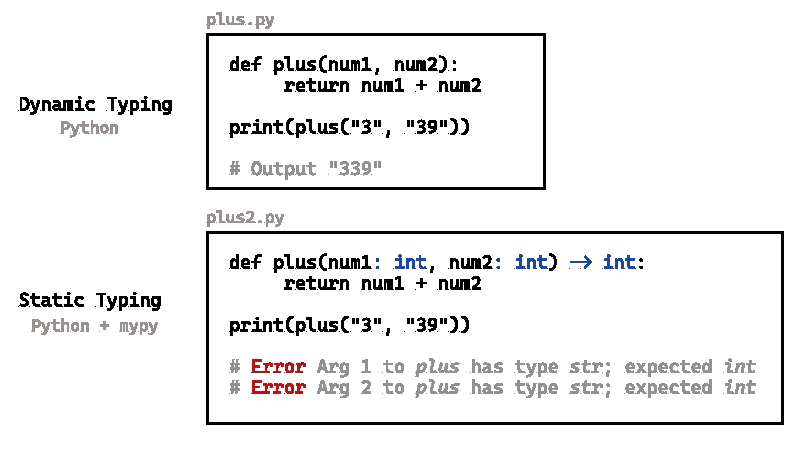
\includegraphics[width=\linewidth]{TypedVsUntyped.pdf}
  \caption{
    \label{fig:typed-vs-untyped}
    Comparison of the same program dynamically typed in Python (Top) and with mypy—a static typing tool for Python (Bottom).  The dynamic-typing rules of the Python interpreter allow it, at run-time, to apply the string concatenating version of the `+' operator -- regardless of the programmer's intention.  By contrast, mypy static-typing checks the type of the values passed to the {\tt plus} function against the intention declared by the programmer through the type annotations on the function parameters (both {\tt int}) and its return type (also {\tt int}).  The type check will fail until the programmer ammends the function call with numeric arguments or otherwise explicitly converts the values from {\tt str} to {\tt int}.
    }
\end{figure}



\section{Functional Programming}

Alongside static typing, \textbf{functional programming} represents another rigorous approach to software development, drawing inspiration from Alonzo Church's lambda calculus in the 1930s \cite{Church1985-bx}. Functional programming treats functions as fundamental building blocks, emphasizing the composition of functions to develop abstractions.

Pure functional programming languages, characterized by immutable values and referential transparency, promote mathematical rigor. Immutable values ensure that once a value is declared, it cannot be altered. Referential transparency guarantees that functions will always produce the same output for identical inputs, providing predictable and testable code.

 A specific subset of functional programming languages, known as `pure' functional programming languages, incorporates additional mathematical rigor through concepts such as immutable values and referential transparency. Immutable values are those that, once declared, cannot be altered. Referential transparency ensures that functions consistently produce the same output for the same input. These properties help mitigate undesirable programming behaviors similar to the way static typing does. For example, the absence of mutable pointers and shared memory in pure functional languages eliminates common concurrency issues like misaligned pointers and race conditions. Consequently, programs developed using these languages are more predictable and can be robustly tested and reasoned about. This significantly reduces the risks that external factors such as network fluctuations or time variations could unpredictably affect program behavior.

Functional programming is often advocated as an excellent choice for introductory programming courses due to its emphasis on mathematical reasoning and strict programming discipline. This discipline includes the clear separation of data from its transformations, fostering a structured approach to problem-solving.


\begin{figure}[hbt]
  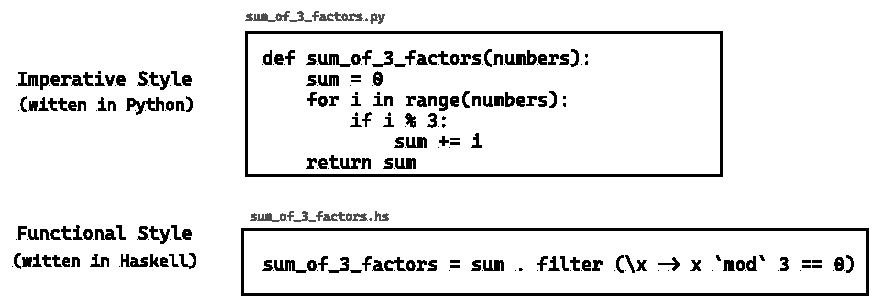
\includegraphics[width=\linewidth]{ImperativeFunctional}
  \caption{
    \label{fig:imperative-vs-functional}
   The same task of summing the factors of 3 in the given numbers, written in imperative style (Top) and functional style (Bottom).
    }
\end{figure}


Functional programming contrasts with other mainstream paradigms like object-oriented programming, which structures programs around objects combining data and behavior, and procedural programming, which focuses on a sequence of procedural steps. Despite the strengths of functional programming, object-oriented and procedural paradigms, exemplified by Java and C, respectively, remain more prevalent in commercial environments. These paradigms benefit from extensive legacy codebases, broad third-party library support, and robust tooling, and familiarity. Lastly, the strictness in functional programming languages may raise the barrier to entry for beginners. For example, in many pure function languages, printing to the terminal window, generally considered a basic technique to observe the execution of the program, requires programmers to understand deep and slightly off-putting concepts like monad and side effects.  


\section{Statically-Typed Functional Languages, The Best Of Both Worlds}
Combining the disciplines described above, \textbf{statically-typed functional languages} employ both static typing and the principles of functional programming. The most common statically-typed functional languages include Haskell,  ML (with the OCaml dialect being the most popular among the family of ML languages), and F\#. 
Of these, Haskell is the only ``pure'' functional language - with all variables being immutable by default.
Descendents of Haskell, like Idris and Agda, include more advanced type-level features like dependent type and session type, allowing programmers to express extremely granular checks of potential software behavior before running the program. These languages often provide the strongest level of programming safety. It is often advertised that programs in these languages will be error-free if the source code passes the compiling stage, indicating that compilers are able to weed out a large number of programming errors. These safety properties allow statically-typed functional languages to be used as proof assistants or formal verification tools. They prove the correctness (or incorrectness) of many systems, from web public key infrastructure \cite{Bhargavan2021-no} to microcontrollers used in space programs \cite{Mokhov2019-zj}. 

Despite these safety benefits, these languages' presence in the mainstream programming world remains underwhelming. This modest popularity is often attributed to high entry barriers, unfamiliarity with the paradigms, and strict type systems that can be daunting for newcomers.

\section{Symptoms of Bad Type Errors}

\ref{sec:symptoms}
 The compiler is the medium through which programmers transform human intention into machine instructions. When encountering errors, compilers often act like Oracles in ancient history, revealing to programmers obscure messages that often lead to huge confusion and a wrong course of action. Many studies have investigated the ineffectiveness of compiler error messages \cite{Barik2017-gy, Becker2019-cs, Becker2016-kc}.  Our exploration is centered around the Haskell programming language and its leading compiler, Glasgow Haskell Compiler (GHC), with the aim of enhancing its handling of type error notifications. It is vital to mention that the challenges discussed here, concerning error messages, are common across compilers for various statically-typed languages. Below, we delve into specific issues often observed in type error messages.


 \subsection{Bias in Type Errors} 
 \label{subsec:bias}
 
A significant issue in type error messages is their inherent bias. Often, type errors can arise from multiple causes, but the error message might only highlight one. This issue is known as left-to-right bias in traditional type-checking algorithms—a notable shortcoming that limits the usability of error messages \cite{McAdam2002-vb, Lee1998-fx, Chen2014-ev}. We will explore this further in Chapter \ref{chap:haskell-type-checking}. For instance, as shown in Figure \ref{fig:type-error-example}, a programmer likely intended to add two numbers using the \texttt{+} operator instead of mistakenly using the concatenation operator \texttt{++}. However, the type error issued by the compiler mistakenly points to the application of the integer literal \texttt{3}, failing to suggest the probable misuse of operators.

 \begin{figure}[hbt]
  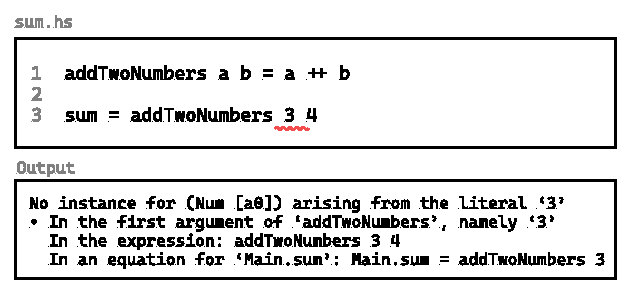
\includegraphics[width=\linewidth]{TypeErrorExample}
  \caption{
    \label{fig:type-error-example}
    Misuse of the concatenation operator \texttt{++} instead of the addition operator \texttt{+} on line 1 is indicated. However, the compiler incorrectly suggests an error due to the use of the integer \texttt{3}.
    }
\end{figure}


\subsection{Type Error Suggests Incomplete Cause}
\label{subsec:imcomplete}

Often, type error messages do not fully present all the locations relevant to the type error. Addressing the error at the highlighted location might not suffice to resolve the underlying problem. Consider the scenario in Figure \ref{fig:type-error-example-2}, where a function intended for list concatenation is erroneously applied to integer values. Here, the error message only reports the first argument, neglecting the second. This partial reporting leads to a situation where correcting the first integer to a list format, \texttt{[3]}, doesn't rectify the error; rather, it only updates to a slightly different error message. 



\begin{figure}[hbt]
  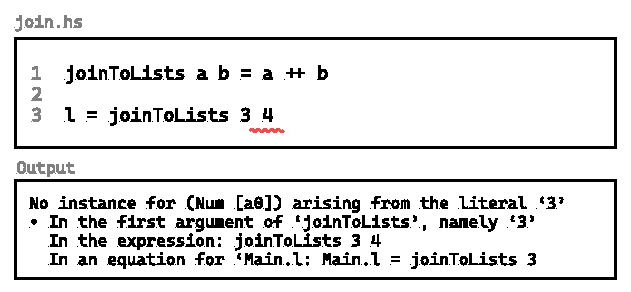
\includegraphics[width=\linewidth]{TypeErrorExample2}
  \caption{
    \label{fig:type-error-example-2}
    A programmer’s attempt to use a concatenation function on integers results in an incomplete error message that only flags the first offending argument. Modifying one argument alone is insufficient to clear the error.
    }
\end{figure}

\subsection{Missing Links In Type Errors}
\label{subsec:missing-link}

One of the most frustrating aspects of type errors is that they do not show the complete pathway of how the compiler decided on the type error. In the example in Fig \ref{fig:type-error-example-3}, the programmer may intend to compare to a char literal \texttt{' '} instead of string literal \texttt{" "}. However, there are multiple clues that contribute to this conclusion: the definition of the function \texttt{trimWhiteSpace}, the application of \texttt{filter isSpace a}, the definition of \texttt{isSpace}, and even the type signature of \texttt{filter} are all needed to understand the logical reasoning. However, none of these are included in the actual error message.


\begin{figure}[hbt]
  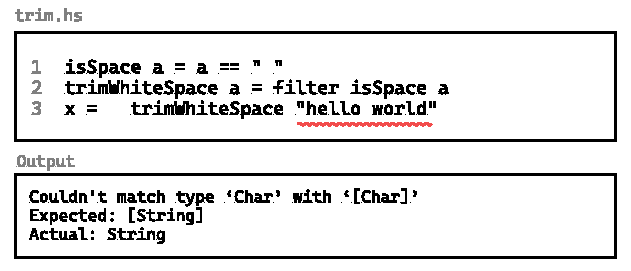
\includegraphics[width=\linewidth]{TypeErrorExample3}
  \caption{
    \label{fig:type-error-example-3}
  This example illustrates how the programmer may intend to compare to a char literal \texttt{' '} instead of a string literal \texttt{" "}; however, the type error ignores all the important clues of how this error is inferred. 
    }
\end{figure}


\subsection{The Use of Obscure Language}

Error messages are frequently plagued by technical jargon and convoluted phrasing, which can be particularly daunting for novices. An example is the error message, \texttt{No instance for (Num a) arising from the literal `3'}, which is an inept way of suggesting a type mismatch involving character and numeric types. In fact, this is often the common behavior across many programming languages and has been shown in many studies \cite{Barik2017-gy, Tirronen2015-nr, Prather2017-dg}. Thus, concerted efforts \cite{Becker2016-kc, Barik2014-ib}  show that rephrasing the error message to be clearer and more structured positively affects programmers' ability to solve these errors.


\section{The Challenges Of Making Good Type Errors}

After introducing some typical symptoms of bad type error messages, we will now explore some fundamental challenges that underpin these symptoms.

\subsection{Types Are Complex}

The advantages of statically typed languages derive from their robust type-checking systems, which, ironically, also introduce significant complexities. Language and tool designers frequently overlook the intrinsic complexity of type systems. In languages that support dependent types, types have the same computing capabilities as runtime programs. This complexity is not limited to dependently typed languages; for instance, type checking in common languages can exhibit Turing-complete characteristics, which might lead to non-terminating processes~\cite{Wells1999-ob}. TypeScript introduces `conditional types', a feature that allows sophisticated computations at the type level \cite{fig:ts-conditional}, posing challenges in explaining errors when these type-level computations fail due to a lack of adequate debugging tools.



\begin{figure}[hbt]
  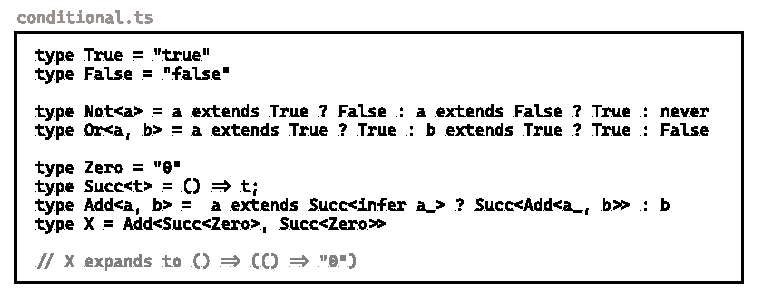
\includegraphics[width=\linewidth]{Conditional}
  \caption{
    \label{fig:ts-conditional}
  TypeScript's feature of conditional types, allows for complex logical conditions at the type level, which can be as complex as the program it annotates.
    }
\end{figure}

\subsection{Clues For Type Checking May Be Implicit}

The task of understanding how types are assigned in a program grows notably more complex when the programming language employs type inference. Type inference \cite{Damas1982-sc} is a technique that allows programmers to forgo the task of writing type annotations. Instead, the type checker automatically deduces the appropriate types for each expression based on the context. Although it succeeded in providing rigorous type checking without the hassle of manually writing type annotations, type inference has been shown to bring many usability issues \cite{Jun2002-xp, Wand1986-lu} for its implicitness.  

Even in programming languages that do not utilize implicit typing, certain typing rules remain opaque to programmers. For instance, rules on permissible values for equality check using the \texttt{==} operator vary across programming languages; some languages disallow comparison of lists, and others are fine with lists but disallow comparison of floating-point numbers. In languages that support a record data type, programmers must navigate additional complexities, such as whether adding or removing a field from a record maintains type correctness \cite{fig:row-polymophism}. This often involves an understanding of nuanced language-specific rules, including concepts like covariance, contravariance, and subsumption.


\begin{figure}[hbt]
  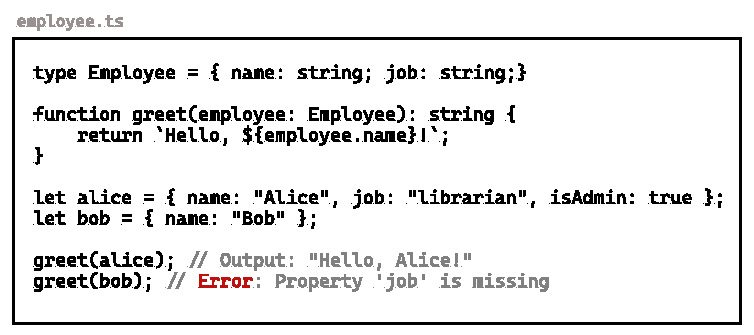
\includegraphics[width=\linewidth]{RowPolymorphism.pdf}
  \caption{
    \label{fig:row-polymophism}
Row polymorphism enhances flexibility in structuring data collections but also introduces complexity in understanding type substitutions and variance.
    }
\end{figure}

These challenges amplify the difficulty in designing intuitive type error messages. The complexity of type systems demands that designers have a profound understanding of both theoretical and practical aspects of language implementation—knowledge often possessed only by the core language developers. Moreover, the implicit nature of modern programming languages requires that type errors be designed on a case-by-case basis, a daunting task given the limited number of contributors who possess the necessary expertise.

\section{The Lack of Type Debugging Tools}

Debugging programming errors has been an unpleasant but crucial part of programming since the inception of computing, tracing back to as early as 1949 \cite{Campbell-Kelly1992-rn}. However, the tools and support for debugging type errors have not evolved significantly and do not match the advancement of those available for runtime errors.

One of the simplest and most dependable debugging techniques is to insert \texttt{print} statements. As computing pioneer Brian W. Kernighan once noted, ``The most effective debugging tool is careful thought, coupled with judiciously placed print statements'' \cite{Kernighan1978-xs}. Furthermore, breakpoint debugging has become a staple in nearly all programming Integrated Development Environments (IDEs), allowing for intermittent code execution and inspection \cite{fig:breakpoint}. Research in error debugging tools continues to be dynamic. For instance, ZStep94 \cite{Lieberman1995-lg} enhances traditional breakpoint debugging by eliminating the need to set breakpoints, thus enabling programmers to view and navigate through the historical values that expressions take throughout execution (Figure \ref{fig:zstep94}). Another innovative tool, WhyLine \cite{Ko2009-uf}, aligns with the principles of a natural programming environment \cite{Myers2004-fy} by allowing programmers to ask ``why'' questions and ``why not'' questions about certain program behavior.

Despite these advancements in runtime debugging tools, the development of type debugging seems to have stagnated. Most programming languages and development environments still handle type errors in ways reminiscent of early languages like FORTRAN and ALGOL. In recent years, some modern programming languages like Elm and Rust have made efforts to improve type error reporting, but these enhancements are often superficial and do not fundamentally change the debugging experience.


\begin{figure}[hbt]
  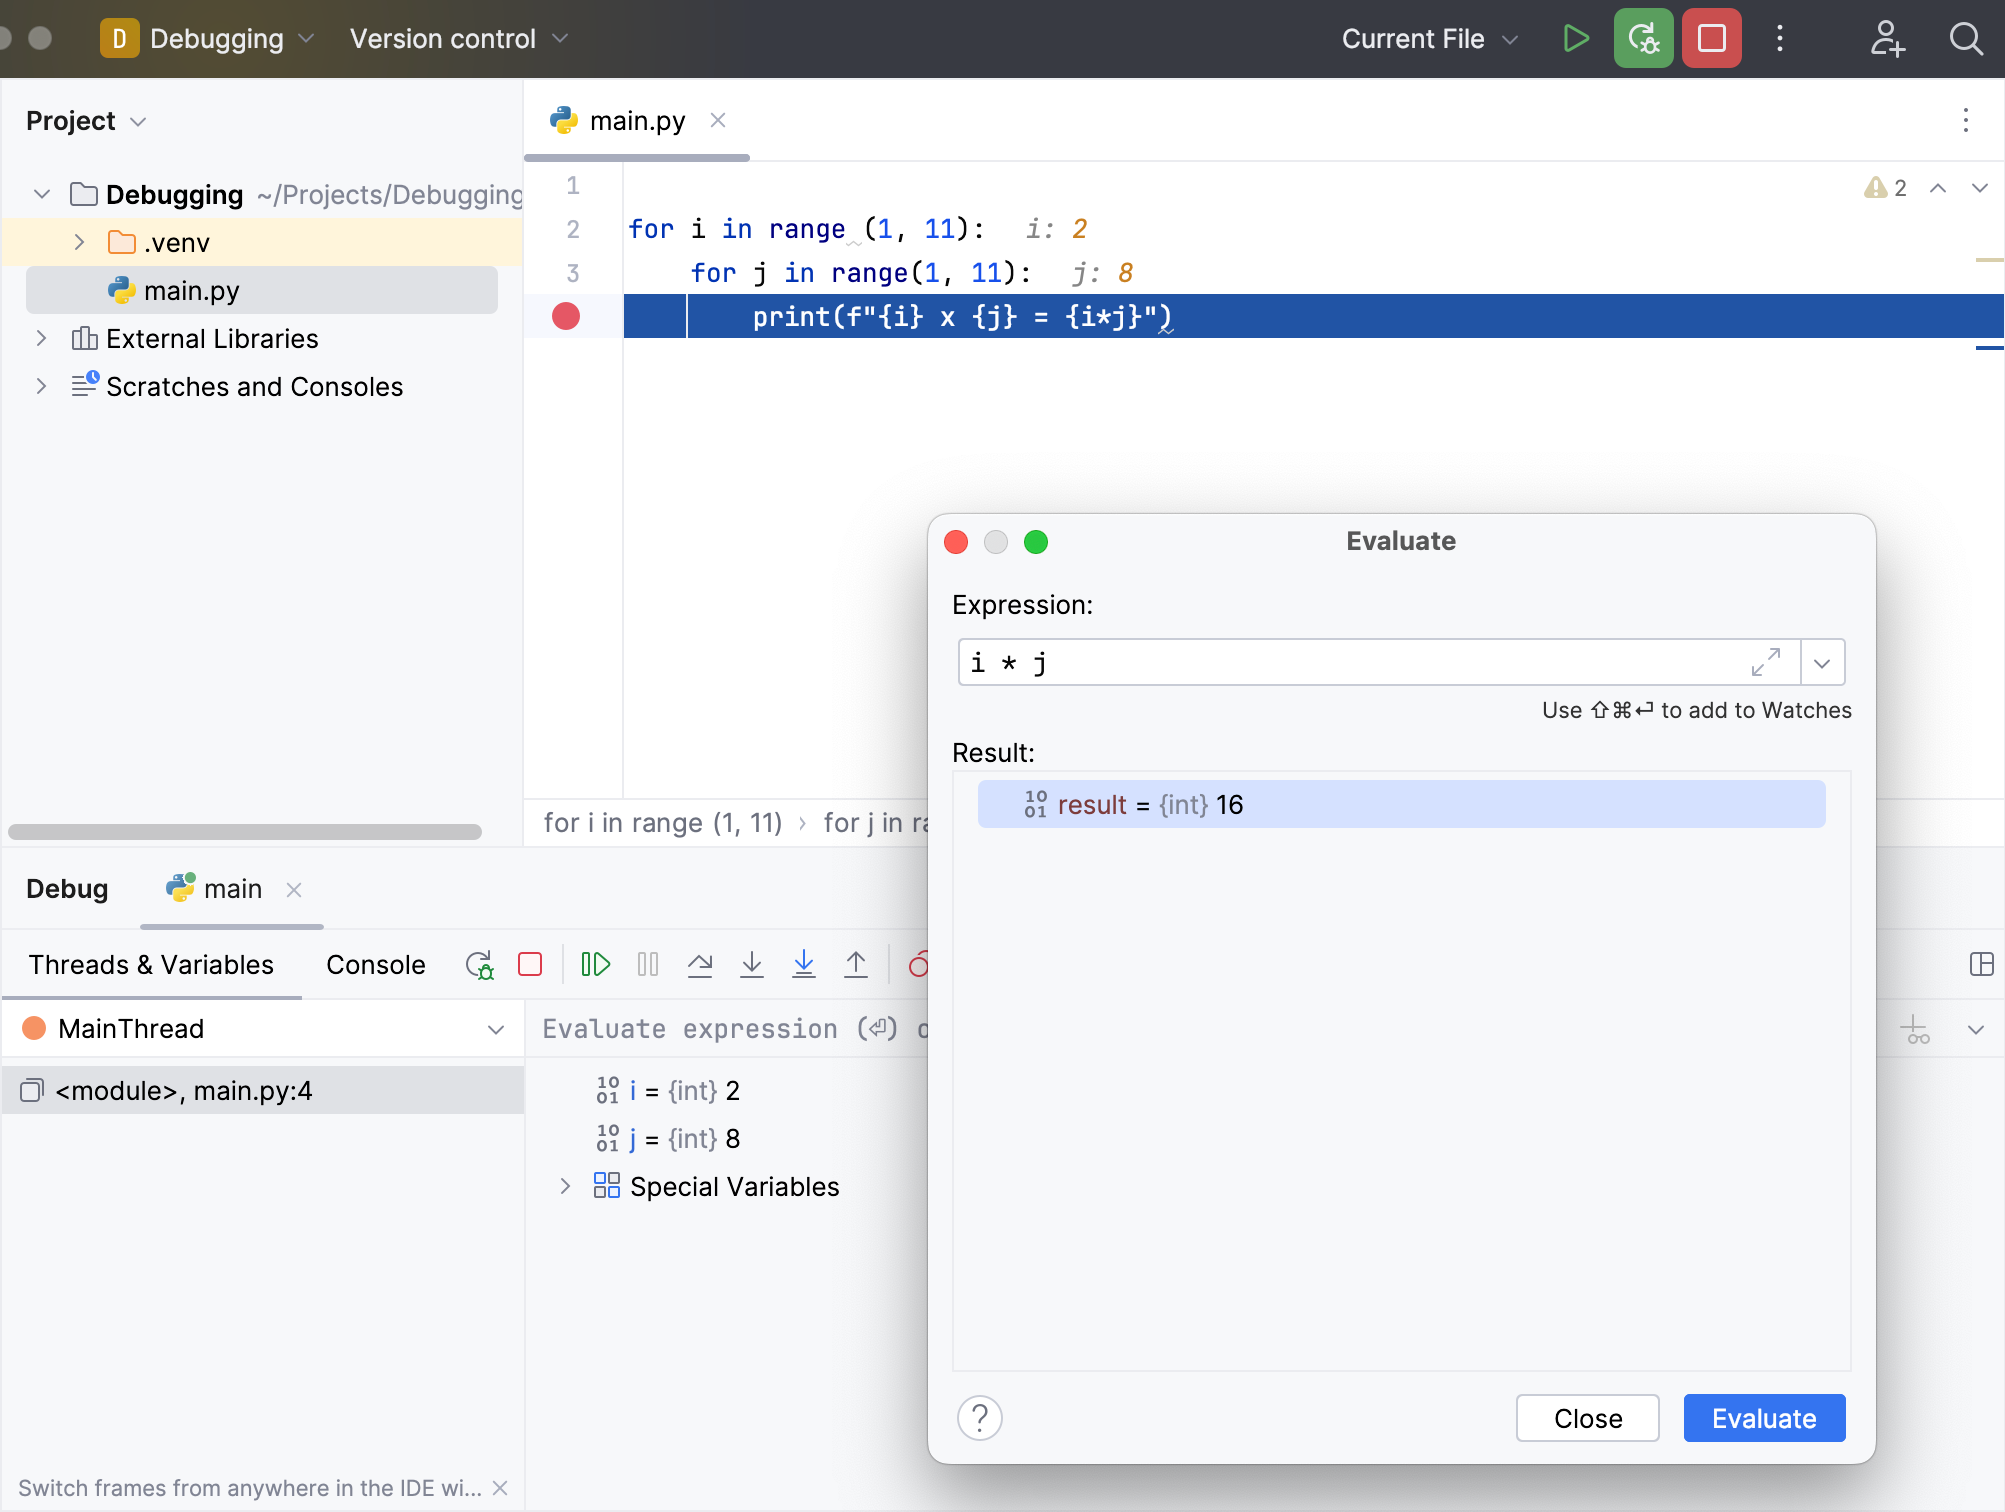
\includegraphics[width=\linewidth]{BreakPoint}
  \caption{
    \label{fig:breakpoint}
    Debugging a Python program using a breakpoint debugger and expression evaluation in PyCharm.
    }
\end{figure}


\begin{figure}[hbt]
  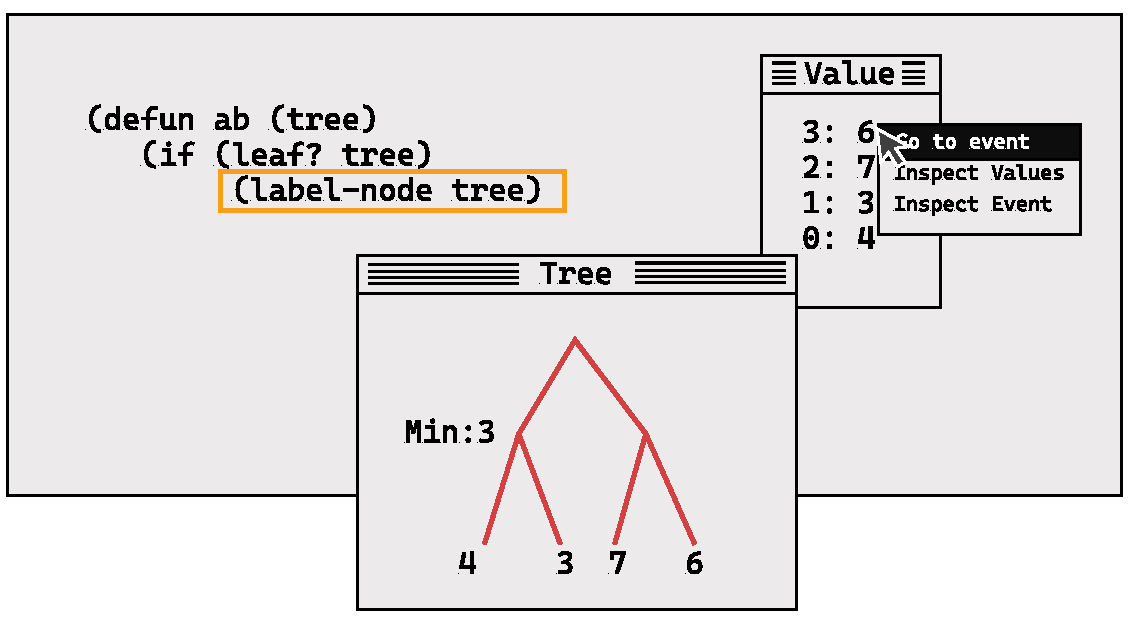
\includegraphics[width=\linewidth]{ZStep94}
  \caption{
    \label{fig:zstep94}
    Debugging a Lisp program by inspecting all the historical values of an expression, navigating through execution history, and reviewing live visualization replay.  All these features are provided in ZStep94.
    }
\end{figure}

My research is driven by the acknowledged difficulties in debugging type errors and the lack of significant advancement in the interfaces and techniques used for presenting and resolving these errors through modern graphical user interfaces and human-computer interaction techniques. This area holds considerable potential for improving both the usability and accessibility of statically typed languages, making them more approachable for developers at all levels of expertise.

\section{Research Aim}

\subsection{Aim 1. Provide Programmers With The Comprehensive Knowledge Needed to Understand and Resolve Type Errors.}
\label{subsec:aim1}

Current representations of type errors in most compiler tools are often insufficient, typically providing only the location of the type check failure, the expected type, and the actual type encountered. This conventional approach, as discussed in the previous sections (\ref{sec:symptoms}), lacks practicality and clarity. This aim addresses the need for a richer, more informative explanation of type errors by evaluating the limitations of existing systems and analyzing how programmers tackle type errors in practice.

\subsubsection{Objective 1.1 To Encompass Multiple Potential Causes Of A Type Error}
An essential aspect of this research is to challenge and expand beyond the bias found in traditional type error reporting (Section \ref{subsec:bias}). It's crucial to inform programmers of multiple potential causes and resolutions. A key goal is to communicate these multiple dimensions effectively. In addition, for each potential cause, programmers need a clear explanation of where the offending code is, which typing rules are violated, and how the type might change after the error is resolved.


\subsubsection{Objective 1.2 To Accurately Report Relevant Locations Contributing to Type Errors.}
Current tools often pinpoint a single location for a type error, a method that has attracted considerable criticism for its inefficiency. Programmers frequently need to scan beyond the initially reported location. This research aims to enhance type error reporting by identifying and detailing all relevant error-contributing locations across the codebase.

\subsubsection{Objective 1.3 To Give Reasons And Support Human Understanding}
Understanding type errors goes beyond pinpointing the location in the code. Internally, type errors can be caused by mismatched types, unmatched type class constraints, or trying to construct infinite types. Externally, type errors can be caused by typos, outdated type annotation, incomplete implementation, etc. Our goal is to not only find these errors but to explain them in a way that logically supports the programmer's understanding and troubleshooting process, covering both internal causes and external causes.



\subsection{Aim 2. Support Programmers To Type Errors Through Interactive Modern Programming Environments.}

This aim focuses on integrating comprehensive type error encoding (Section \ref{subsec:aim1}) within an interactive programming environment to streamline workflows in statically typed languages. It acknowledges that an increase in information does not necessarily correlate with enhanced understanding and aims to present type error details in a way that optimally supports comprehension and resolution.

\subsubsection{Objective 2.1 Visualize The Key Concepts Of Type Errors Effectively}

Traditional text-based error reports can be difficult to navigate and understand. This objective explores innovative methods to present what used to be displayed as plain text (type signatures, locations in source code, call stacks, dependency graphs) in a novel and intuitive way. Examples include in-line highlighting within the code editor and graph-based reasoning steps.  

\subsubsection{Objective 2.2 Use Interactive Tools for Investigating and Resolving Type Errors.}

This research will explore interactive techniques to dissect and explore type errors in a manageable and meaningful way. By breaking down errors into smaller, understandable units, programmers can methodically trace and address the root causes. This includes providing context-sensitive debugging aids that adjust the level of detail presented based on the error type and individual user preferences, ensuring a tailored and effective debugging experience.


\section{Contributions}

\subsection{A categorization of type errors based on the structure of the evidence of a type error}

To address the complexities in explaining type errors comprehensively, we have classified type errors into three complexity categories based on a human perspective. Formal definitions and a detailed discussion of these categories appear in Chapter \ref{chap:haskell-type-checking}. It is crucial to understand that these categories are not mutually exclusive; for example, a multi-witness type error may also be a multi-step type error.


A \textbf{multi-step type error} occurs through a chain of logical inferences steps based on the available evidence of the error. Figure \ref{fig:multi-step-example}) illustrates the chains of inference in the assignment of a (Line 1), the equivalence of a (Line 1 and Line 2), the assignment of b (Line 2), and the equivalence of b (Line 2 and Line 3). Removing any one of the chains will resolve the conflict. Understanding and communicating the interconnections within these chains is crucial to resolving multi-step type errors effectively.

\begin{figure}[hbt]
  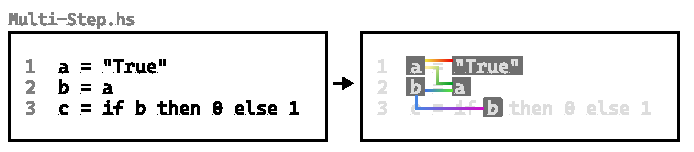
\includegraphics[width=\linewidth]{Multi-Step}
  \caption{
    \label{fig:multi-step-example}
    Illustration of a multi-step type error in Haskell.  The potential issues in the definition of \texttt{a}, \texttt{b}, or the conditional expression of variable \texttt{b}. It can be clearly seen a ``chain'' of reasoning formed in order to explain the type error. }
\end{figure}

A \textbf{multi-witness type error} entails multiple pieces of evidence supporting the same potential type assignments. For instance, as shown in Figure \ref{fig:multi-witness-example}, multiple evidence (lines 3,4,5) support that a has the type \texttt{Int -> String}. On the other hand, a single piece of evidence (line 2) shows that a has the type \texttt{Int -> Char}.  Clarifying and juxtaposing this discrepancy in witnesses is key to supporting understanding this type of error.

\begin{figure}[hbt]
  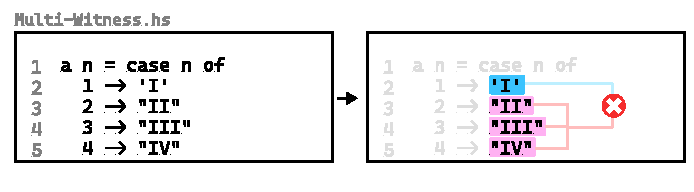
\includegraphics[width=\linewidth]{Multi-Witness}
  \caption{
    \label{fig:multi-witness-example}
    Analysis of a multi-witness type error, where the \texttt{case} expression could be interpreted as type \texttt{Char} or \texttt{String}. This scenario showcases a type disagreement with witnesses (in color pink) against one witness (in color blue). It is not hard to see that the difference in number play an important role here as the char literal \texttt{'I'} on line 2 is more likely be a typo.
    }
\end{figure}

A \textbf{multi-party type error} involves several potential type assignments, each supported by distinct evidence.  Figure \ref{fig:multi-party-example} presents a typical multi-step type error: the expression \texttt{d} can not be assigned a type because 3 pieces of evidence on line 1 suggest 3 potential types for \texttt{d}. In practice, addressing such errors requires decomposing them into multiple type errors of simpler forms.


\begin{figure}[hbt]
  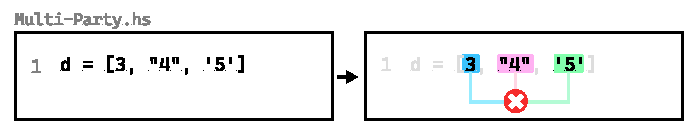
\includegraphics[width=\linewidth]{Multi-Party}
  \caption{
    \label{fig:multi-party-example}
    Analysis of a multi-party type error regarding the list \texttt{d}, which could alternately be typed as \texttt{[Int]}, \texttt{[String]}, or \texttt{[Char]}. The conflict is depicted as a disagreement among three parties (Right). Unlike the previous two examples, this error cannot be fixed by a single location. }
\end{figure}

These classifications have led to the development of three distinct systems—Chameleon, Goanna, and GeckoGraph—each designed to tackle unique challenges within the domain of type error debugging.

\subsection{Explaining Multi-Step Type Errors Through Chain-Of-Thought Visualization}

\subsubsection{Technical Contribution - Chameleon}


We contribute Chameleon, an interactive Haskell debugging tool that not only identifies all relevant error-contributing locations but also illustrates the logical relationships between these locations. Chameleon provides a novel debugging interface to interactively explore the chain of reasoning in a multiple-step type error, allowing programmers to develop a panorama view of the type error interactively. In addition, Chameleon uses an adaptive interface design; programmers can switch between different granularity of information based on their personal preferences. 

\subsubsection{The evaluation on the effect of error slicing and chain of thought visualizations}
We evaluate the efficacy of interactive visual debugging tools in contrast to conventional type error debugging methods. We have conducted studies that assess how programmers resolve type errors using various interfaces ranging from basic type error slicing techniques to Chameleon's step-wise interactive debugging tools. These evaluations aim to measure how enhancements in the debugging process can influence error resolution tasks' efficiency and intuitiveness.

\subsection{Iterate potential causes of multi-witness and multi-party errors}

\subsubsection{Technical Contribution -- Goanna}
Goanna enhances type error debugging in Haskell by not only identifying all relevant error-contributing locations but also dividing the type error into possible causes and their respective resolutions. It ranks these potential causes based on their likelihood, helping programmers systematically approach error resolution.

\subsubsection{An evaluation on accuracy, conciseness, and performance of MCS-based type debugging and our heuristics}
We evaluated Goanna's performance across a diverse set of Haskell programs, analyzing its accuracy and performance in error identification against traditional tools. We evaluate Goanna's conciseness in narrowing down potential causes into a shortlist. 


\subsection{Visualizing Types}

\subsubsection{Technical Contribution -- GeckoGraph}

We contribute GeckoGraph, a graphic notation for Haskell types. GeckoGraph encodes the same information as type signatures but uses colors, shapes, and symbols to make certain structures easy to identify at a glance. GeckoGraph uses visual elements to improve the understanding of complex type concepts, such as type classes and qualified constraints. GeckoGraph offers clarity when reading dense type signatures and comparing multiple types.

\subsubsection{An evaluation on how programmers use graphic type notation}

We contribute a large-scale empirical study exploring the effectiveness of graphical type representations like GeckoGraph in enhancing programmers' abilities to tackle type-related tasks.

% \section{Research Method}

% \subsection{Human-centered programming language studies}

% One important decision that shape a lot of my work is employing human-centered research methods with our novel programming language systems. The adopting of human-centered methods happens at every stage of the projects: prototyping, development and evaluation. Although the using of these methods are not new at all, but they certainly are not the most polular choices in programming language studies.

% The motive of such decision is that it is impossible to understand what are the good qualities of type errors without observing how human use type errors to gain understanding. 


% The downside of study programming language is iterative design is very hard. programming tasks involves complex inputs and outputs, and it is very hard to study an incomplete system without a fully working systems. For instance, if we are to study the effect of type errors, it is most effective to have a system that can recognize type-correct program from ill-typed one. It is hard to evaluate with a mock-up or wizard of oz style fake outputs to study users' interaction.  To address this limitations, we have a few ideas implemented in our research:

% A minimal but practical set of language 
% Design for human from start



\section{Thesis outline}

 This thesis is structured into two main parts. The initial chapters build a comprehensive foundation on type systems and programming languages, setting the stage for my research contribution in subsequent chapters. The latter chapters focus on distinct contributions that tackle various challenges in type error debugging.

\subsection{Chapter 1}
Chapter 1 sets the stage by discussing the fundamental concepts of programming languages and type systems. It explores the trade-off between enhancing program safety and optimizing usability, a central dilemma in programming language research and software engineering practice. The chapter highlights common issues and technical challenges associated with type errors, establishing the motivation for this research. It also outlines the specific aims and contributions of the study, providing a clear roadmap for the thesis.

\subsection{Chapter 2}
This chapter delves into the fundamental concepts underlying type systems and programming languages. It outlines traditional methods employed in Haskell type checking, error slicing, and interactive debugging. Additionally, this chapter discusses tools and techniques used in constraint satisfiability analysis that are integral to later developments in the thesis. The categorization of type errors is revisited and redefined, building on the definitions introduced in this chapter.
    
\subsection{Chapter 3}
Chapter 3 presents Chameleon, a system designed to enhance the debugging of type errors through interactive visualizations. It begins with a discussion on the typical pitfalls of existing error messages and outlines the motivation behind Chameleon. We then detail the system's design, features, and development process, including iterative prototyping. A series of empirical studies were conducted to assess Chameleon's effectiveness compared to traditional compiler tools.
    
\subsection{Chapter 4}
Chapter 4 introduces Goanna, a Haskell type error debugging tool that incorporates novel features such as suggesting fixes for type errors and cross-module debugging capabilities. It starts with highlighting the limitations of conventional compiler error messages and progresses to describe Goanna's capabilities in identifying all causes and ranking potential causes by their likelihood. The implementation tactics and heuristic methods used in Goanna are discussed, followed by an empirical evaluation of the system's accuracy, conciseness, and performance based on real-world Haskell code examples.
    
\subsection{Chapter 5: GeckoGraph — Visualizing Haskell Types}
The final chapter synthesizes the thesis's contributions and situates them within the broader research context. It discusses potential avenues for future tool development and research opportunities, forecasting the future landscape of research in type error improvement. The chapter concludes with reflections on the expansive and still largely unexplored territories in programming languages, encouraging ongoing investigation and innovation.

    
\subsection{Chapter 6: Conclusion}
The final chapter synthesizes the thesis's contributions and situates them within the broader research context. It discusses potential avenues for future tool development and research opportunities, forecasting the future landscape of programming language research. The chapter concludes with reflections on the expansive and still largely unexplored territories in programming languages, encouraging ongoing investigation and innovation.


% Chapter 2

\chapter{Background}
\label{chap:background} 

Programming in strongly typed languages has many advantages. It helps programmers identify logical errors before running the code, reduce maintenance difficulty, and improve the editor capability find documents and auto-complete code while typing. However, the difficulties in understanding and resolving type errors often ward people off  from practicing strongly typing.  In this Chapter, we discuss the relevant research in improving the experience of debugging type errors. We first investigate the theoretical approaches to enrich/correct the information presented type errors. We then  investigate the various designs of tools, interfaces, and visualizations to support understanding type errors.

\graphicspath{{Figures/Background}}


\section{Functional Programming}

Functional programming is a programming paradigm that treats computation as the evaluation of mathematical functions and avoids changing state and mutable data. The roots of functional programming are deeply embedded in mathematics, stemming from the lambda calculus - a mathematical system built around function abstraction and application - developed by Alonzo Church in the 1930s.


The early functional programming languages include Common Lisp in the 1950s, Scheme invented in the 1970s, and ML in the 1970s. In the 80s  the language Miranda was developed, introducing the world to more flexible functional concepts, such as lazy evaluation. However, some of these ideas were commercialised, which spurred the creation of Haskell – a purely functional language produced by the open-source community, later becoming a seminal achievement and most influential functional language in academia and the programming industry.


In the 21st century, although new functional programming languages are continue to be created, such as Clojure, F*, and Idris, what’s more often interesting to see is functional programming ideas and benefits into other paradigms. Scala is a programming language that combines the expressiveness of functional composition and ergonomics of object oriented programming. JavaScript, a traditional multi-paradigm language, started to adopt programming features such as lexical scoping, tail recursion optimization.


In 1978 John Backus delivered his Turing Award lecture, “Can programming be liberated from the von Neumann style?”, bringing functional programming into the recognition in the larger programming world. Different from other paradigms in the programming realm, functional programming brought a few innovations that changed the thinking in the academic and programming community, and has been sought after by other paradigms for decades to come.


\textbf{Declarative}: being close to mathematical functions, functional programs are the composition of forms that map value from one domain to another. Instead of explaining how to achieve a specific task step-by-step (like in imperative languages), functional programming encourages developers to describe what they want to achieve and the language abstracts the how.


\textbf{Immutability}: Unlike object-oriented programming, where data structures (such as objects) could be changed, or mutated, data in functional programming is immutable, meaning it cannot be changed after creation. This trait reduces the chances of bugs because you know that your data isn't changing unexpectedly.


\textbf{Pureness}: pure functions are functions that observe referential transparency, in other words when given the same input will always reach the same output. The pureness of functional programming seems to be a big restriction and handicap on what a function can do, for instance, that pure functions cannot access external systems or produce true random numbers. However, pure functions are as potent as they are limiting, it creates a strong separation between data and programs and powerful transformation can be developed on the premise that no side effects are present in the programs.


\textbf{High order functions}: The idea of using functions as normal values where they can be assigned to names, returned by other functions, or passed as arguments is a fundamental ingredient of functional thinking. This aspect allows programmers to create more abstract functions and reusable logic. Currying is a special case of high order function, where a function with multiple arguments is transformed into a sequence of functions, each with a single argument. Currying is beneficial for creating simpler and cleaner functions and aids in code reusability.

\section{Statically Typed Languages and The Typing Debate}


Static typing has been practised since the very start of programming languages. Fortran, known as the first compiled programming language, has explicit types for integers and floating point numbers, and uses static typing to reject mal-formed programs. Later programming languages Pascal, C were all designed to use static typing. In these languages, user defined types, such as functions and structs, have become available, making the type checking more flexible and reliable.

 
Functional languages, especially Haskell, took the static types further with ideas coming from academic languages, such as typed lambda calculus and system F, that are shown to be sound and complete. Many type-level features in Haskell were later exported to languages of other paradigms.  Polymorphic types were introduced to allow functions types to be defined more fluidly so that they can work with any data types. Type inference (also known as implicit types) was introduced to allow static type checking even without any explicit type annotations. These features can now be found in most mainstream programming languages. (Give an examples of )


Compared to static typing, the alternative typing discipline – dynamic typing – provides many appealing benefits, and has strong influence in the computing world. In dynamically typed languages, a variable can hold different types of values because the type is checked during runtime. This provides more flexibility than static typing since a single variable can be used to hold different types of values through mutation or reassignment. However, it also means that errors such as trying to subtract a string from a number can be detected only when the code is run, leading to potential runtime errors.


The lisp programming languages, such as common lisp and scheme, were designed to benefit from the flexibility of dynamic typing. In Lisp languages, functions often take dynamic input that can be various forms (atom, lists, s-expressions), and different code is executed based on inspecting the input value at runtime. In modern day computing,  languages like JavasScript, Python are all dynamic languages, which is believed to contribute to their immense popularity thanks to the lower barrier of entry.

\subsection{The arguments for static typing}
\textbf{Program safety}: Static typing can catch errors and bugs during compile time, before the software even runs. This can be particularly beneficial when working on large code bases or complex systems.

\textbf{Ease of Maintenance}: Static typing allows common software engineering tasks, such as refactoring code more reliable. In general, a software project will not successfully compile unless all the  locations affected by the initial changes are addressed and resolved.

\textbf{Additional Tooling Support}: The type information in static languages can help programmers understand code better and faster. This is often shown as richer information in documentation, or more detailed pop-over type hints with modern programming IDEs.  

\subsection{The arguments for Dynamic typing}

\textbf{Ease of Use and Flexibility}: Dynamically typed languages usually have a simpler syntax, and the flexibility of being able to change the type of a variable on the fly.

\textbf{Rapid Prototyping}: Dynamic typing can be faster in terms of development, facilitating quick prototyping and scripting.

\textbf{Metaprogramming}: Dynamically typed languages are robust in metaprogramming because they can inspect, generate, and modify code more flexibly during runtime.


\section{The Mission To Improving Type Errors}

Type errors can be notoriously difficult to understand and use, particularly for newcomers to programming or when using a language that is more strict about types. Type errors are often believed to be a major contributor to static typing's popularity. Type errors can happen in dynamic languages as well, however, they are not as difficult as their counterparts in static languages.

Comparing to other programming errors (parsing errors, runtime errors), type errors have some distinct characteristics that render them particularly challenging. 

\textbf{Lack of runtime values}
Types are computed at compile time, and just like the evualting programming sematics, the type checking computations can be complex. In fact, many programming languages type checking are shown to be non-terminating and turing compelte.  Unlike runtime evaluation, type checking cannot be inspected using conventional tools. Inserting print statement inside type annotation is not possible. 

\textbf{Clues for Type Checking are Implicit}
Understanding type assigments of the program become more challenging when the programming language uses implicit typing. Implicit typing, also called type inference, is a technique that allow programmers to omit the ritual of writing type annotations all together and the type checker will infer the most general types (principal types) for each expression. Even for languages that don't employ implicit typing, some typing rules are hidden from programmers.
For example the \texttt{if} expression in many programming languages. The semantics is very clear, but the typing rules are hidden.


\textbf{Lack of tool support}
Lastly, few tools are dedicated on supporting type erros. Runtime programming errors have been studied thouroughly as a research subject and numerous industry tools are focus on understanding and solve runtime errors(GDB, breakpoints, time travel debugger..)  However, in comparason, tool support type error  remain the same depth and capability as they were many decades ago. Most the programming environments render type errors verbatem to the terminal.   


To start, the languages used in type errors are often unhelpful to programmers. On one side, type errors often involve terminology and concepts that can be difficult to understand, particularly for less experienced programmers. The concepts might include objects, instances, classes, functions, variables, or aspects of data types that haven't been encountered before or fully understood. This is exemplified to extremes in Haskell, where programmers are often perplexed by errors like “No instance for (Num Char) arising from the literal '1'”. One another side,  the error messages returned for type errors are either vague or misleading. They might indicate the line of code where the error was detected but the actual mistake might be somewhere else.


Another factor of the difficulty of type errors is the lack of supporting information. Programmers can get stuck in a type error for hours and concede that dynamic languages are easier. When type errors are at runtime, programmers can at least run the program and insert printing statements to observe the dataflow of the program. None of these debugging techniques work on type errors as they are reported without actually running the program.  This is  comparable to debugging parse errors, which also happen at compile time. But generally parse errors are often local, meaning that a parse error has a sensible range of locations,  indentation errors can be searched in the parent indentation block, unmatched brackets can be searched in the outermost brackets. On the other hand, type errors are more global, a type conflict can happen between two different files, or code from different sources. This added to the difficulties of solving type errors.
 

Type errors are made harder with more advanced type system features have been introduced. As a result the usability of type systems decreases as the expressiveness of the type system increases. For example polymorphic types allow types to be defined to restrict the relations between types instead of the types themselves. For example the (==) :: a -> a -> Bool function can be defined to compare two values of the same type, without specifying which type it must be. However, this will add confusion when too many polymorphic variables are participating in the type error and compilers sometimes rename them to further mystify the case.


Throughout history, many have dedicated their research to improving type errors, making them easier to understand and better at helping to find the root causes. We categorise them into three major themes: Enhanced compiler error message, reporting multiple nodes, and interactive debugging.

\subsection{Enhanced Compiler Error Messages}

A well-studied approach to producing better error explanations is through ECEM (Enhanced compiler error message).  As put in~\cite{Barik2017-gy}, ``Error messages appear to take the form of natural language, yet are as difficult to read as source code."   Through a series of mixed-method studies, Prather showed~\cite{Prather2017-dg} that ECEM has a positive result in understanding compiler errors. Decaf~\cite{Becker2016-kc} is a tool that can rephrase Java compiler error messages into an enhanced version. In a study of over 200 CS1 students, Decaf was shown to reduce overall errors in their coding practices. Berik proposed a framework~\cite{Barik2018-xs} for constructing compiler error messages based on argumentation theory, and showed that error messages following a simple argumentation layout or an extended argumentation layout are more human-friendly.  These works show the significance of improving the language in the compiler error messages. 


\subsection{Reporting Multiple Nodes}

\begin{figure}[hbt]
    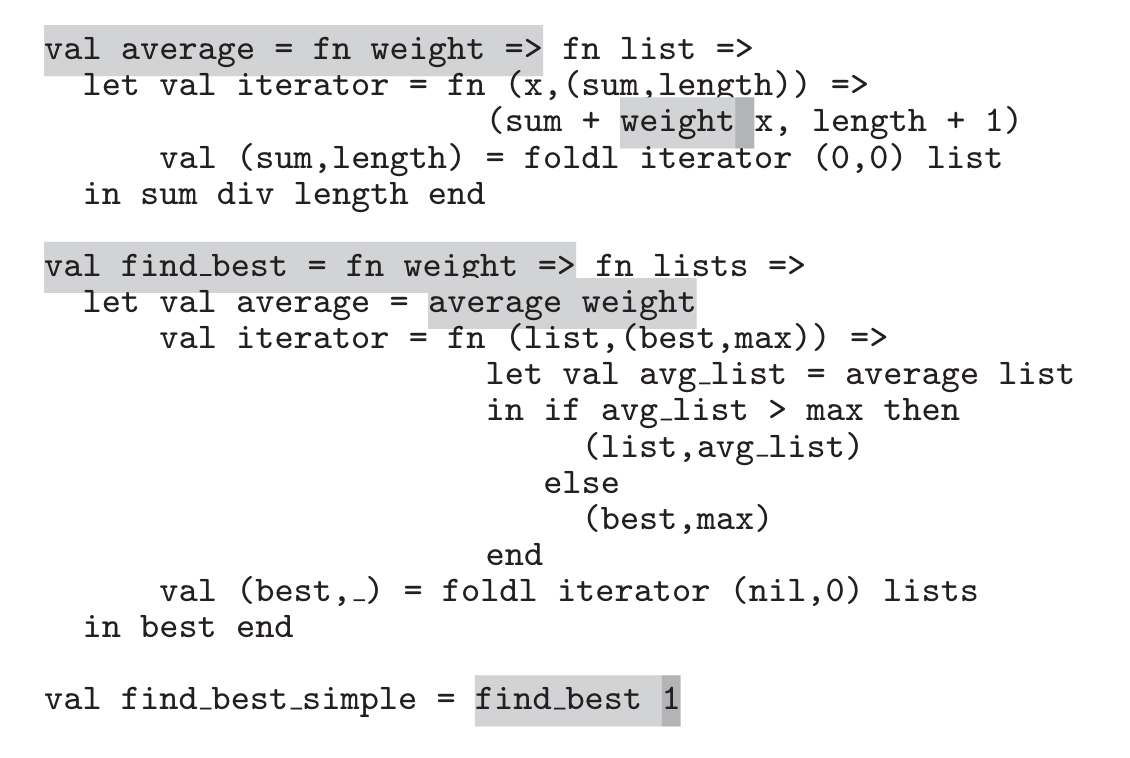
\includegraphics[width=0.6\linewidth]{HaackTypeErrorSlicing}
    \caption{An example of Type Error Slicing by Haack and Wells
    }
\end{figure}

Many have studied the approach of finding all locations that contribute to a type error~\cite{Stuckey2003-pz, Haack2004-fr, Pavlinovic2015-ke, Schilling2012-iq}. Type error slicing~\cite{Haack2004-fr} is a technique that finds locations that are complete and minimal for the type error. Internally labeled constraints and Minimal Unsatisfiable Subset (MUS) generation are used to generate these slices. The language supported in Haack's work was a subset of Standard ML. The original Chameleon~\cite{Stuckey2003-pz} used  Constraint handling rules (CHR) to support the computing of type error slices in Haskell. Chameleon also supported advanced type-level features (type classes and functionally dependent types). The project also introduced the ability to query type information through a command line interface. Although Chameleon was firmly grounded in results from type theory, its designs were never evaluated with user studies. While finding all error locations is useful in comprehending type errors, it is only 1 of the 7 properties listed in the proposed manifesto of good type error reporting~\cite{Yang2000-wn}.

\subsection{Interactive Debugging}

\begin{figure}[hbt]
    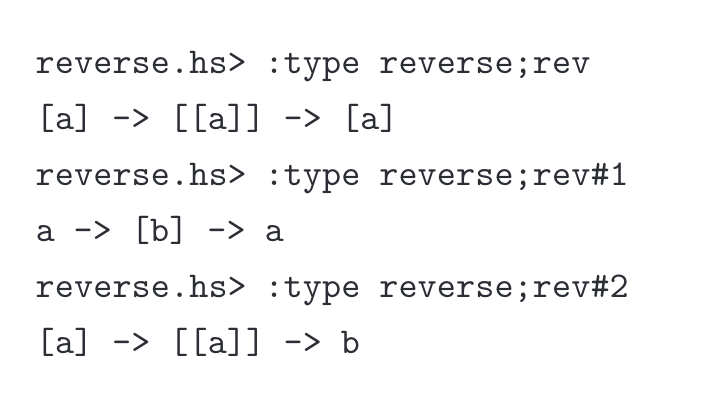
\includegraphics[width=0.6\linewidth]{ChameleonInteractive}
    \caption{An example of Type Error Slicing by Haack and Wells
    }
\end{figure}
Interactive debugging is a method in which programmers can selectively view the debugging information, test and retract their assumptions, and  make changes and observe their effects. Interactive debuggings have been practised for a long time for debugging runtime errors. Programmers often use techniques such as pause/break (also known as a breakpoint) a running program, inspect the current state, and change values if needed. It's highly beneficial because it allows the programmer to interact with the program at runtime, which can provide valuable insights into the state of the program and help identify errors. However, for type errors, programmers are stuck with static error messages in text form. However some early ideas of interactive debugging were proposed in research. Chameleon is an Haskell interactive type debugger that works in command line interface. When encountering a type error, Chameleon is able to analyse and deduce alternative ways a type error can be fixed, and programers can select an alternative they desire by typing in command.


\section{Verify Generated Source Code -- a case for the future}

One trend we have seen in recent years is that generative AI models are widely used to generate code. Once trained, these models can generate code snippets or complete applications based on user input. This might take the form of a natural language prompt, a framework or blueprint layout of the needed application, or even a sequence of tasks or features the code is intended to address. Many models trained in large corpus of software projects show competence in producing source code according to human prompts. However, it seems inevitable that source code generated by a large language model may contain errors, undesired behaviours, or even critical security vulnerabilities. Another big concern is that it is hard to get a grip of the accuracy of AI generated code with popular metrics. In this, human evaluation is still significantly better than automated metrics.


 We believe that statically typed functional languages are the ideal candidates for code generations of these tools. The functional requirements force the pure functions and effect to be clearly separated, where undesired behaviours, such as making database connections, or sending network packets to an external party, are harder to sneak in. In addition, the static typing forces that the generated code must be conformative to the specification. And thus, we strongly believe that now more than ever, we need intuitive type error messages, and streamlined type error debugging processes, to accommodate traditional human written programs, and to tame the AI generated code.


 \section{Conclusion}
 In this chapter, we followed the footsteps of the historical development of functional programming languages and statically typed languages, and their current status in academia and the programming industry. We showed through multiple studies where there is a lack of attention in the design of type errors. We explored multiple research projects that were dedicated to improving the type errors and the way programmers debugging them. We also took a peek at the potential future of programming, and how our effort in improving type errors may help brighten such a future. 
% Chapter 3
\newcommand{\chameleon}{Chameleon}

\chapter{Chameleon: An MUS-based interactive type error visualization and explanation tool}
\label{chap:chameleon:design} 


Dynamically typed programming languages such as JavaScript and Python have risen in popularity in recent decades \cite{chatley_next_2019}. These languages present a low barrier of entry, especially to beginner programmers: they require no type declaration, variable types or object structures can be modified dynamically, and functions can deal with dynamic input using ad-hoc polymorphism and runtime reflection. However, studies show that dynamically typed languages negatively affect development productivity \cite{kleinschmager_static_2012}, code usability \cite{mayer_empirical_2012}, and code quality \cite{gao_type_2017, ray_large-scale_2017, meyerovich_empirical_2013}. They are often found to produce error-prone code \cite{chen_empirical_2020, wang_empirical_2015,xu_python_2016} and require strong programmer discipline to avoid pitfalls \cite{chen_empirical_2020}. For these reasons, many modern dynamically-typed languages have introduced static typing annotations as part of the core language features in recent years (e.g.\ \textit{TypeScript}~\cite{microsoft_javascript_nodate} and \textit{mypy}~\cite{mypy_mypy_nodate}).

Functional programming languages have long enjoyed rigorous type systems and expressive type-level features. Techniques such as type inference and algebraic types have been standard practice for decades in functional languages such as ML and Haskell, and more recently in multi-paradigm languages, such as Rust and TypeScript. Various type system advances were introduced in Haskell and ended up in mainstream languages years or even decades after, leading many to consider Haskell the ``type-system laboratory" \cite{hudak_history_2007}.  Type classes, an implementation of generic programming, were introduced to Haskell in 1988~\cite{hudak_history_2007}, and now can be found in most popular languages such as C\#~\cite{bill_wagner_constraints_2022}, Java~\cite{oracle_generic_2022}, and TypeScript~\cite{microsoft_documentation_2022}.

One crucial challenge of programming in statically-typed languages is that type errors can sometimes be difficult to resolve~\cite{tirronen_understanding_2015, hage_solved_2020}. In particular, they may point to locations that are not the root  causes of the type error, expose errors in cryptic language, or provide misleading fixing suggestions~\cite{wu_how_2017}.


\section{Motivation Example}

The design requirements of \chameleon{} are motivated by limitations of traditional type errors, as documented in a number of studies (e.g.~\cite{yang_improved_2000, hage_solved_2020}), but which we illustrate here with a few motivating examples. 

\begin{figure}
    \centering
    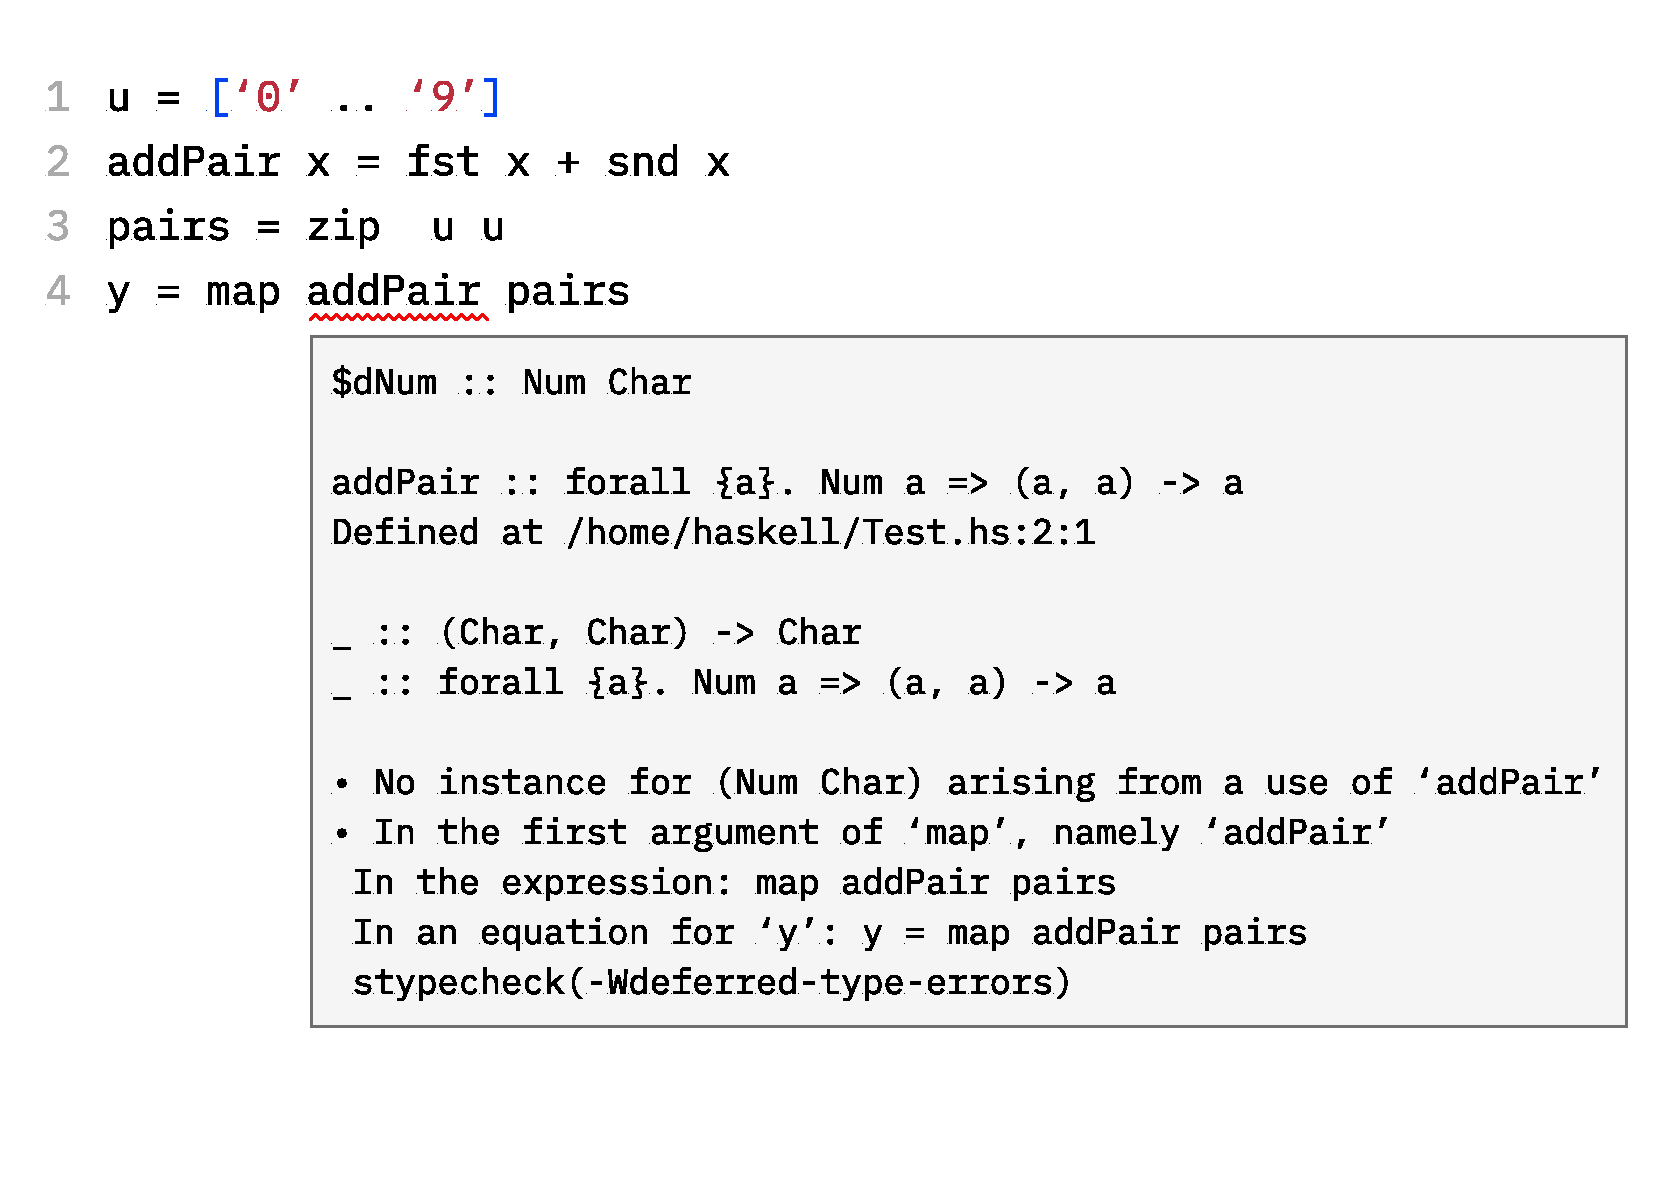
\includegraphics[width=\linewidth,trim=0mm 35mm 0mm 0mm]{Figures/add-pair-example.pdf}
    \caption{
    A type error displayed in Visual Studio Code\cite{microsoft_visual_nodate} and the Haskell Vscode extension~\cite{haskell_haskell_nodate}.
The expression \texttt{addPair} is blamed for causing the type error. This may not match the programmers' intention. 
    }
    \label{fig:motivation-example}
\end{figure}

\subsubsection{\textbf{Traditional type errors show only limited location}}
Haack and Wells~\cite{haack_type_2004} noted that ``\textit{Identifying only one node or subtree of the program as the error location makes it difficult for programmers to understand type errors. To choose the correct place to fix a type error, the programmer must find all the other program points that participate in the error.}'' The type error in Fig.~\ref{fig:motivation-example} can be fixed in multiple locations. For instance  replacing \texttt{['0'..'9']} on line 1 with \texttt{[0..9]}, or replacing \texttt{fst x} and \texttt{snd x} on line 2 with \texttt {read (fst x)} and \texttt{read (snd  x)}. In the type error message, only the \texttt{addPair} expression on line 4 was blamed.  In this small example, the whole context is visible, but it can become problematic in large programs where the lines contributing to the type error are far apart in the source code.

\subsubsection{\textbf{Traditional type errors are biased}}
A common form of bias happens when a type error is reported in one expression, but it can occur in multiple other expressions as well. In Fig.~\ref{fig:motivation-example}, the error message arbitrarily focuses on only \texttt{addPair}, while ignoring that the literals in the definition of \texttt{u} may be incorrect. 

Another form of bias is that traditional type errors are often framed as conflicts between \texttt{Expected type} and \texttt{Actual type}. This framing is standard practice in most typed languages. However, what is \texttt{expected} and what is \texttt{actual} are a side effect of different unification orders rather than the intention of the programmer. In both forms, the error message may lead programmers to falsely believe the validity of parts of code and wrongly accuse others.

\subsubsection{\textbf{Traditional type errors give poor explanations}}
When the compiler rejects a program, the internal state of type checking is the result of a complex computation. But the details of this process are hard to explain to users and are usually not reported by compilers. For the typical type error shown in Fig.~\ref{fig:motivation-example}, the evidence for the type error is gathered from the previous declarations. These have to be rediscovered by programmers using less rigorous methods. 

\subsection{Design Goals of \chameleon{}}
Based on the limitations of traditional type errors, we give the following design requirements for \chameleon{}:

\noindent\textbf{Show} all the possible locations where the type error happened or could have happened.

\noindent\textbf{Explain} type errors avoiding jargon and internal constructs of the type checker.

\noindent\textbf{Do not presume} which expression is to blame for the type error based on the order of computation or which possible type for an expression is `actual' or `expected'.


\section{Features of Chameleon}

Discuss the features of Chameleon, different debugging utilities and modes.

\section{Implementation}

Discuss the implementation of Chameleon. 

\section{Walkthrough}

Explain the interactive features of Chameleon via a semi-realistic debugging example.

\section{Conclusion}

% Chapter 3

\chapter{Effects of Interactive Type Error Debugging Using Chameleon}
\label{chap:chameleon:eval} 

\section{Research Questions}

The studies of Chameleon aim to address the following research question:

\begin{itemize}
	\item Can visual tools help programmers help find bugs?
	\item Can interactive type error narrowing help programmers help solve type errors?
\end{itemize}

\section{Experiment Design}

\subsection{\textbf{Recruitment}}

Participants were recruited via the Reddit \textit{r/haskell} and \textit{r/programminglanguages} communities. 
%Recruiting from social media allowed us to access a more diverse demographic that better represent the true population of Haskell programmers. 
Participation is fully anonymized; detailed ethical implications of these experiments are reviewed and approved by the IRB of the authors' institution.

\subsection{\textbf{Experiment setting}}
Experiments were conducted online and unsupervised. 
%Participants took the study online via a web browser and at the physical venue of their choosing. 
All user studies use a web-based debugging environment developed by the authors. 
%Conducting the studies online helped us avoid variation when performing tasks in unfamiliar places and using different setups. 


\subsection{\textbf{Training and group assignment}}
After consent, participants received interactive training on the tool interface and interactive features. Participants were also shown a cheat sheet summarizing the key functionality of the interface, and had access to the cheat sheet at all times during the study. Participants were given 4 trial runs (2 for each setting) before the data collection started. 
All the studies used a within-subject design to evaluate the effectiveness of different tools or feature sets while counterbalancing the difference in programming proficiency between participants. In each study, participants were required to complete a series of programming tasks (8 for studies 1a and 1b, 9 for study 2). At each task, a participant receives a single Haskell file that contains one or more type errors. They were then asked to correct the code with the help of the given tool.


\subsection{\textbf{Data Collection}}
Time is measured from the start of each task to the first time the program is successfully type-checked and also passes all the functional tests. Participants are able to skip a task if they are stuck. 
% The data is automatically recorded by the online debugging environment. To not introduce a barrier to completing the study, every task can be skipped if the participant made three failed attempts or is stuck for over 1 minute on the task.
After completing all tasks, participants are prompted to complete a debriefing survey. The survey questions include their Haskell experience and feedback on the tools.

We used a browser session recording tool~\cite{openreplay_openreplay_2022} to record the study sessions. This allows us to identify usability issues in the study and to recognize general patterns. 

\section{Results}

\section{Discussion}
\section{Conclusion}
 
% Chapter 4

\chapter{Goanna: Finding All Type Errors Using Minimal Correction Sets} 

\label{chap:goanna} 
\graphicspath{{Figures/Goanna}}

All programming slicing based tools use MUS as underlying data structure to narrow down the potential error locations. MUS is very effective in providing a explanation of why there must be an error. But it also suffer from a few drawbacks. First, the size of MUS can grow very large in certain type of projects, in result, reduced usability. Second, MUS omit crucial information that may play important role in error comprehension. In this chapter, we investigate these drawbacks in detail and describe how we address these drawbacks using another MCS as the underlying data structure for representing type error. We then show how we designed Goanna, an MCS-based type error debugging environment, and how Goanna can better support type error debugging in examples. Lastly, we show how we designed an empirical study to examine the accuracy, conciseness and performance of Goanna.


\section{Introduction} \label{sec:introduction}
    
Statically-typed languages have gained popularity in the mainstream programming world \cite{StackOverflow2022-aw}. Many new languages have been designed with strict type systems, while others have introduced static typing through external tools. Numerous studies indicate that programming with strongly-typed languages can prevent certain errors \cite{Bogner2022-vf}, enhance code quality \cite{Mayer2012-lg}, and reduce maintenance costs \cite{Kleinschmager2012-bg} compared to similarly positioned dynamic languages \cite{Bogner2022-vf}. Despite their increasing popularity and benefits, challenges persist in the real-world adoption of these languages \cite{Zeng2019-ou}. The steep learning curve of complex type systems remains an obstacle to their adoption. 

Haskell is renowned for its expressive and robust type system. It enables programmers to model complex problems as constructs and relations within type systems and develop robust programs in a type-driven style. Historically, many type system innovations initially introduced by Haskell \cite{Hudak2007-kn}, including algebraic data types, type inference, and type classes, have now found their way into mainstream programming languages \cite{TypeScriptTeam_undated-qk,Klabnik_undated-mp,Griesemer_undated-ff}.
    
However, Haskell is also known for its steep learning curve and unforgiving type errors. Numerous research efforts have attempted to address these challenges \cite{Tirronen2015-nr,Chen2014-dz, Heeren2003-kd,Zhang2015-xy, Lerner2007-mu,Zhang2017-tj}. The type errors generated by the most commonly used Haskell compiler, GHC (Glasgow Haskell Compiler), often lead to confusion among novice users, and sometimes experts. For instance, in the program shown in Fig.~\ref{fig:motivation}, a type mismatch between a {\tt Char} type and an integer number type results in a perplexing type error for novice users. We have identified three challenges for making use of these error messages:


    \begin{enumerate}
        \item Fixated on one possible cause while other potential causes exist.
        \item Changing the suggested location does not completely rectify the error.
        \item Not enough contextual information for programmers to understand how the judgment was made.

    \end{enumerate}


    \begin{figure}
        \centering
        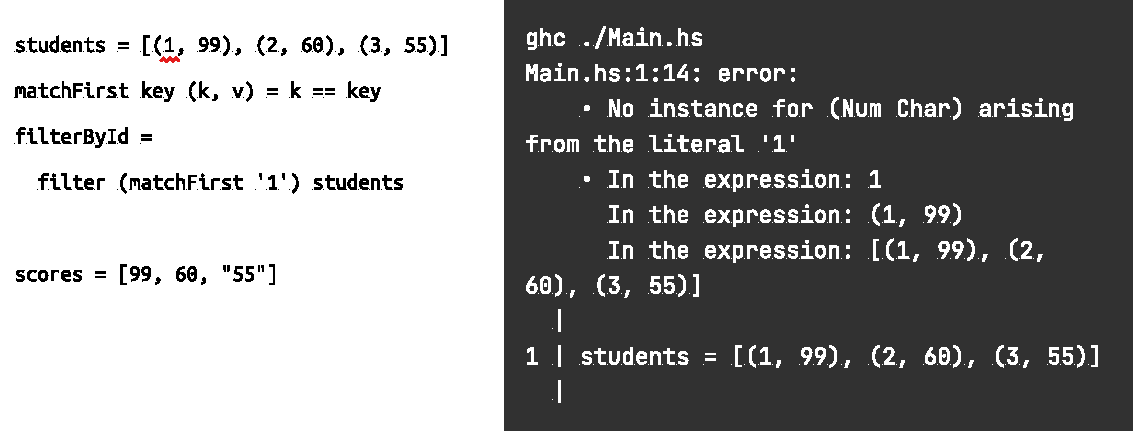
\includegraphics[width=\linewidth]{images/motivation}
        \caption{Inspecting a type error using the Haskell compiler GHC (Glasgow Haskell Compiler)}
        \label{fig:motivation}
    \end{figure}




    To address these challenges of diagnosing and fixing type errors in Haskell, we present a new tool: \textit{Goanna}. Goanna is a Haskell type checker based on Minimal Correct Set (MCS) enumeration. Compared to traditional type-checking tools, Goanna provides improved type error reporting by giving a comprehensive list of possible causes and suggesting valid fixes for each cause.  Goanna differs from past type debugging systems (as reviewed in Section \ref{sec:related-work}) through its use of Minimal Correction Subsets (MCS), where a single MCS represents a complete set of locations that constitutes a possible cause.

	To further enhance Goanna's support for type-error resolution, we provide optimization strategies (Section~\ref{sub:optimization}) to identify and reduce the unhelpful suggestions, as well as ranking heuristics (Section~\ref{sub:ranking}) to suggest more likely fixes first. Additionally, we provide Goanna-IDE, an interactive debugging front-end designed to efficiently navigate and interpret Goanna's type error diagnosis.

    We conducted empirical studies that evaluated Goanna's accuracy (Section \ref{sub:eval-accuracy}), conciseness (Section \ref{sub:eval-conciseness}), and performance (Section \ref{sub:eval-performacne}). Our evaluation shows that compared to other type-checking tools, Goanna consistently provides accurate error diagnostics and correct fixes in its top suggestions. We also demonstrate that Goanna generally offers a concise list of possible causes, thanks to its cause optimization process. While Goanna may not consistently provide instantaneous results for real-time feedback, it can deliver on-demand diagnoses when programmers require additional assistance.
    

    The key contributions of this research include:
    \begin{itemize}
        \item Goanna, a Haskell type checker with improved error reporting based on MCS enumeration and program slicing;
        \item Goanna-IDE, an interactive type error debugging interface for Haskell; 
        \item A collection of heuristics and optimization techniques to enhance MCS-based type error reporting; and
        \item An evaluation of Goanna's accuracy, conciseness, and performance.
    \end{itemize}

  The techniques we used in Goanna, such as MCS enumeration and heuristics for ranking possible causes, are not exclusive to Haskell. Rather, they are applicable to statically typed programming languages in general. We intentionally designed Goanna to use a modular architecture that can be easily extended to support other programming languages with similar typing dicipline.


    \section{Goanna-IDE Walkthrough} \label{walkthrough}
    We first illustrate Goanna's capability by demonstrating the usage of Goanna-IDE. Goanna-IDE is a type error debugging interface for Haskell. It is designed to efficiently navigate and make use of Goanna's type error diagnosis through visualization and interactivity. Goanna-IDE provides comprehensive diagnostic error messages for type errors in Haskell and allows programmers to interactively explore their options. An online demo of Goanna-IDE is available for evaluation at \cite{Anonymous2023-bo}. Goanna-IDE includes a file explorer, a text editor, and a debugging panel. Goanna-IDE provides the following features when type errors are encountered:

    \begin{itemize}
        \item Thoroughly detect all type errors within the codebase and allow users to inspect each type error individually via the debugging panel.
        \item Indicate the most likely causes by star indicators.
        \item Show necessary type hints in the editor panel to help reason about each possible cause.
        \item Allow users to trace type errors across multiple files.
    \end{itemize}

    \subsection{Examples of Diagnosing Type Errors with Goanna-IDE}

    For the type error in the motivating example, Goanna shows 6 possible causes of the error (see top right corner of Fig.~\ref{fig:goanna-example-1}). When focussing on the cause suggested by GHC, instead of highlighting only the literal \texttt{1}, Goanna reports all 3 literals that needed to be changed all at once if the programmer chooses to address this cause. In addition, Goanna also indicates that these integer literals need to be changed to \texttt{Char} type using the inlay type hints on line 1, largely narrowing down the potential ideal fixes. 
    

    \begin{figure}[htb!]
        \centering
        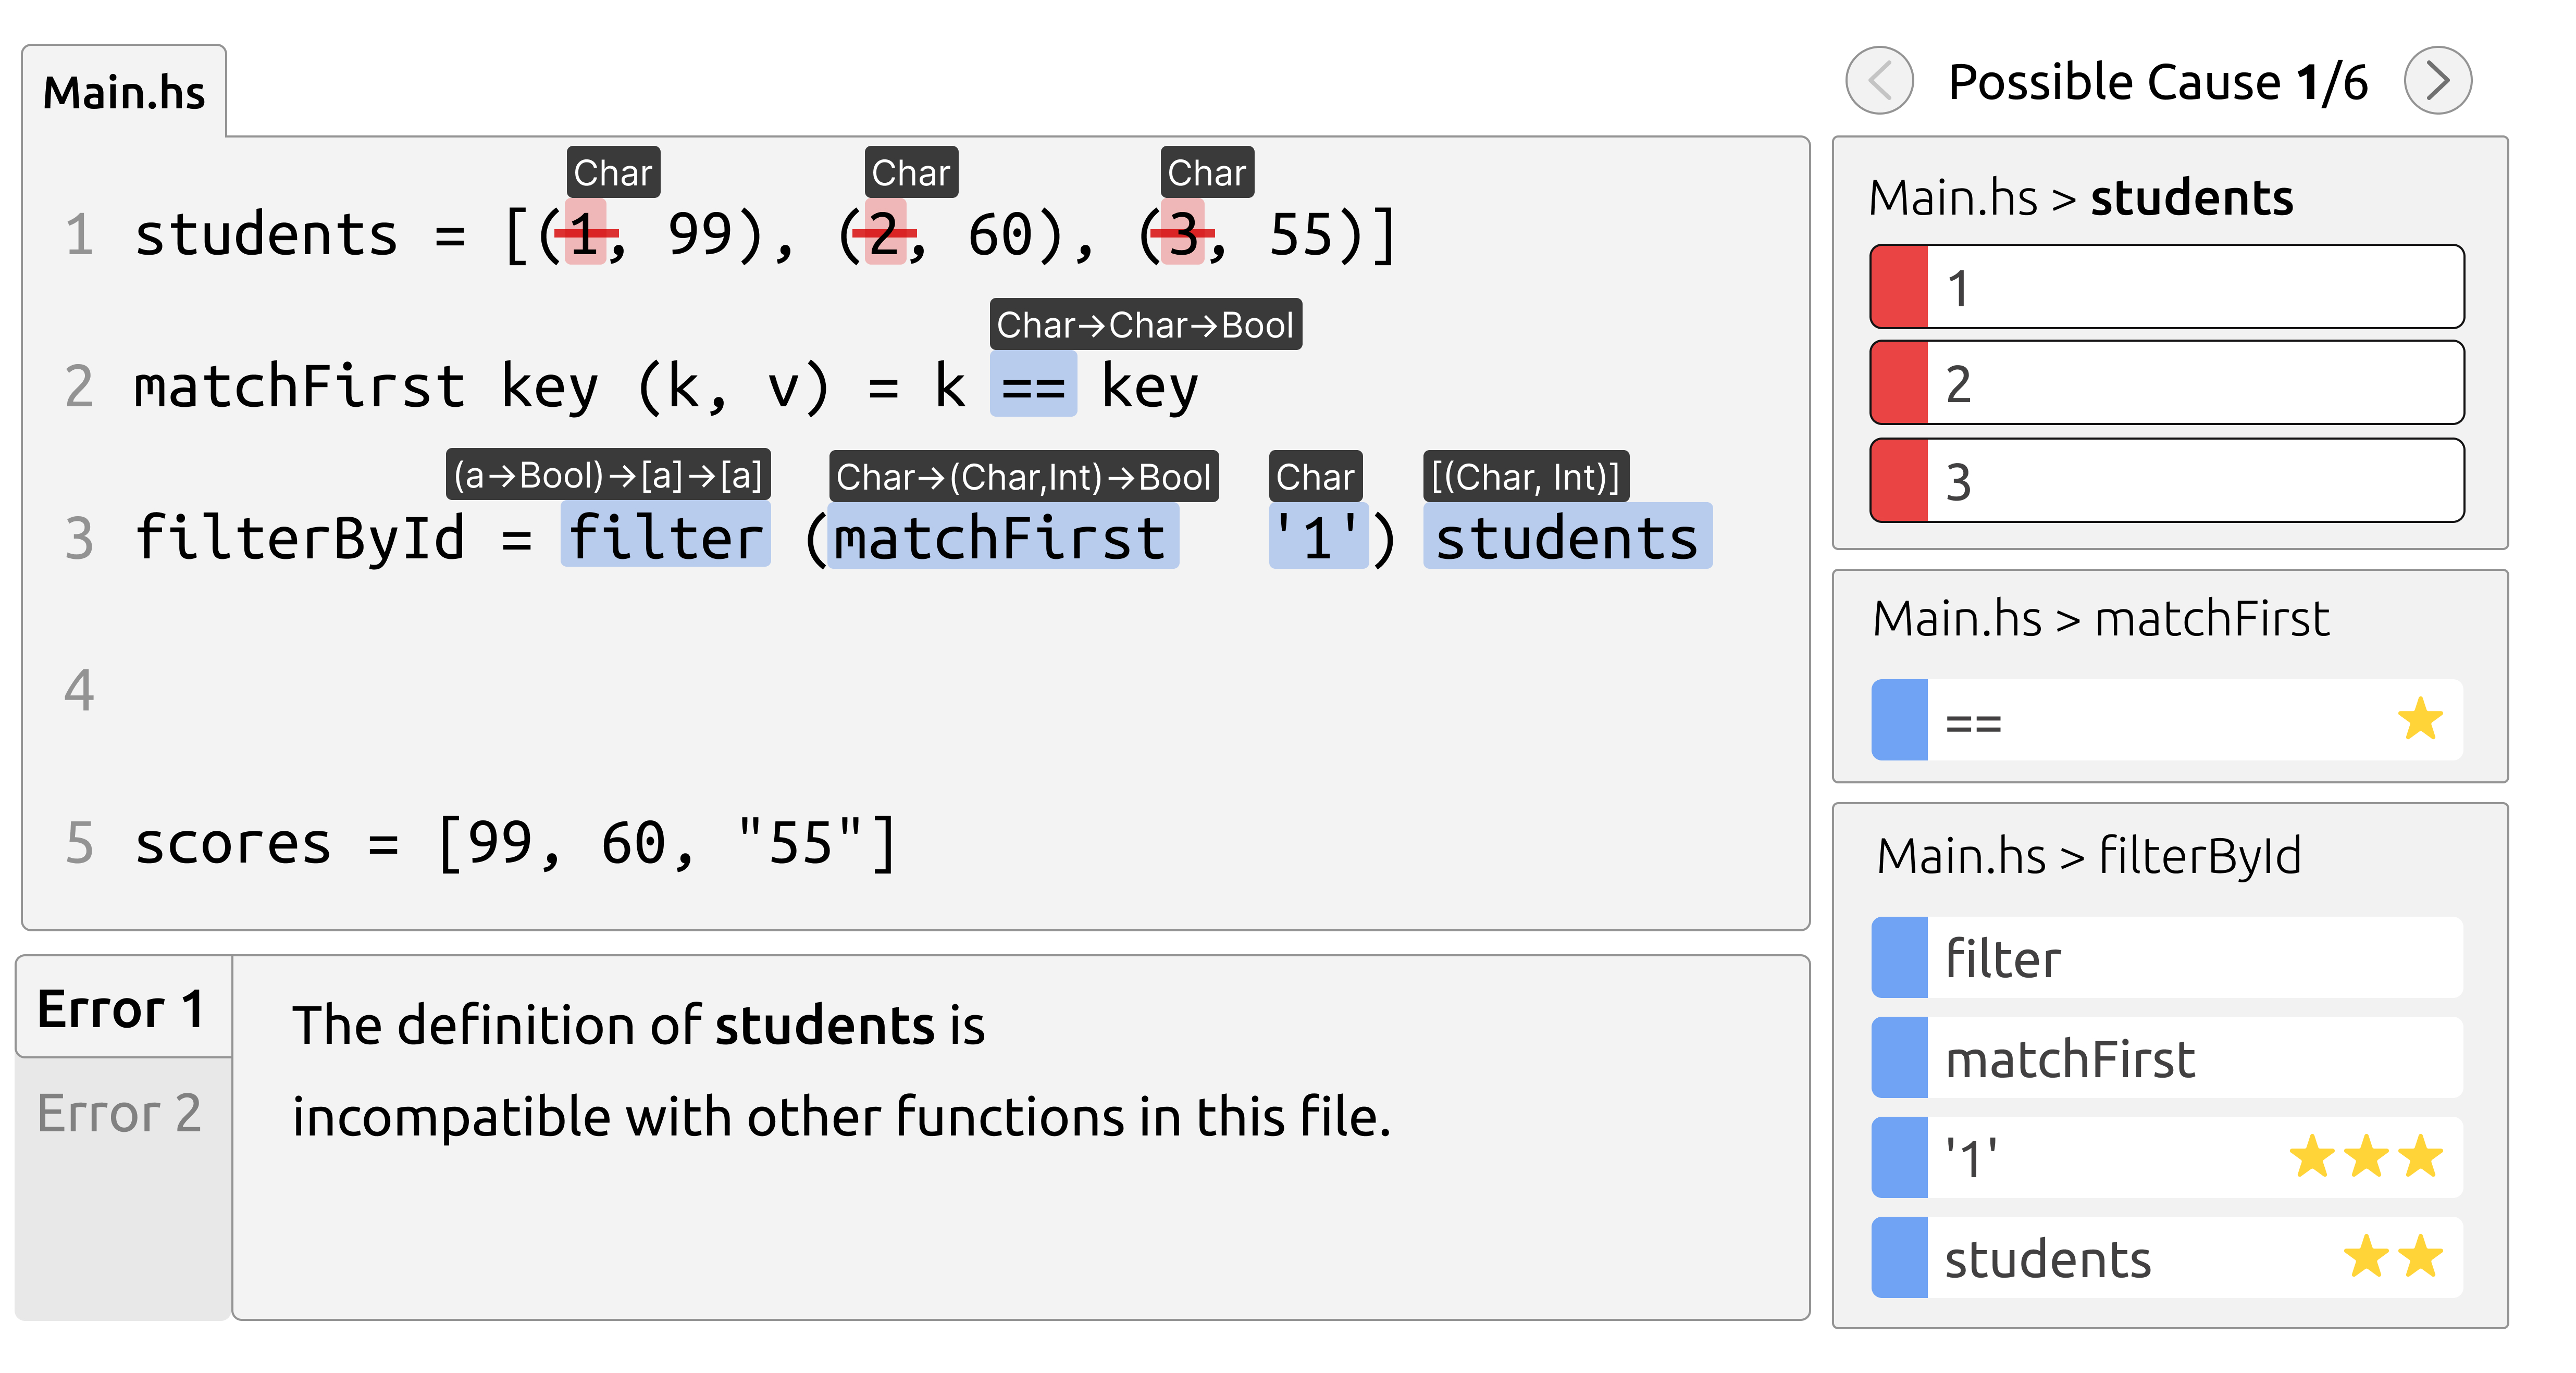
\includegraphics[width=\linewidth]{images/Goanna-Example-1}
        \caption[Goanna's showing possible causes of a type error (1)]{\textbf{Goanna's error diagnosis} Goanna shows that to fix the type error, the literals \texttt{1}, \texttt{2}, and \texttt{3} on line 1 need to be changed to Char type.}
        \label{fig:goanna-example-1}
    \end{figure}


    Note that the cause suggested by GHC is only one of the possibilities identified by Goanna. In fact, Goanna suggests that there are more likely fixes, indicated by the star symbols. The most likely fix, based on Goanna's cause heuristics (Section \ref{sub:ranking}), is the \texttt{Char} literal \texttt{'1'} on line 5, indicated by the 3 stars (Fig.~\ref{fig:goanna-example-1}).
    
    
    By clicking on the most likely cause, Goanna shows different highlights in the editor (e.g. see Fig.~\ref{fig:goanna-example-2}). Goanna reports the error is caused by the literal \texttt{'1'} and suggests changing to an integer. All the type hints are adjusted based on our new assumption. Goanna ranks all possible causes using a series of heuristics. In this case, the preference is largely influenced by how many locations are required to change to fix the error. 
    
    \begin{figure}[htb!]
        \centering
        \includegraphics[width=\linewidth]{images/goanna-example-2}
        \caption[Goanna's showing possible causes of a type error (2)]{\textbf{Goanna's error diagnosis.} Goanna shows that the type error can be fixed by changing the literal $'1'$ on line 3, which needs an \texttt{Int} type. This, according to Goanna, is the most likely cause of the type error.}
        \label{fig:goanna-example-2}
    \end{figure}


    \subsection{Identifying all type errors} \label{sub:all-errors}
    
    A key feature of Goanna is its ability to detect all type errors in the code thanks to its MCS enumeration (Subsection \ref{sub:enumeration}). This is not always the case with other tools, such as GHC, which may only report a subset of the errors present in the code or stop at the first error they encounter. Goanna, however, always thoroughly identifies all type errors in the codebase. In the example of Fig.~\ref{fig:goanna-example-1} and Fig.~\ref{fig:goanna-example-2}, Goanna discovered the two errors included in the file. Clicking on the error selector on the bottom-left will change the content of the debugging panel and text editor highlights to reflect the cause of a different error (Fig.~\ref{fig:multi-error}). 

    \begin{figure}[htb!]
        \centering
        \includegraphics[width=\linewidth]{images/goanna-multi-error}
        \caption[Selecting a different error in Goanna]{\textbf{Selecting a different error in Goanna.} Selecting a different error using Goanna's error selector. The debugging panel will show potential cause locations for the selected error. The highlights and type hints in the editor panel will focus on the selected error.}
        \label{fig:multi-error}
    \end{figure}



    \subsection{Type error grouping}  \label{sub:group}
    In addition to reporting multiple errors, Goanna also groups together type errors that might be treated as separate by other tools. Goanna uses a novel approach (section \ref{sub:grouping}) to ensure that type errors that are intuitively connected are grouped together. This means that Goanna does not overwhelm the programmer with an excessive number of redundant type errors. Instead, the programmer is presented with a concise list of errors that all can be assessed separately.

    \begin{figure}[htb!]
        \centering
        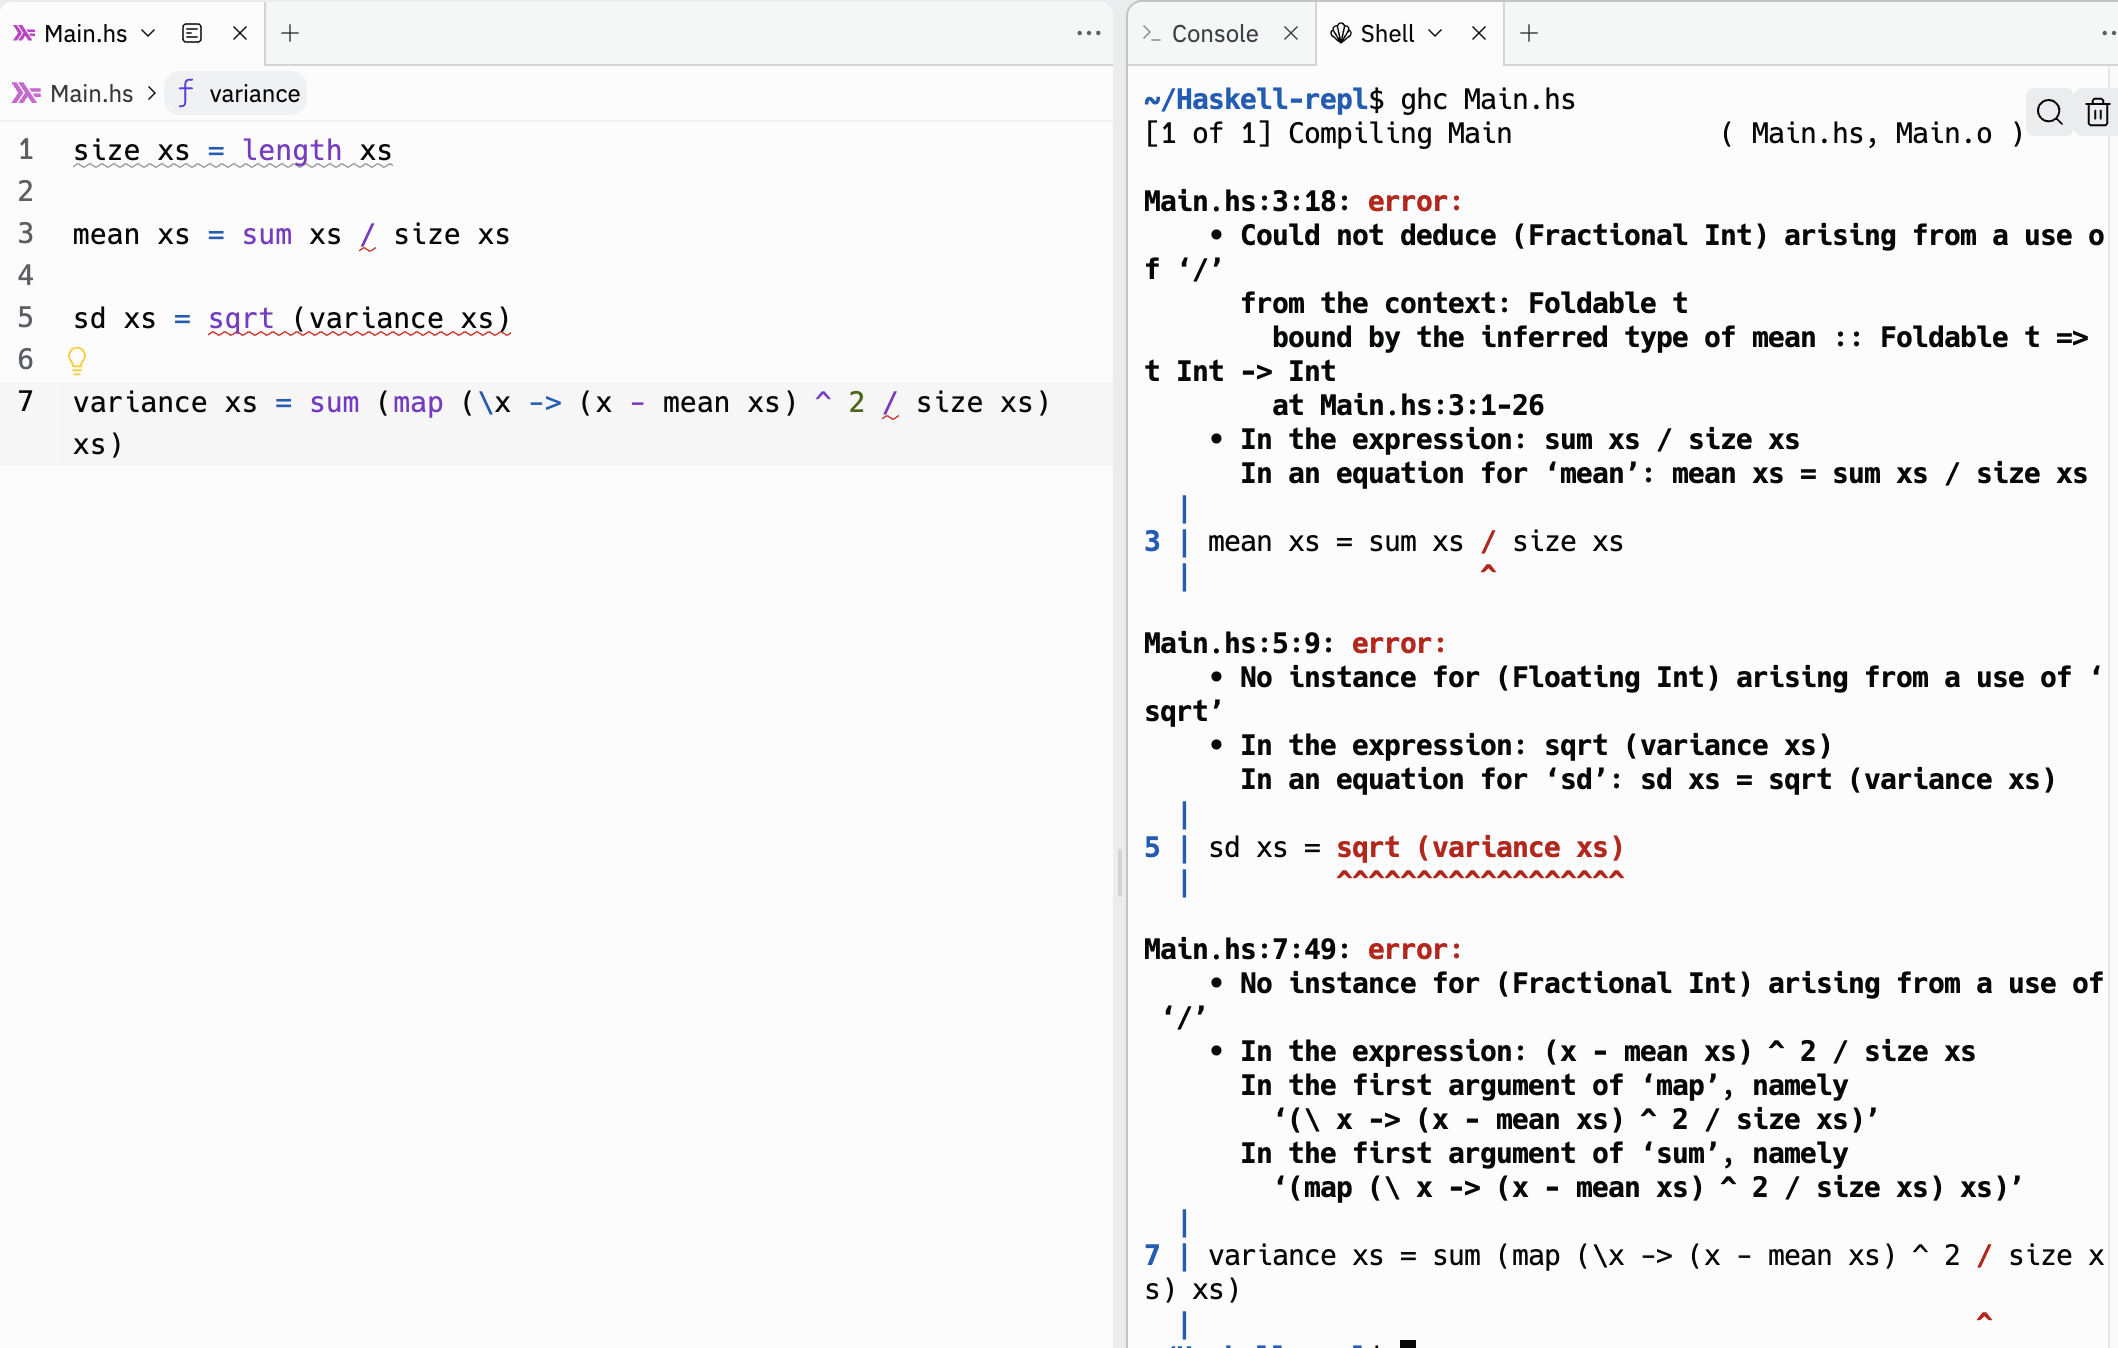
\includegraphics[width=\linewidth]{images/variance-ghc}
        \caption[Inspecting a defective Haskell Program in relation to the error messages output by the standard GHC compiler]{\textbf{Inspecting a defective Haskell Program (left) in relation to the error messages output by the standard GHC compiler (right)} -- 3 separate type errors are reported.  The editor (VS Code is used here) underlines the error locations reported in the messages, but all other contextual information must be understood from the error text.}
        \label{fig:grouping-ghc}
    \end{figure}
    
        \begin{figure}[htb!]
        \centering
        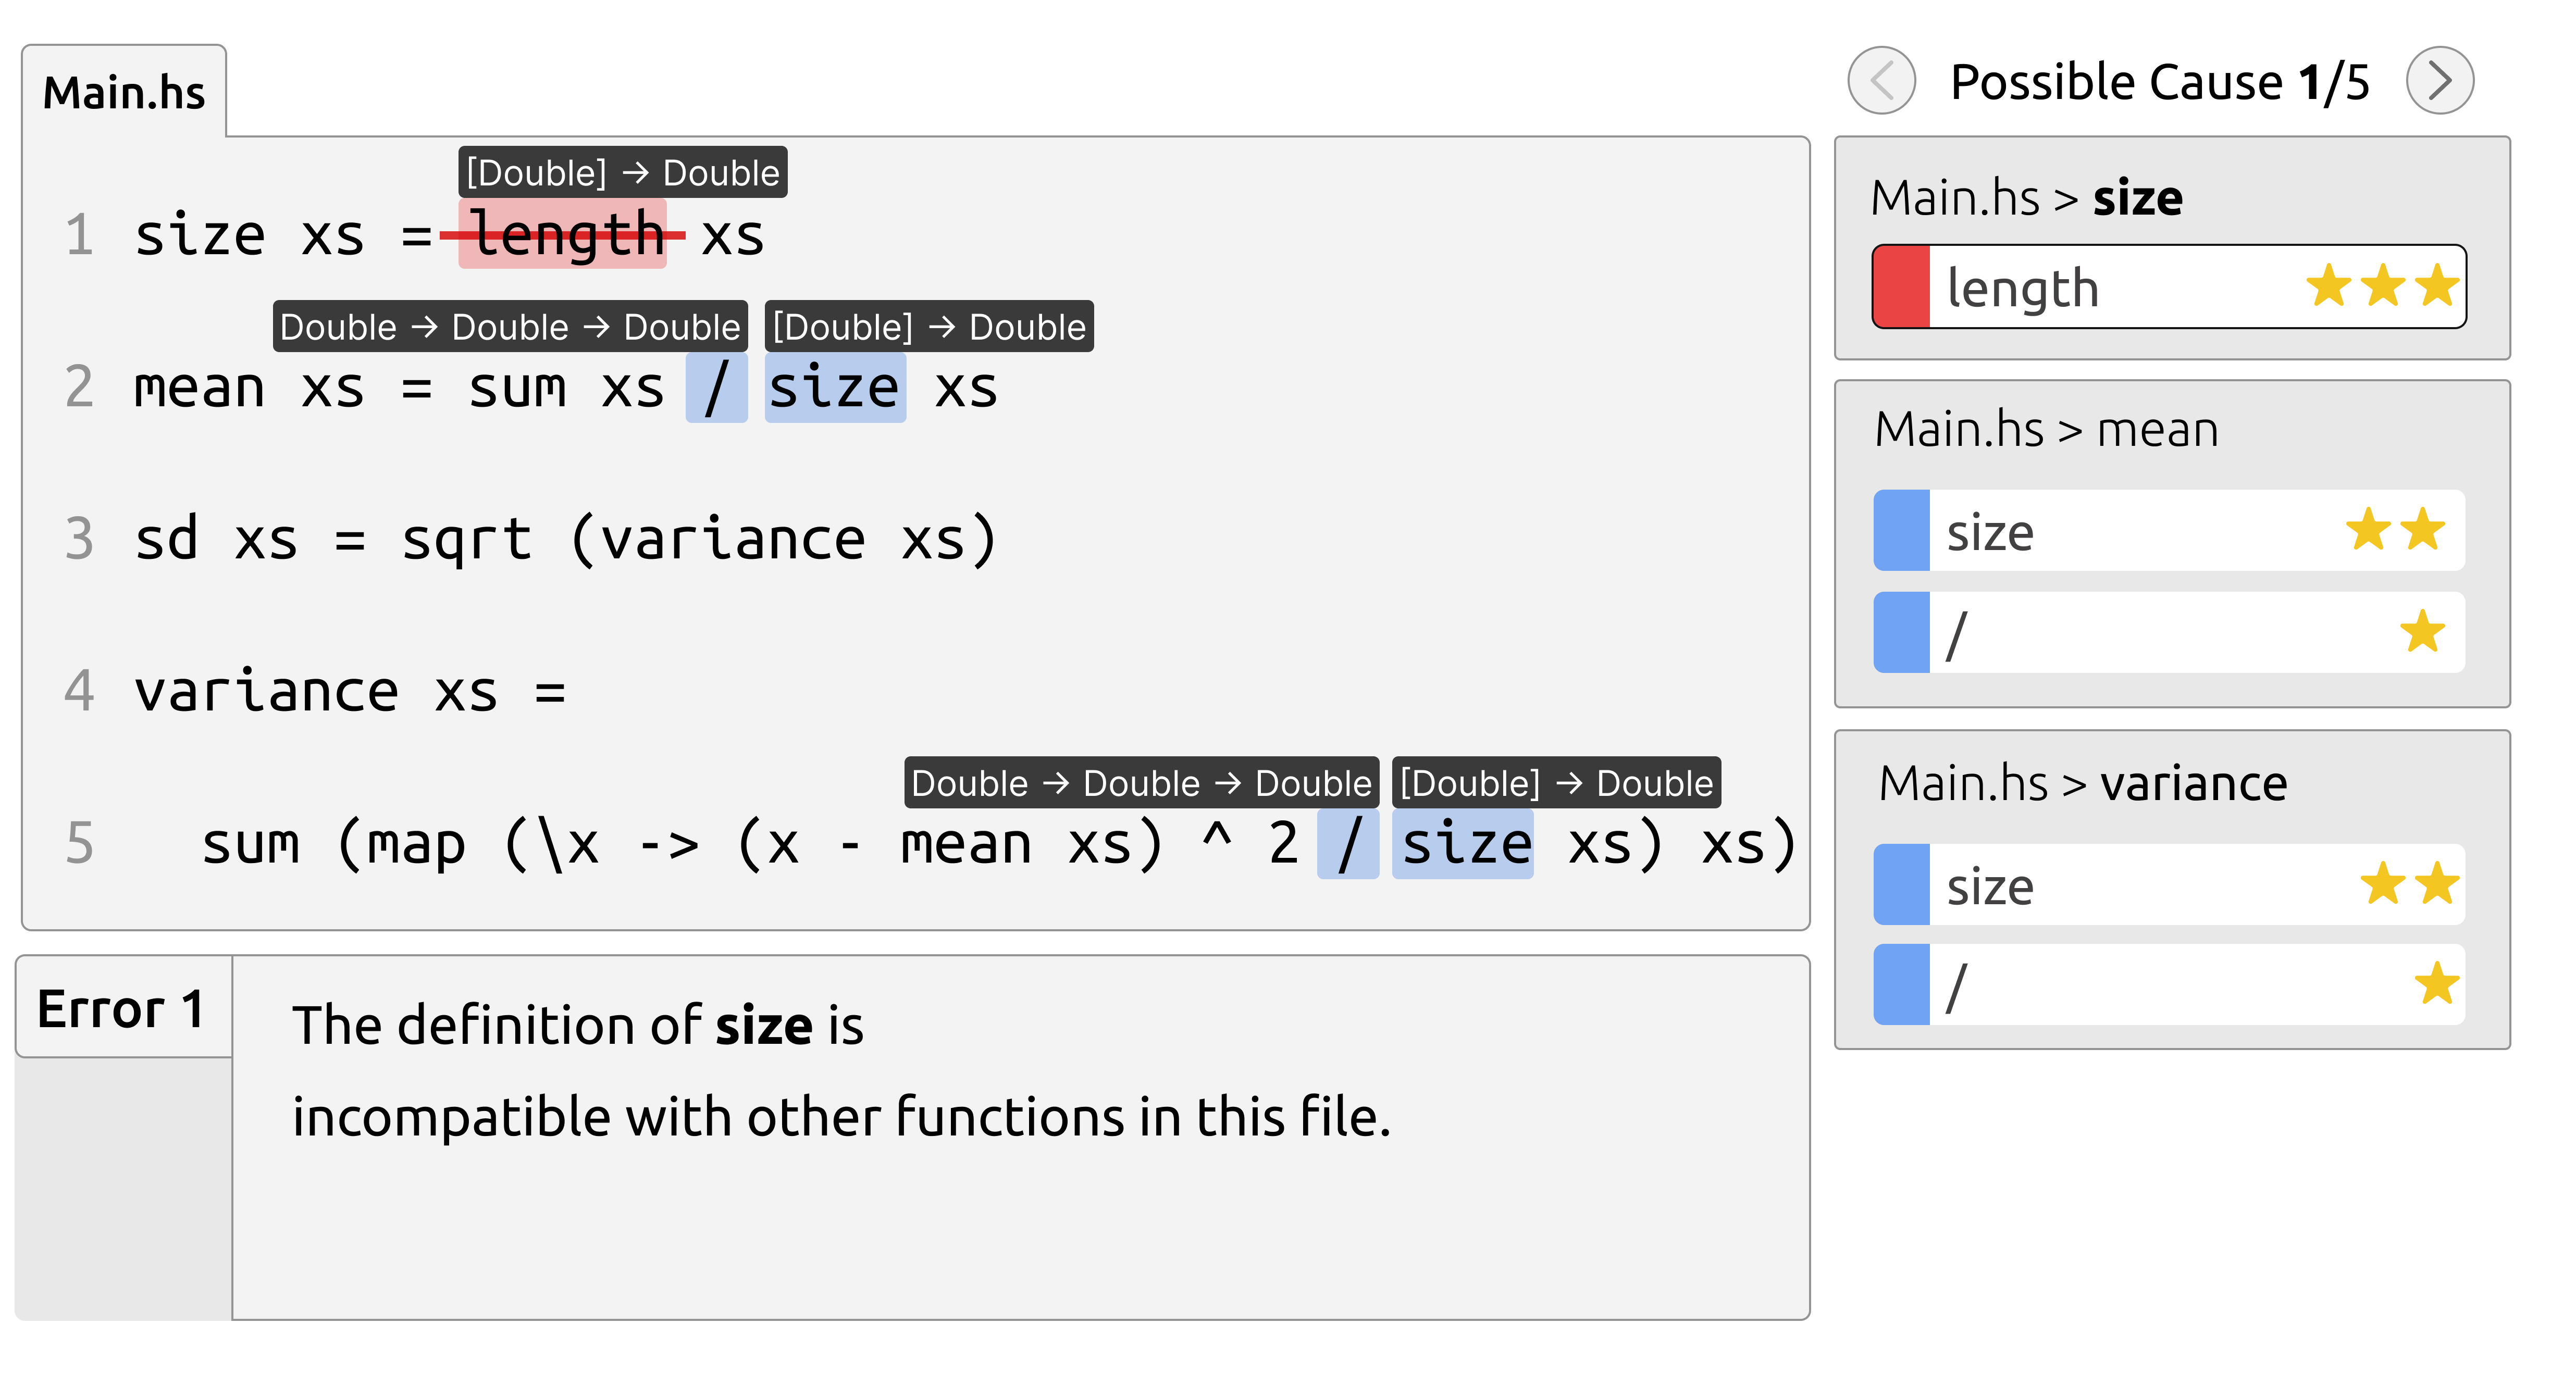
\includegraphics[width=\linewidth]{images/Goanna-Error-Grouping}
        \caption[Goanna's Error Grouping]{\textbf{Goanna's Error Grouping.} This error, although its potential offending parts appear in many declarations, is possible to fix in one place, i.e. by changing the definition of the \texttt{size} function on line 1. Therefore, Goanna reports it as a single error.}
        \label{fig:grouping-goanna}
    \end{figure}

    For instance, in Fig.~\ref{fig:grouping-ghc}, the functions \texttt{variance} and \texttt{mean} expect the final type of \texttt{size} to be a fractional value. However, the definition of \texttt{size} results in an integral value, which creates a conflict. While GHC shows three separate type errors, Goanna groups these interconnected errors into a single entity, as shown in Fig.~\ref{fig:grouping-goanna}. These errors can be addressed collectively, thereby improving the efficiency of the programmer.

    \subsection{Discovering Potential Causes} \label{sub:suggesting}
    When a type error arises, Goanna-IDE shows a list of possible causes in the debugging panel. Each possible cause consists of one or more locations in the code that require modification to rectify the type error. Clicking on a possible cause activates it. The locations are highlighted in the text editor, as well as inlay type hints suggesting the suitable type expected for that code slice. In the debugging panel, the activated cause is outlined with a red icon, while others are marked with a blue icon. 

    The causes identified by Goanna are comprehensive. Goanna will take into account potential causes in expressions, pattern matchings, type annotations, and type class constraints. Consequently, programmers will generally find the real cause by exploring Goanna's diagnosis. Unlike most Hindley-Milner~\cite{Damas1982-sc} based type inference, Goanna does not show a bias towards the unification order, thereby avoiding the left-to-right bias \cite{Chen2014-ev}. 
    
    Note that Goanna's fixes are sufficient for resolving the type error. Traditional tools often reveal a set of partial locations of a type error, leaving programmers to realize later that additional adjustments are needed for a complete resolution. Goanna, however, offers fixes that encompass a complete set of changes necessary for a resolution.


    \subsection{Assessing Likelihood of Causes} \label{sub:conciseness}
    One challenge of Goanna's ``find all causes" approach is the number of ways an error can occur can sometimes become too large to be useful in practice. Goanna employs multiple techniques to intelligently sieve the list. For the remaining list, Goanna employs a few heuristics to rank their likelihood and inform programmers which causes they consider first. 
    Goanna-IDE uses a star-based rating system to signal the ``likelihood'' of each cause. 3 stars indicating the most likely cause, 2 stars and 1 star follows. 

    \subsection{Type Hints}\label{subset:type-hints}
    In addition to suggesting which part causes that type error, Goanna-IDE explains why this is inferred by using in-situ type hints on necessary terms. The type hints are displayed as inlay decorations on top of respective fragments of source code. These type hints provide enough information for programmers to understand the type inference, and Goanna will leave out the terms that are irrelevant to the type error. Goanna's type hints are also dynamic to the selected cause. Programmers can observe how the inferred type of each term changes by changing the selected cause. Many modern programming tools use inlay type hints to support understanding, such as   Haskell Language Server~\cite{HLS-Developers2023-ot},  most often, these tools will display all type hints or none. Unlike in Goanna, these tools do not provide alternative sets of type hints for programmers to compare.
    
    \subsection{Cross-module type error debugging}\label{subsec:cross-module-type-error-debugging}
    When encountering a type error spanning across multiple modules, Goanna-IDE will group the potential causes indicated by their module and declaration block. Clicking on any possible cause location will focus the editor on the corresponding module (Fig.~\ref{fig:goanna-cross-module}). Goanna is the first tool to introduce cross-module type debugging. The way Goanna presents cross-module type errors is analogous to how run-time errors are presented in most programming languages. When encountering a run-time error, most programming environments show a call stack containing multiple file paths, and programmers can choose which file to start investigating. Often, programmers choose to start from the file authored by themselves instead of library files. Goanna uses this mental model to group potential locations that cause a type error by module and definition blocks. 
    
    \begin{figure}[htb!]
        \centering
        \includegraphics[width=\linewidth]{images/goanna-cross-module}
        \caption[Debugging a cross-module error in Goanna]{\textbf{Debugging a cross-module error in Goanna.} In this error, potential defects may appear in either module \texttt{A} and \texttt{B}. Goanna suggests 3 potential causes and fixes: 1) Change the type annotation of \texttt{x} to \texttt{[Maybe Int]} (Top). 2) Change the y variable on line 4 of module \texttt{A} to an instance of \texttt{Int}. 3) Change both the elements in the list literal in module \texttt{B} (Bottom), hence affecting the type of \texttt{y}. Clicking on each potential cause in the debugging panel results in different highlights and type hints in the editor panel.}
        \label{fig:goanna-cross-module}
    \end{figure}



    \section{Goanna Implementation} \label{sec:implementation}
    Goanna comprises 3 phases: constraint generation, MCS enumeration, and post-analysis. In the constraint generation phase, Goanna walks the abstract syntax tree and collects constraints. In the MCS enumeration phase, Goanna enumerates through all MCSes. Lastly, in the post-analysis phase, Goanna applies multiple optimization techniques to reduce the number of MCSes, group MCSes by common properties, and sort them based on heuristics.

    \subsection{Haskell Coverage}
    Goanna supports a wide and growing range of the Haskell 2010 language syntax \cite{Simon_Marlow2010-lg}. At the time of writing, fully supported features include module import/export, qualified imports, import hiding, do notation, algebraic data type, new type, type synonym, type class, operator sectioning, range expression, N+K pattern, with record syntax and list comprehension are under development. Goanna does not yet support type features enabled through language extensions. However, they are also on the roadmap. A detailed and updated feature coverage list can be found in \cite{Anonymous2023-rp}.

    \subsection{Constraint Generation} \label{sub:translation}
    Goanna uses the abstract syntax tree of the original Haskell program and translates it into a constraint program by modeling how types are defined and used. Goanna does not restrict which constraint language and solver should be used. The only requirement is that Goanna needs to be able to assert whether a subset of the constraints is still feasible by calling a provided \texttt{solve} function during the MCS enumeration phase. In our implementation, we generate portable Prolog predicates \cite{Wielemaker2011-sr}. The \texttt{solve} function executes a predefined predicate \texttt{type\_check/0} that tests all the generated predicates. We used standard Prolog notation \texttt{name/arity} here when referring to Prolog predicates, as a Prolog predicate is identified by the combination of both attribute. 

    
    For a simplified Haskell syntax shown in Fig.~\ref{fig:translation}.A, we generate a list of Prolog predicates in the language shown in Fig.~\ref{fig:translation}.B. We use 3 auxiliary functions during the constraint translation process (Fig.~\ref{fig:translation}.C) to generate Prolog variables for future unification. \texttt{fresh} makes a unique unbound Prolog variable. \texttt{var} takes a Haskell identifier name and returns a Prolog variable. Naively, this can be done by turning it to uppercase. \texttt{atom} takes a Haskell type constant/constructor name and returns a Prolog atom. Naively, this can be achieved by turning it into lowercase. We keep track of local variable names in a list $\Gamma$ containing Haskell variable names. A global variable $\mathcal{P}$ is defined to store the list of predicates being generated. To clarify two , all \textcolor{blue}{parsed Haskell syntax} are in blue. All \textcolor{red}{generated Prolog syntax} are in red. 
    
    Two sets of generation rules apply to different syntax nodes and output Prolog source code. Predicate generation rules (Fig.~\ref{fig:translation}.D) take Haskell declarations as input and output Prolog predicates. For example, a Haskell function \texttt{f = 2}, Goanna may generate a predicate \texttt{\textcolor{red}{f(V, \_) <- V = int.}}
    
    Constraints generation rules (Fig.~\ref{fig:translation}.E) take a Haskell expression node or type node and a Prolog variable \texttt{V} as input and output a list of Prolog terms. These terms attempt to unify the inferred type of such node to the provided Prolog variable \texttt{V}.
    
    \begin{figure}[htb!]
        \centering
        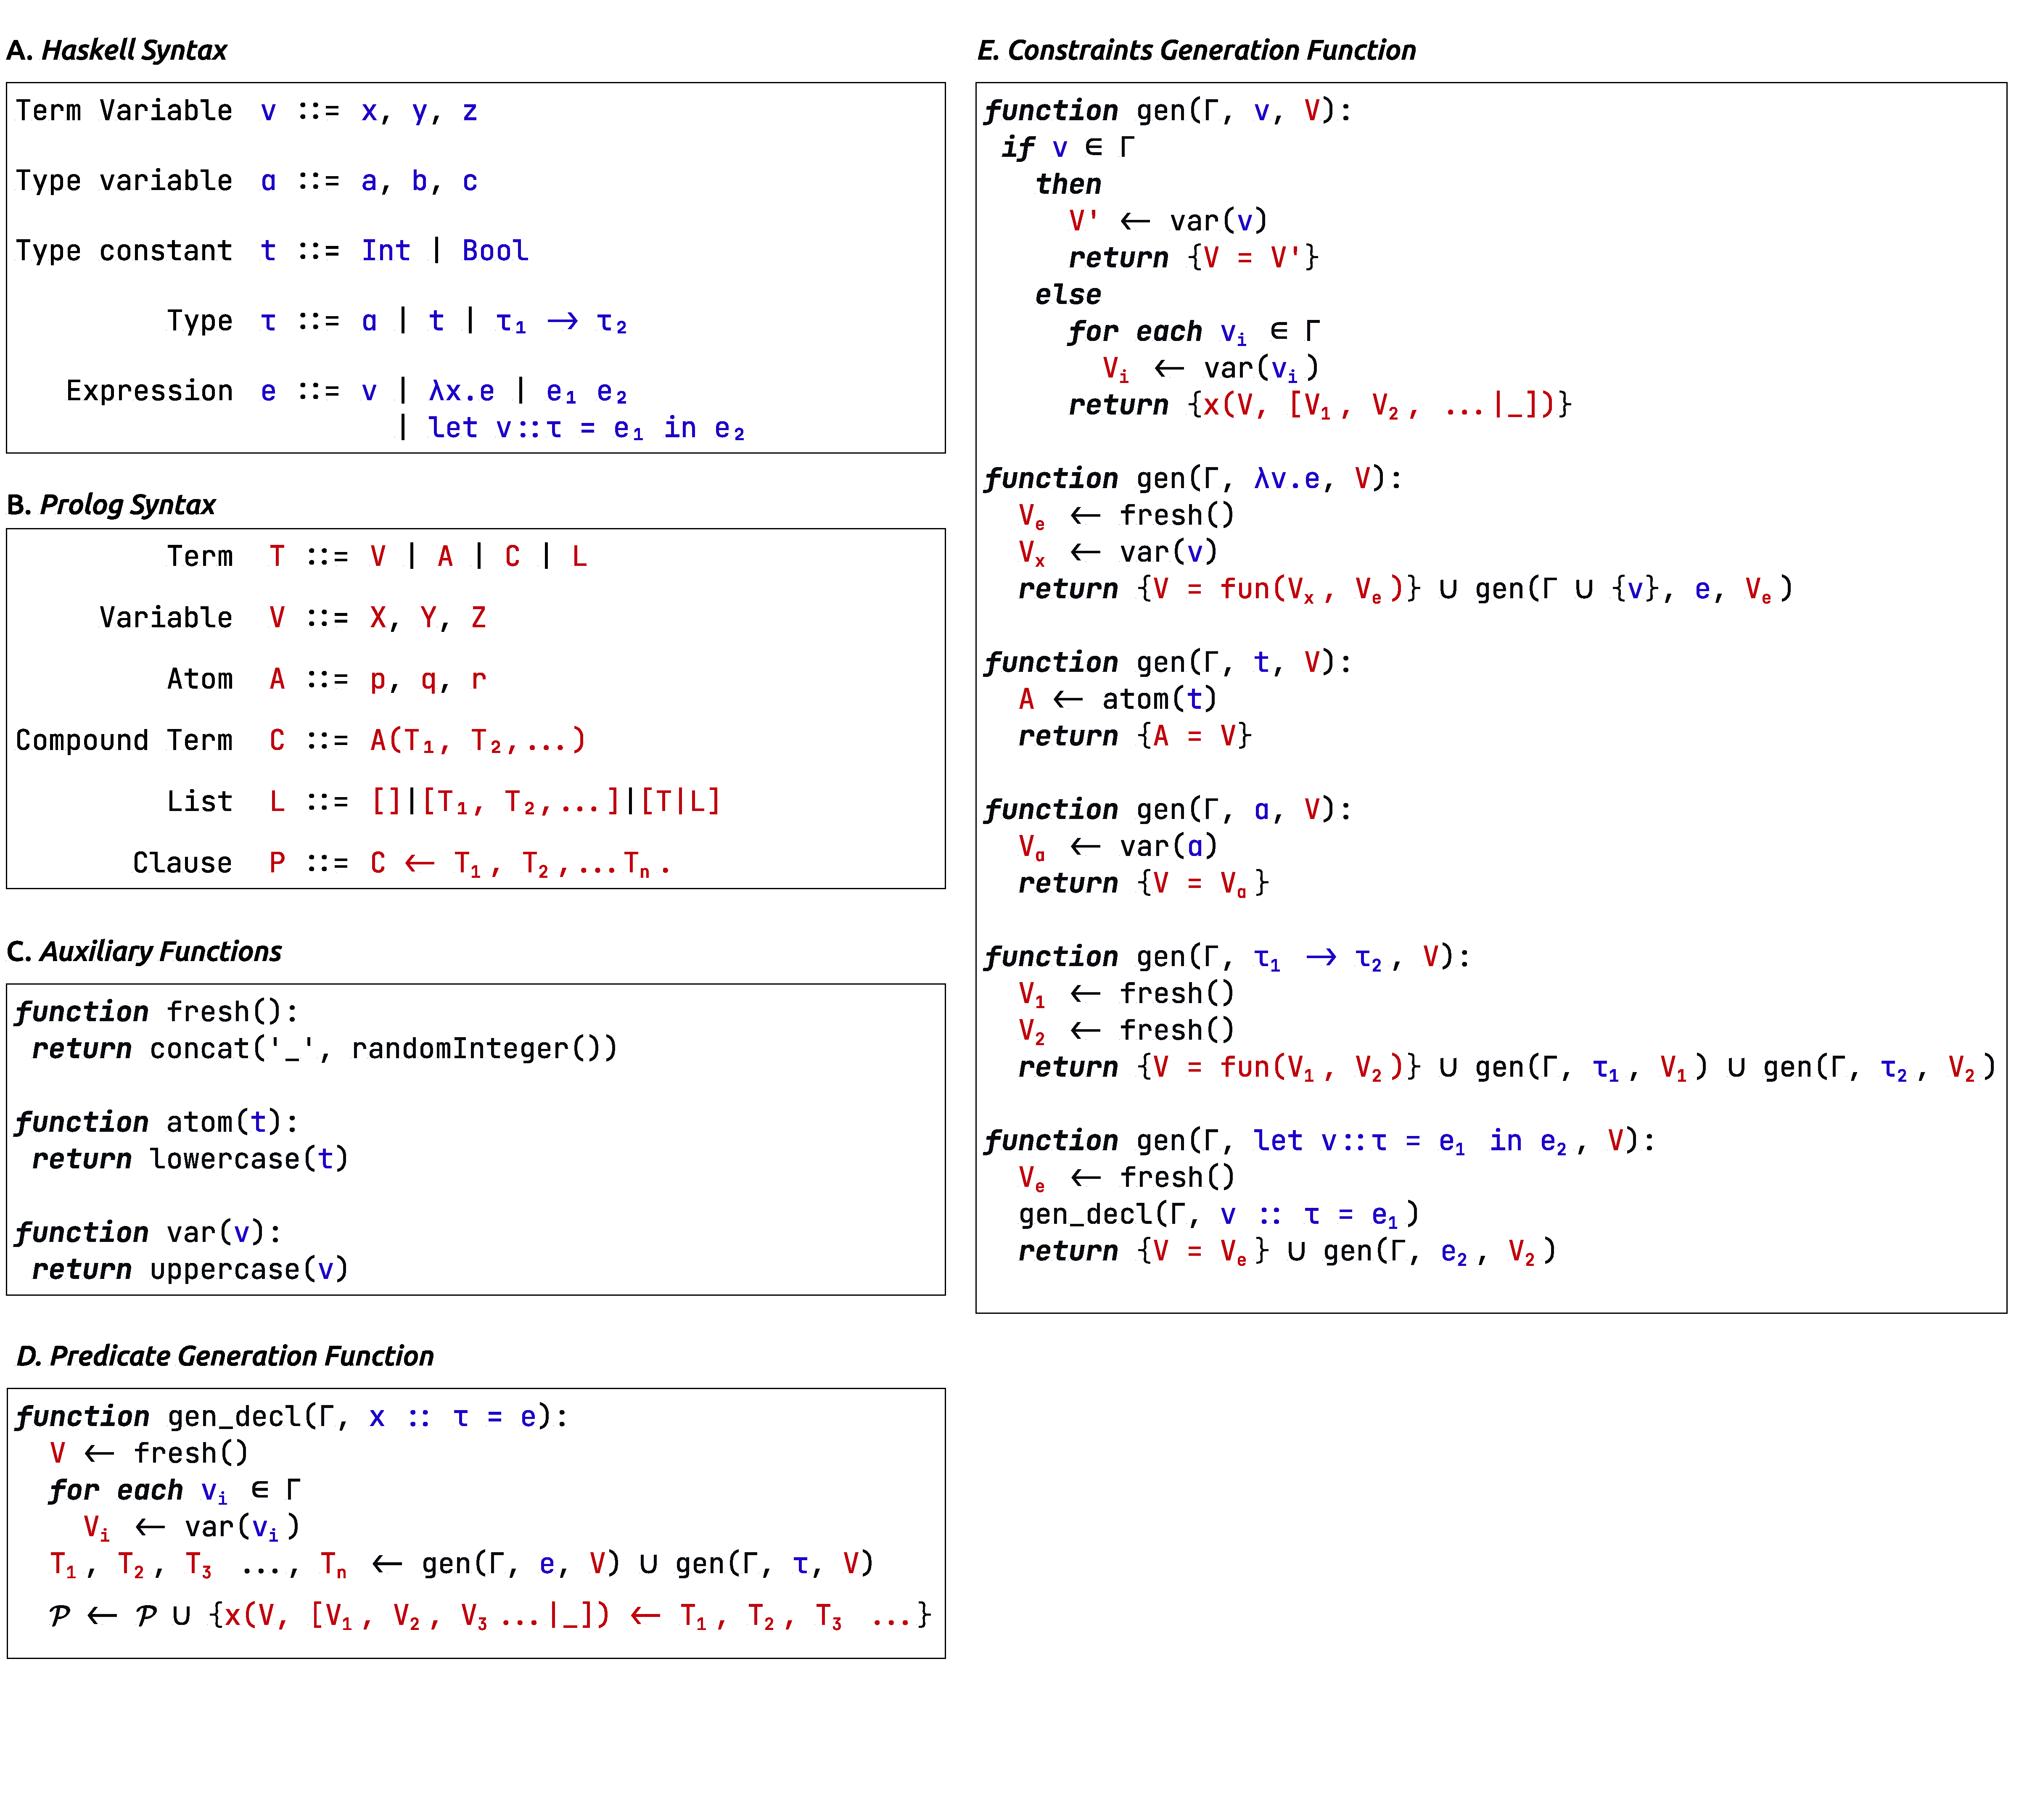
\includegraphics[width=\linewidth]{images/Generation}
        \caption{Goanna's Constraint Translation Rules (Simplified)} 
        \label{fig:translation}
    \end{figure}
    


    \begin{figure}[htb!]
        \centering
        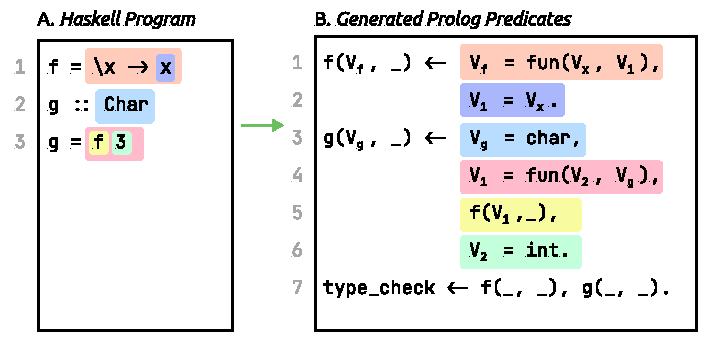
\includegraphics[width=0.8\linewidth]{images/Translation-Example}
        \caption[An example of Goanna constraint generation]{\textbf{An example of Goanna constraint generation.} For the Haskell functions \texttt{f} and \texttt{g}, Goanna generates the predicates \texttt{f/2} and \texttt{g/2}. Each subgoal of \texttt{f/2} and \texttt{g/2} is generated from a corresponding part of the Haskell program. In a predefined predicate \texttt{type\_check/0}, the subgoals \texttt{f(\_,\_)} and \texttt{g(\_,\_)} are added. Running the goal \texttt{type\_check} will return whether the program is well-typed. In this particular example, this will return \texttt{false}. We used standard Prolog notation \texttt{name/arity} here when referring to Prolog predicates, as a Prolog predicate is identified by the combination of both attribute. 
}
        \label{fig:translation-example}
    \end{figure}
    

    An example of such translation can be found in Fig.~\ref{fig:translation-example}. In the Haskell program (Fig.~\ref{fig:translation-example}.A), 2 functions are declared: \texttt{f} and \texttt{g}. This will generate two corresponding Prolog predicates \texttt{f/2} and \texttt{g/2}. In the actual implementation of Goanna, the generated predicates would be \texttt{f/6} and \texttt{g/6}. The extra arguments are added to perform various tasks involving syncing state, such as breaking recursive calls, and collecting type class constraints. In a predefined predicate \texttt{type\_check/0}, the subgoals \texttt{f(\_,\_)} and \texttt{g(\_,\_)} are added. Executing the top-level goal \texttt{type\_check} in a Prolog environment will get a result of \texttt{false}.

    \subsection{MCS enumeration} \label{sub:enumeration}
    After the constraint generation phase, Goanna obtains a list of constraints derived from the source code and is able to query the feasibility of any subset of the constraint system by calling the \texttt{solve} function. Using a known algorithm \cite{Liffiton2016-xi}, Goanna then derives some useful subsets of the constraint system through MCS enumeration. We refer to the complete set of constraints as a constraint system $C$. When we use the word subset without specifying the corresponding superset, it can be inferred as the subset of the constraint system $C$. We list these subsets obtained from MCS enumeration and give their type-theoretic interpretation. 
    
        
    – A minimal unsatisfiable subset (MUS) $M$ of a constraint system $C$ is a subset $M \subseteq C$ such that $M$ is unsatisfiable and $ \forall{c} \in M : M \setminus \{c\}$ is satisfiable. An MUS can be seen as a minimal explanation of the constraint system’s infeasibility. MUSes have been used extensively, mostly in combination with programming slicing, as a means to explain type errors. A MUS of type system constraints reasoning chain connecting all evidence from one location of the conflict to another. Goanna uses the set of all MUSes to group related type errors.

    – A minimal correction set (MCS) $M$ of a constraint system $C$ is a subset $M \subseteq C$ such that $C \setminus M$ is satisfiable and $\forall{S} \subset M : C \setminus S$ is unsatisfiable. MCSes are so named due to the fact that their removal from $C$ can be seen to “correct” the infeasibility. In an ill-typed program, an MCS $C$ can be seen as the ``cause" of a type error; the removal of C will result in the system being well-typed. Goanna uses MCS to represent potential causes of a type error. Each MCS contains the set of locations needed to change to fully resolve the type error.
    
  – A maximal satisfiable subset (MSS) $M$ of a constraint system $C$ is a subset $M \subseteq C$ such that M is satisfiable and $\forall{c}\ in\ C \setminus M:M\cup\{c\}$ is unsatisfiable. The definition of an MSS is symmetric to that of a MUS, with “satisfiable” and “unsatisfiable” swapped along with maximal for minimal. MCS and MSS are the complement sets of one another. In an ill-typed program, an MSS $M$ can be seen as the resulting typing environment if a type error is fixed by excluding the MCS $C - M$. Goanna uses an MSS to provide type hints for the program even when it is ill-typed.
  
%  MCS enumeration has been previously studied for its application in error detection and fault identifications \cite{bekkouche_exploration_2015,lamraoui_formula-based_2016}. And the techniques of MCS enumeration have been improved through many studies \cite{liffiton_fast_2016,zhao_parallelizing_2016,bendik_must_2020}. Unlike previous tools \cite{stuckey_interactive_2003,haack_type_2004}, which use a single MUS, Goanna is the first to use MCS enumeration -- deriving all MUSes, MSSes, and MCSes -- in type error detection and localization. Goanna uses an implementation of the MARCO \cite{Liffiton2016-xi} algorithm to enumerate all MCSes.

 
     \begin{figure}[htb!]
        \centering
        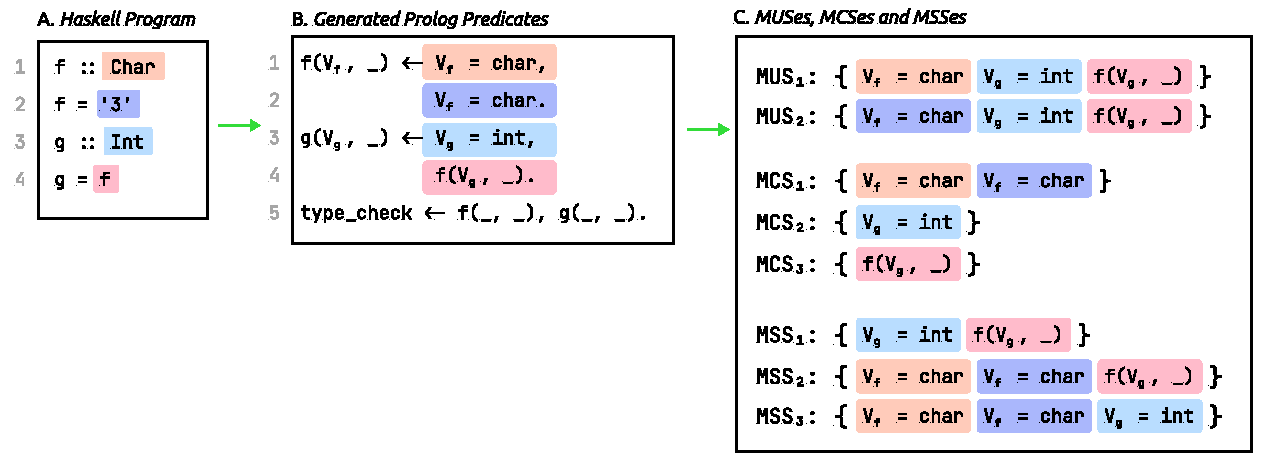
\includegraphics[width=\linewidth]{images/Enumeration-Example}
        \caption[An example of Goanna MCS Enumeration]{\textbf{An example of Goanna MCS Enumeration.} From the set of constraints (B) generated from the Haskell program(A), Goanna obtained 2 MUSes, 3 MCSes, and 3 MSSes. }
        \label{fig:enumeration-example}
    \end{figure}
    
   For the example in Fig.~\ref{fig:enumeration-example}, Goanna's MCS enumeration system identifies 2 MUSes, 3 MCSes, and 3 MSSes. Following the 3 MCSes, Goanna reports 3 potential causes of the type error: the type annotation and function definition in \texttt{f} (from $MCS_1$), the type annotation alone in \texttt{g} (from $MCS_2$), and the function definition alone in \texttt{g} (from $MCS_3$). 
   
   %    \[
%        \begin{array}{c}
%            MUSes = \{\{4, 8\}, \{6, 8\}, \{8, 10\} \} \\
%            MCSes = \{\{8\}, \{4, 6, 10\}\}            \\
%            MSSes = \{\{1,2,3,4,5,6,7,9,10,11,12\},\{1,2,3,5,7,8,9,11,12\}\}
%        \end{array}
%    \]
%
%
%    In the example shown in Fig. \ref{fig:translation}, Goanna suggests two possible fixes: Fix 1 is represented by the MCS ${8}$, and the resulting types are inferred from the MSS ${1,2,3,4,5,6,7,9,10,11,12}$. Fix 2 is represented by the MCS ${4, 6, 10}$, and the resulting type is inferred from the MSS ${1,2,3,5,7,8,9,11,12}$.

%    \subsection{Improvement over MUS-based type error slicing} \label{sub:vs-slicing}
%    In conventional program slicing approaches, a Minimal Unsatisfiable Subset (MUS) is typically used to represent a single type error, thereby providing locations for the type error report. However, we have identified two significant limitations inherent in MUS-based localization and diagnosis:
%
%    \paragraph{Type error localization based on a single MUS only present partial evidence}
%    The minimality of MUS necessitates its exclusion of constraints leading to the same unification. Consequently, MUS-based tools often overlook certain evidence in the code that appears redundant. Programmers, however, are typically interested in obtaining an intuitive understanding of a program defect, not merely a concise proof. For instance, in the program illustrated in the listing \ref{listing:functionf}, MUS-based type error reporting would identify the conflict between the Char literal pattern and one of the three Integer patterns. However, it overlooks the crucial fact that three instances are suggesting \texttt{f:: Num a => String -> a}, while only one suggests \texttt{f::Num a => Char -> a}. With the knowledge of all MUSes, Goanna understands that the constraint that restricts the argument to be of \texttt{Char} type is present in all three MUSes. This allows Goanna to address the discrepancy of evidence in its fix suggestions.
%    \begin{lstlisting}[language=Haskell, caption={An erroneous function definition},captionpos=b, label={listing:functionf} ]
%f "A" = 1
%f "B" = 2
%f 'C' = 3
%f "D" = 4
%    \end{lstlisting}
%
%    \paragraph{Limited Reduction Capability of Single MUS-Based Type Error Localization}
%    MUS-based error slicing can effectively eliminate program locations that are not contributing to a type error. However, research indicates that program slicing can effectively reduce only around 30\% of the code size that is required to understand a type error \cite{binkley_empirical_2007}. Further reduction is challenging with the knowledge of MUS alone due to the MUS's minimality. For instance, in the code shown in listing \ref{listing:functionf}, regardless of the constraint system, if a final MUS is obtained, it must contain at least two constraints that unify the term of the function named \texttt{f} to its respective definition head. This information, "the multiple definition heads must define a function of the same type," rarely contributes to a deeper understanding of type error. It could unnecessarily divert programmers' attention if it holds the same priority as other, more convincing evidence. Compared to MUSes, Goanna uses MCSes, which break down all possible locations into smaller sets and have great flexibility to prioritize and deprioritize location sets.


% \begin{figure}
%     \centering
%     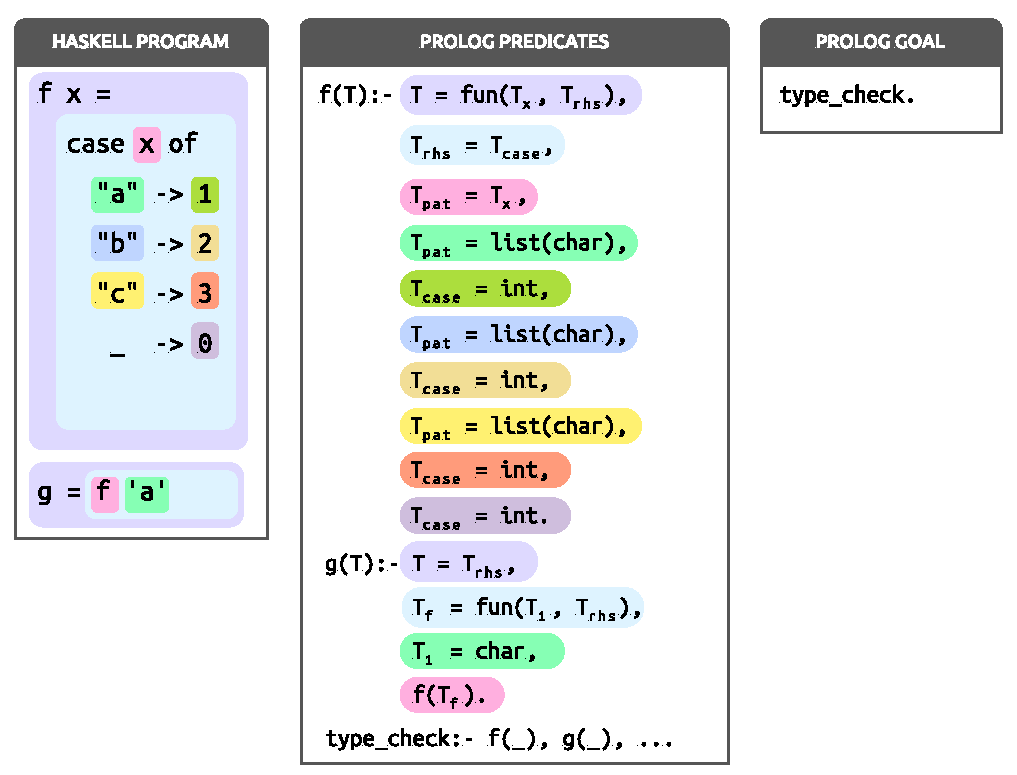
\includegraphics[width=\linewidth]{assets/Translation.pdf}
%     \caption{An example of Goanna generating type constraints.}
%     \label{fig:translation}
% \end{figure}

	\subsection{Post-Analysis}
	Three types of post-analyses are performed by Goanna to improve the quality of error diagnoses: type error grouping, cause ranking, and cause reduction. 
    \subsubsection{Type Error Grouping} \label{sub:grouping}

    Type error grouping is a novel feature provided by Goanna. Conventionally, in a type error slicing approach, a type error is represented by a minimal unsatisfiable subset (MUS). With multiple MUSes available, we have the knowledge to be more precise about an ill-typed program. We propose a novel method of representing type errors that aligns more closely with their colloquial meaning.

	Let $U$ denote the set of all Minimal Unsatisfiable Subsets (MUSes) and $C$ the set of all Minimal Correction Sets (MCSes). We define an undirected graph $G$, where each vertex in $G$ corresponds to a minimal unsatisfiable subset $u_i \in U$, and the edges of $G$ connect pairs of MUSes $u_i$ and $u_j \in U$ if their intersection is non-empty. The set of all connected components $D$ in $G$ represents the set of all type errors. For each $d_i \in D$, let $l_i = \bigcup v_i$, where $v_i$ is the set of vertices in $d_i$. $l_i$ is the set of all constraints local to this type error. Define $C_i = \{ x \mid \forall c \in C, x = c \cap l_i \}$ as the set of all MCSes that are local to this type error.


    This can be intuitively thought of as follows: two type errors can be grouped together if they cannot be fixed independently through modifying a minimal set of locations for each. For instance, Fig.~\ref{fig:grouping-example}.A shows one connected type error, where there are two fixes available: change \texttt{0} on line 1 to a Boolean type, change the type annotation on line 3 to a \texttt{Num} instance, or change the assignment of \texttt{y} to a different expression. Choosing either one will result in both \texttt{x} and \texttt{y} being inferred to have a valid type.
    
    

   \begin{figure}[htb!]
        \centering
        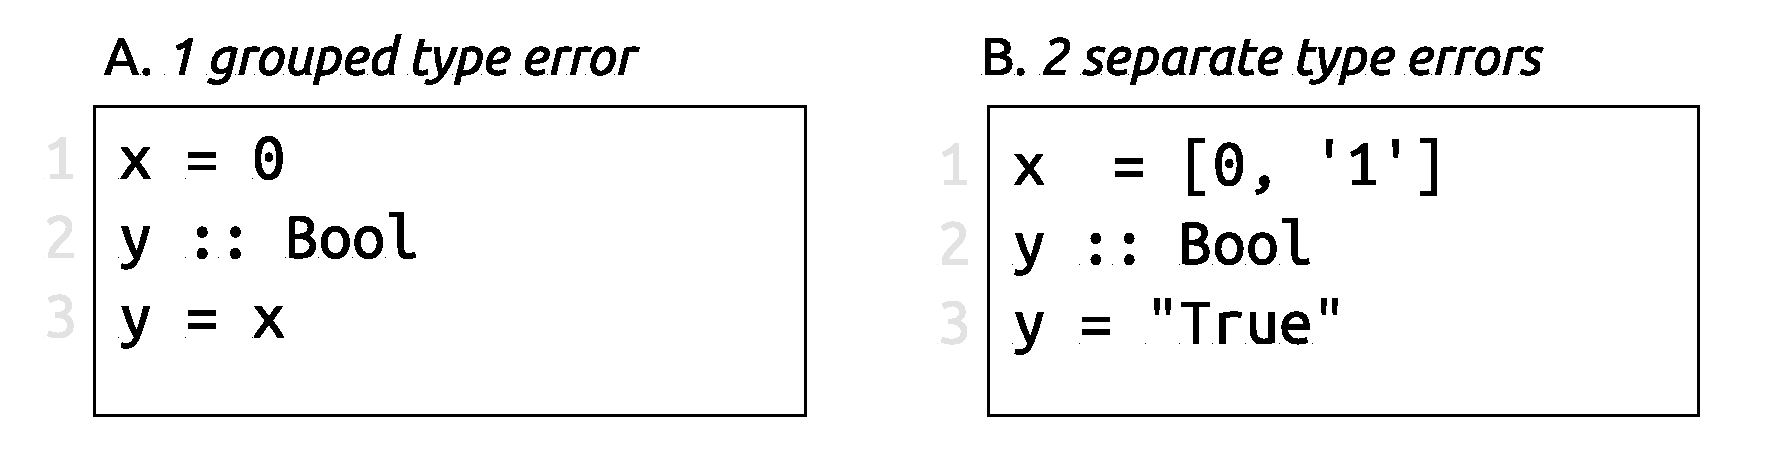
\includegraphics[width=0.8\linewidth]{images/Grouping-Example}
        \caption[Goanna's type error grouping]{\textbf{Goanna's type error grouping.} The ill-typed program on the left contains a single type error, because it can be fixed by a minimal set of syntax changes. For example, fixing it by changing the literal \texttt{0} on line 1 to \texttt{True} or \texttt{False}. This edit contains a single location, so there exists no smaller edit that can fix \texttt{x} or \texttt{y} alone. The program on the right contains two type errors because \texttt{x} or \texttt{y} can be fixed separately. For example change \texttt{0} to \texttt{'0'} on line 1 fix \texttt{x} alone. }
        \label{fig:grouping-example}
    \end{figure}



    However, in Fig.~\ref{fig:grouping-example}.B, although the ill-typed fragment is in a single function, we can fix the argument, either \texttt{0} to \texttt{'0'} or \texttt{'1'} to \texttt{1} to eliminate part of the type error. The same goes for the function's result type \texttt{x}. In this case, there are two separate type errors that should not be grouped.

	
	In practice, type error grouping provides a sense of the ``effective area" of a type error. Programmers are commonly bewildered by the fact that changing one place of the program causes an error in a seemingly unrelated area. When refactoring a known correct program, a programmer can change the definition of one variable, and Goanna will show all the locations that require further changes. This works because all the further changes belong to the same type error group, because a single syntax change -- reverting the initial change -- will result in the program being well-typed once more.
	
	More specifically, to Goanna, type error grouping provides an effective means to reduce the number of causes. In an ill-typed program with $m$ errors, each having $n$ potential causes, will result in $nm$ total causes. Dividing these causes into separate errors that align correctly with intuition is the most important technique to enhance Goanna's error reporting.

    \subsubsection{Cause Ranking} \label{sub:ranking}
     In Goanna-IDE, when a list of potential causes is on display, Goanna-IDE also shows the top 3 ``likely" causes according to the ranking heuristics. This is very helpful because programmers will have a starting point for the investigation. We have identified several efficient heuristics for ranking suggestions. Although no single heuristic ensures universal applicability,  a healthy combination of all the listed heuristics delivers satisfactory results across a broad spectrum of error scenarios.

    \paragraph{Number of Error Locations.}
    Causes comprising fewer locations are prioritized and presented earlier in the list. For instance:
   \begin{figure}[htb!]
        \centering
        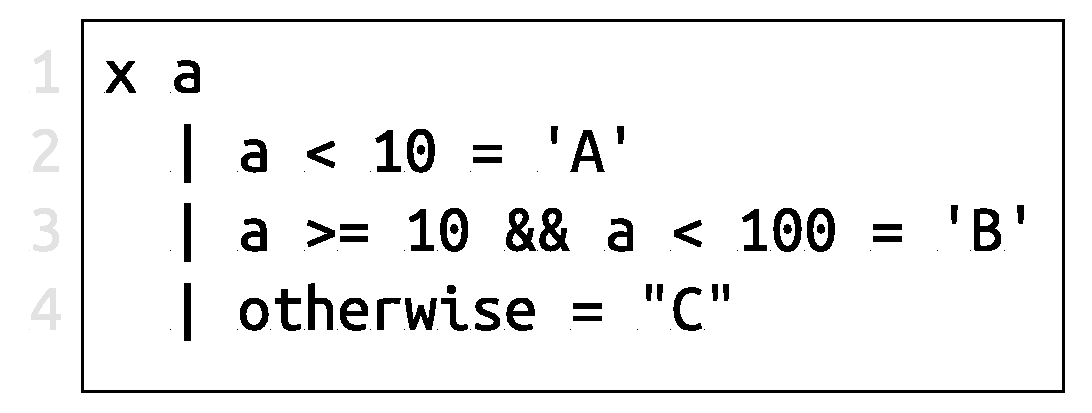
\includegraphics[width=0.5\linewidth]{images/Loc-Count}
        \caption[Goanna prefers causes with fewer error locations]{\textbf{Goanna prefers causes with fewer error locations.} In this ill-typed program, Goanna chooses to give the cause \texttt{"C"} on line 4 a higher likelihood because it contains a single location. The other cause contains 2. }
        \label{fig:loc-count}
    \end{figure}

    In the example in Fig.~\ref{fig:loc-count}, there exist two possible fixes: 1) Changing \texttt{'A'} and \texttt{'B'} to the string type, and 2) changing \texttt{"C"} to the \texttt{Char} type. As the latter fix affects only 1 location (as opposed to 2 in the former), it is assigned a higher ranking and appears earlier in the list.

    \paragraph{Change specificity.}
	Another useful heuristic is to encourage the cause whose fix will result in every surrounding term to be as concrete as possible.
	
	
   \begin{figure}[htb!]
        \centering
        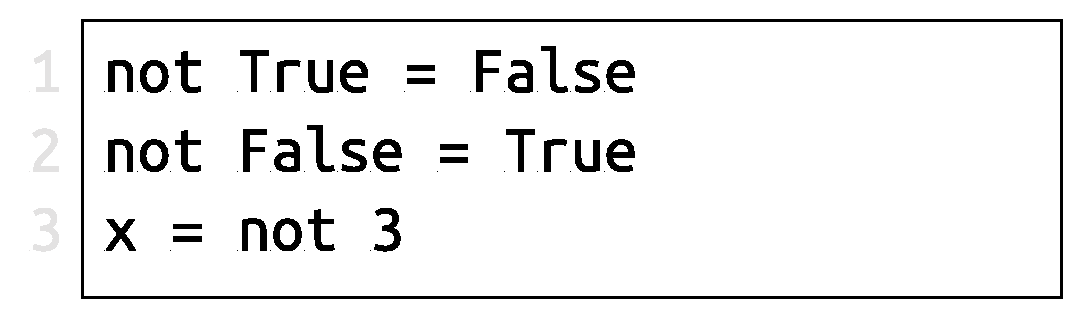
\includegraphics[width=0.5\linewidth]{images/Specificity}
        \caption[Goanna prioritize causes whose resolutions lead to more concrete type assignments]{\textbf{Goanna prioritize causes whose resolutions lead to more concrete type assignments.} In this example, change \texttt{3} will result in \texttt{x} to have type \texttt{Bool}. Alternatively, \texttt{x}'s type will be unknown after changing \texttt{not} on line 3. Goanna prefers the former.} 
        \label{fig:specificity}
    \end{figure}

    In the example in Fig.~\ref{fig:specificity}, Goanna can suggest two potential causes and fixes. First, change the integer literal \texttt{3} to a \texttt{Bool} type. Second, change the function \texttt{not} to a different function that accepts an integer as input. The second fix results in variable \texttt{x} having a less concrete type. Indeed, \texttt{x} can have any type if not limit what function to replace \texttt{not} with. Goanna prioritizes the first cause over the second. 

    \paragraph{Error span.}
    Goanna prioritizes the potential causes whose corresponding locations are clustered within fewer function definitions and lowers the likelihood of those whose corresponding locations being spread across multiple definitions or even multiple files.  

    
    \subsubsection{Cause reduction} \label{sub:optimization}
    
    We employ three techniques to elevate the clarity of the suggestion list: reduction of constraint count, elimination of over-fitting resolutions, and elimination of redundant fixes.

    \paragraph{Minimize Constraint Count.}
    The number of constraints directly influences the time complexity associated with enumerating the Minimum Correction Subset (MCS). By merging multiple constraints into a singular one, we can reduce the total count of constraints and, in turn, improve the performance of enumeration. Yet, this approach requires careful application, as it could potentially lead to unsolvable situations or propose infeasible fixes, as the combined locations in the source code must either all contribute to the type error or none do. An effective application of this technique is to merge all constraints created by sub-expressions in a type signature.

   \begin{figure}[htb!]
        \centering
        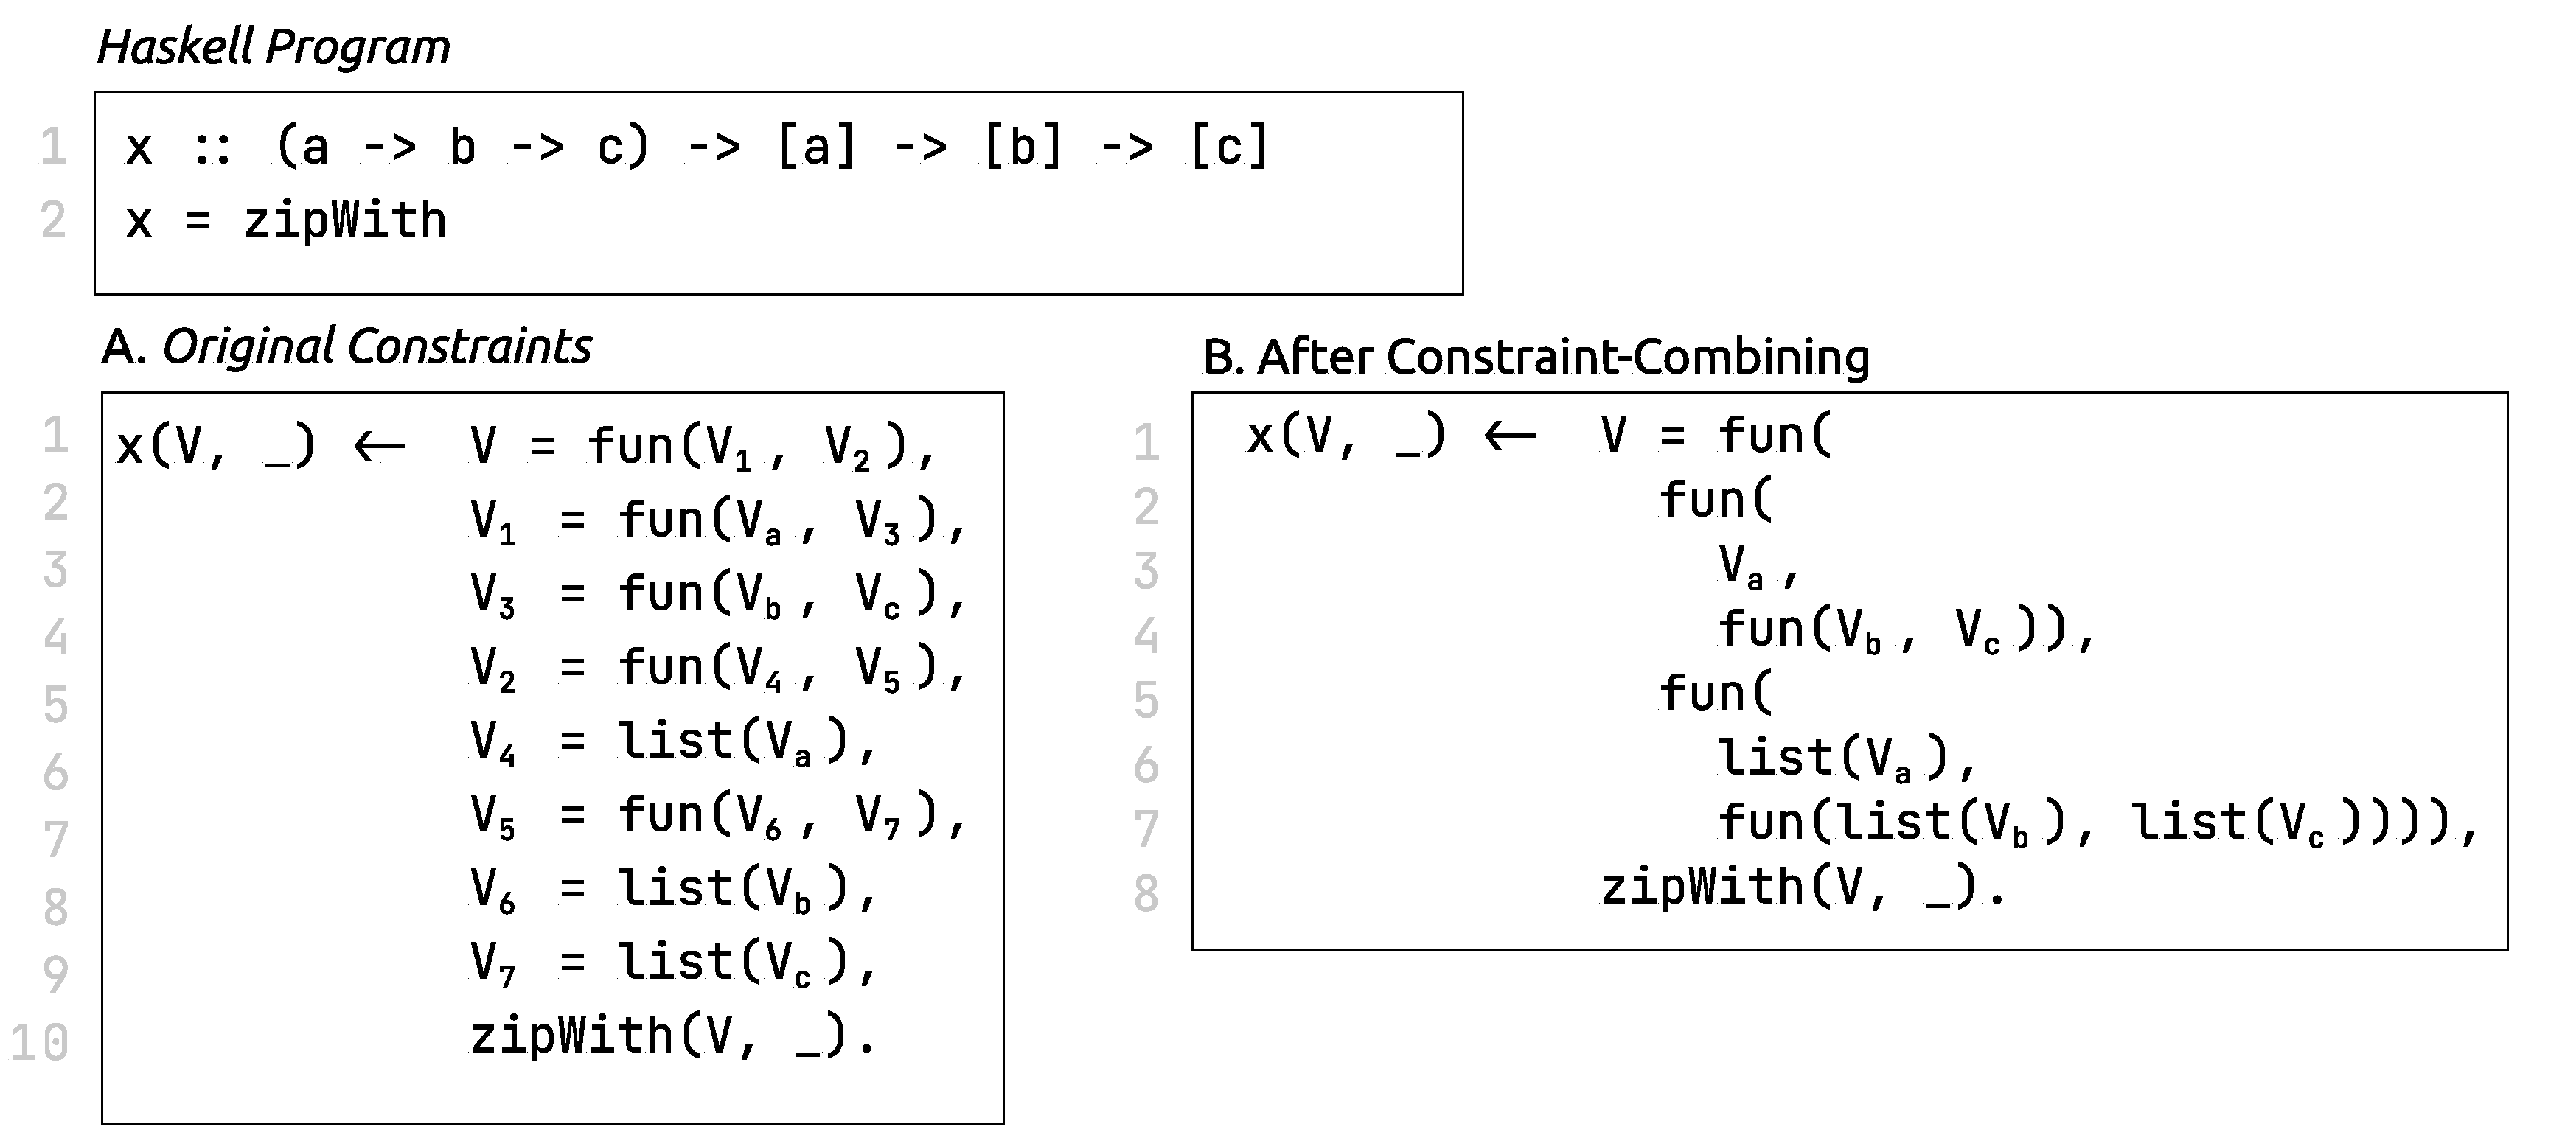
\includegraphics[width=\linewidth]{images/Combine-Constraints}
        \caption[Combine constraints in type signature]{\textbf{Combine constraints in type signature.} For a simple Haskell program (top),  without any optimization, Goanna generates 10 constraints (bottom left), indicated by 10 subgoals in the predicate. By combining the constraints in the type signature, Goanna produces 2 constraints (bottom right).}
        \label{fig:combine-constraints}
    \end{figure}

    Consider the example in Fig.~\ref{fig:combine-constraints}. Without optimization, this code would spawn 10 constraints. However, applying this optimization can achieve an equivalent outcome with merely 2 constraints. Notably, this optimization forfeits the capability to suggest fixes for sub-expressions within a type signature, a decision that warrants some consideration but, in our experience, pays off.

    \paragraph{Elimination of Over-Fitting Resolutions.}
    In general, every syntax node in the source code generates one or more constraints. This includes structural nodes such as function applications. However, very often, suggesting that the user should modify the entire function application expression is not particularly instructive when changing one of the arguments fixes the type error as well. Disabling suggestions for over-fitting solutions improves the clarity of the suggestion list and enhances the speed of MCS enumeration.
   

    \paragraph{Elimination of Redundant Causes.}
    Goanna iterates over the possible causes and removes the ones that fail to deliver new insights. If all locations in a cause suggestion have already been covered in preceding suggestions, subsequent suggestions that merely rearrange these locations in different combinations can be omitted.
    
   \begin{figure}[htb!]
        \centering
        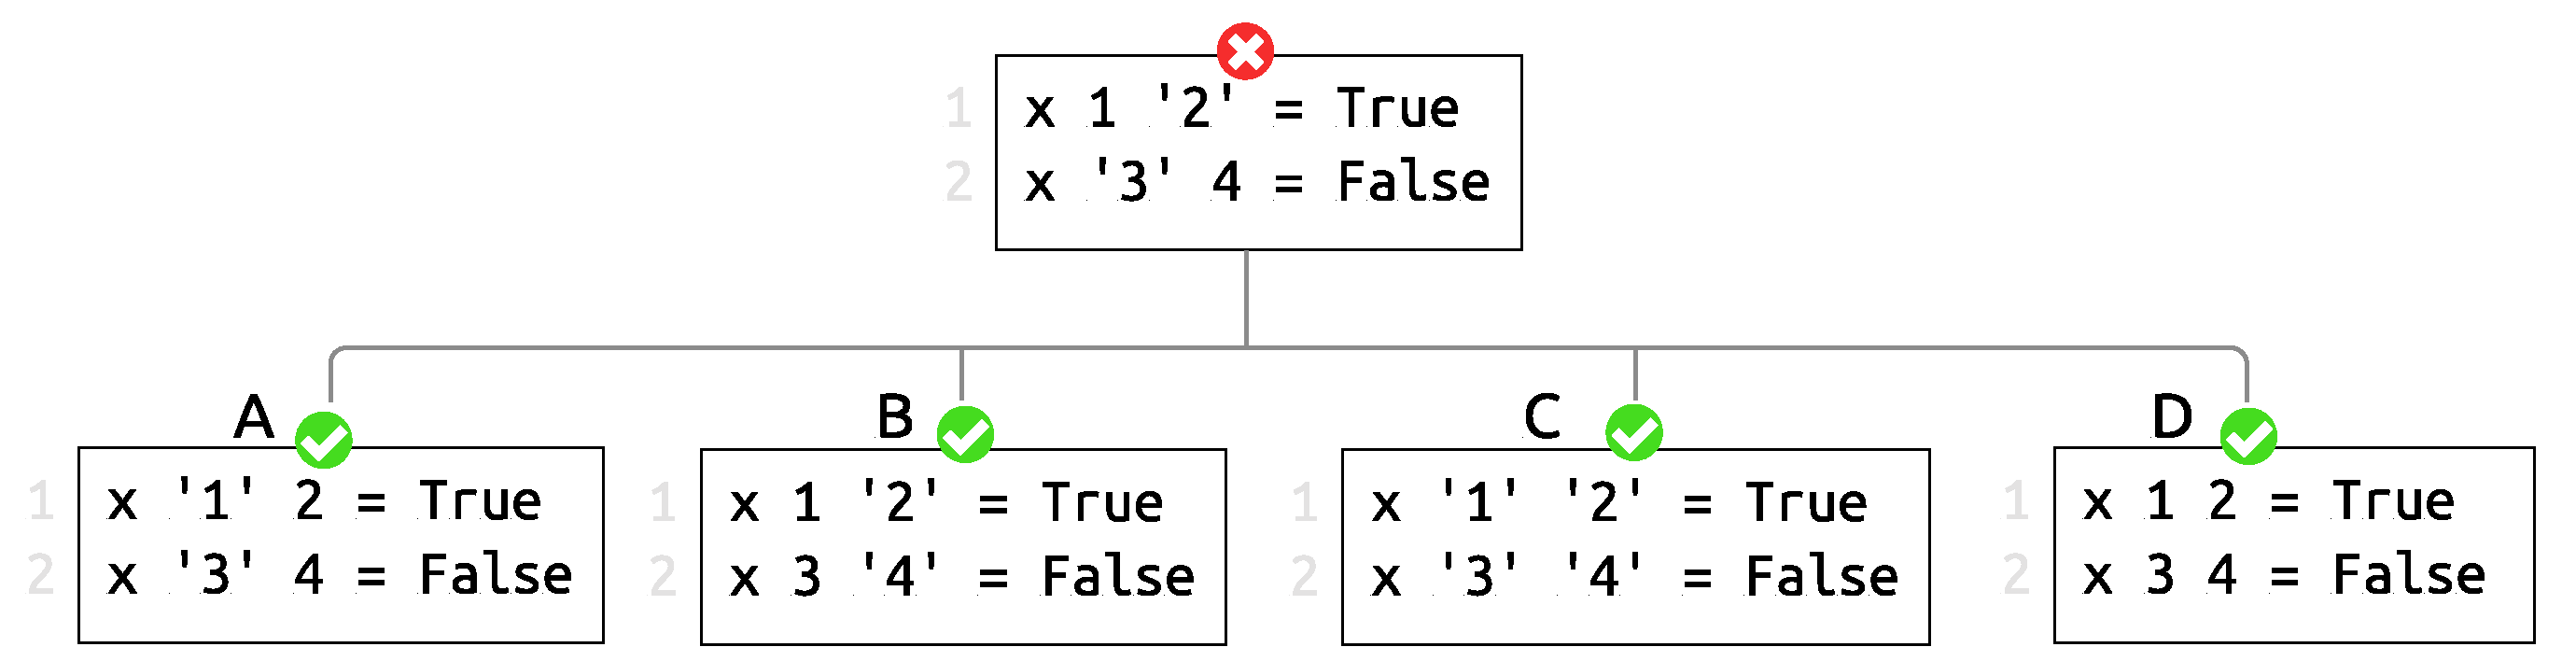
\includegraphics[width=0.9\linewidth]{images/Reduction-Example}
        \caption[The number of potential causes can grow exponentially]{\textbf{The number of potential causes can grow exponentially.} In the ill-typed Haskell program (Top), there are 4 different ways (Bottom) to fix the type error. It is not hard to see this growth is exponential, and showing all the alternatives is not helpful.}
        \label{fig:reduction-example}
    \end{figure}
    
    Consider the example in Fig.~\ref{fig:reduction-example}. Without knowing the true intention of the programmer, Goanna can provide four ways to fix the issue shown at the bottom. However, closer inspection reveals that after the first two suggestions, we no longer unearth new insights. Therefore, they can be removed to enhance the clarity of the suggestion list. 
    Note that this can remove the correct answer (say D), but if the programmer uses part of the (A) to make the fix, the revised type error will include the correct fix. 
    
    Removing superfluous MCS-based suggestions that recycle different permutations of the same set of locations is an instantiation of the Set Cover Problem (SCP). The problem can be rephrased as finding the minimal number of MCSes that cover all the potential locations that could cause the type error. Many approaches solve the SCP \cite{Caprara2000-vw}, including eager algorithms, linear programming, and heuristic-based algorithms. Generally, we found all of these approaches find the minimal cover of type errors efficiently. Goanna uses the OR-tools \cite{Google_Developers_undated-ew} for this task.
       
    \section{Evaluation} \label{sec:evaluation}

     We want to answer the following key research questions about our Goanna prototype:

    \begin{itemize}
        \item RQ1. Does Goanna provide a more accurate type error diagnosis compared to traditional tools?
        \item RQ2. Does Goanna provide a concise list of suggestions?
        \item RQ3. How efficiently does Goanna compute error diagnoses?
    \end{itemize}

    \subsection{Experiment Design} \label{sub:dataset}

    To assess Goanna, we extracted a collection of defective Haskell programs (N=86) from Haskell online discourse since 2018, each containing one or more type errors. The communities we searched include StackOverflow (32), Haskell on Reddit (20), and Haskell Discord Channel (34), as these are the top discussion channels for Haskell users \cite{Fausak2022-zf}. During the search process, we looked for online discussions where the authors encountered type errors in their Haskell programs and asked for help. Further, we selected only the questions that had been answered and accepted by the original author. We extracted the defective Haskell programs and the accepted answers as the oracle solution. The length of these programs ranges from 1 liner to 64 lines of code (mean=20, median=20). These programs span a variety of subjects, including basic syntax (14 files), lists (28 files), tuples (5 files), algebraic data types (22 files), higher-order functions (17 files), monadic operations and do notation (9 files), type classes (6 files), and built-in/library functions (24 files). The distribution of themes generally aligns with the breakdown of the different causes of the type errors from Tirronen's study \cite{Tirronen2015-nr}.
    
    	For each metric in the evaluation, Goanna is compared with Glasgow Haskell Compiler (GHC) \cite{Gamari_undated-zu}, and Helium \cite{Hage2023-kk}. GHC was chosen as the baseline due to its established reputation in the Haskell community, wide capability, and great efficiency in working with Haskell projects. Helium is acknowledged for producing high-quality error messages \cite{Heeren2003-kd}. The experiments were run with GHC 9.4 and standalone Helium compiler version 1.8.
    
    


 	\subsection{RQ1. Accuracy}\label{sub:eval-accuracy}
 	For each program in our dataset, we compared each tool's error diagnosis with the accepted answer. We consider the diagnosis accurate only if its suggested fix matches the accepted answer. We consider the diagnosis partially accurate if the tool's diagnosis is part of a larger set of locations that make up the intended cause or if the diagnosis addresses one of the multiple errors. Because Goanna provides a comprehensive list of possible causes, it is very likely all sensible fixes are included. In this evaluation, we only consider the top-1 suggestions (Goanna 1) and top-3 suggestions (Goanna 3).  From the graph in Fig.~\ref{fig:accuracy}, GHC's accuracy is the least performant among all tools. Goanna 1's, although lower than Helium (72.1\%) in partial accuracy, is higher than Helium (51.2\%) when considering only diagnoses that fully match the accepted answer. \textbf{Goanna 3 has the best accuracy (84.8\%)}, higher than the partial accuracy of other tools.
  
     \begin{figure}[htb!]
        \centering
        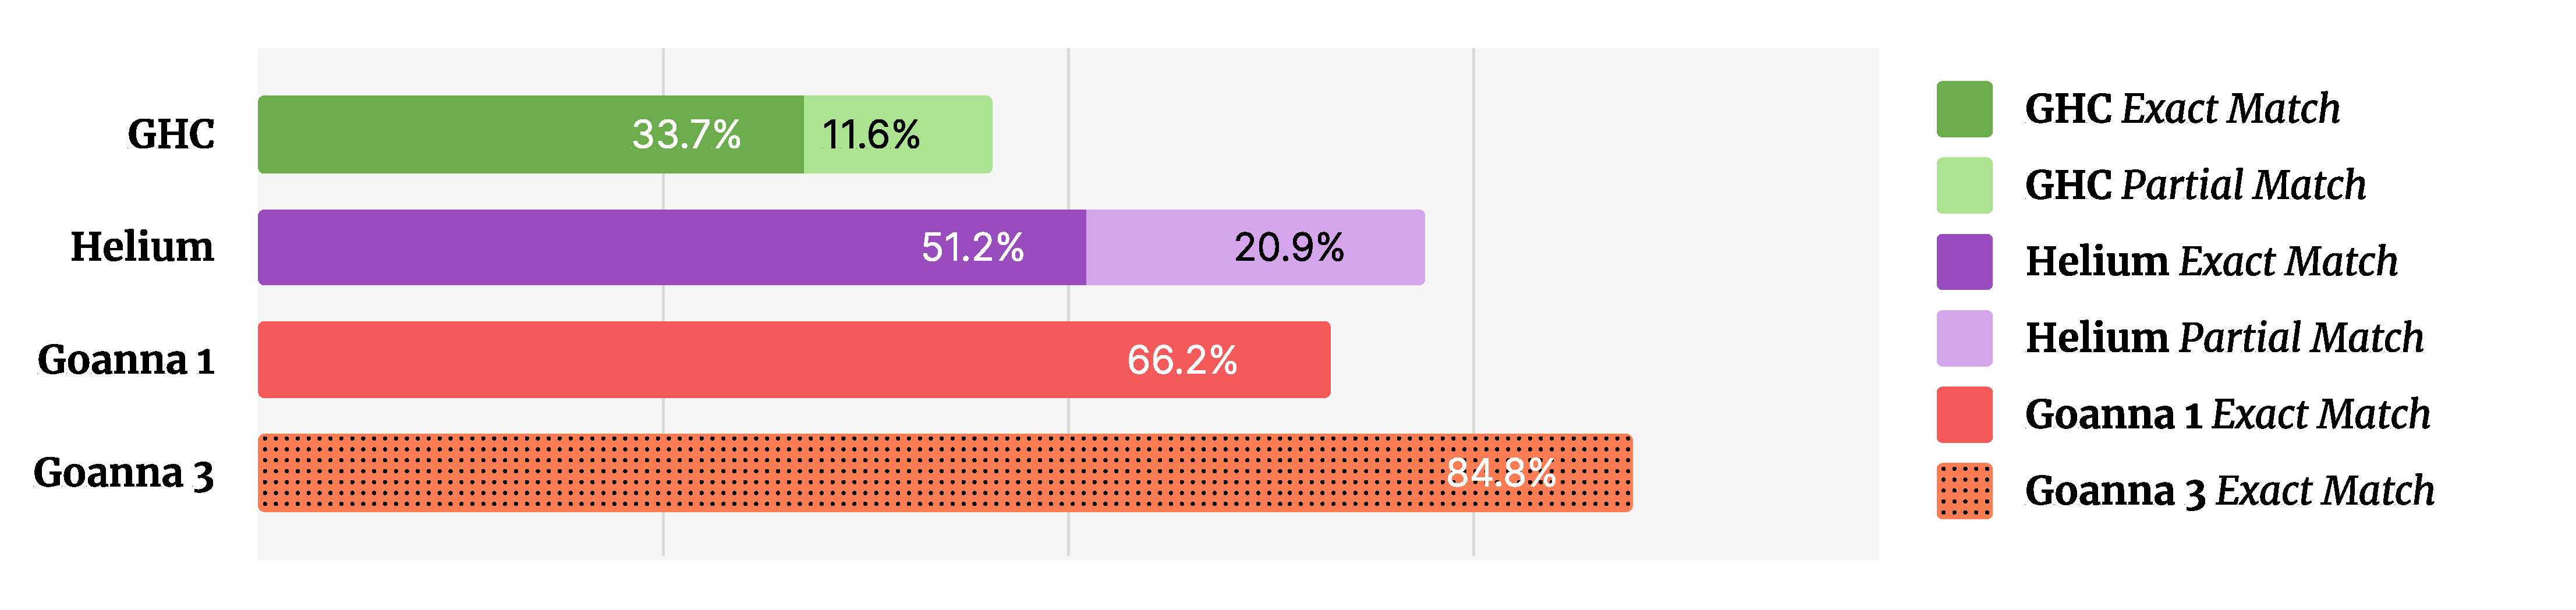
\includegraphics[width=\linewidth]{images/Accuracy}
        \caption{\textbf{The percentage of diagnoses that match the accepted answers.} }
        \label{fig:accuracy}
    \end{figure}


 	


 	\subsection{RQ2. Conciseness}\label{sub:eval-conciseness}
 Using Goanna requires users to cherry-pick from a list of possible causes. It will severely reduce the usability if the list is too long. To evaluate Goanna's conciseness, we counted the number of suggestions provided by Goanna in all the tasks.  We also indicate where the accepted answer is. Additionally, we included a baseline of Goanna with all the cause reduction features disabled. As shown in Fig.~\ref{fig:conciseness}, \textbf{Goanna manages to effectively condense its suggestion list}, on average providing a short list of suggestions (mean=3.29, median=3.0) for each type error. Additionally, on average, the accurate cause can be found within the top 2 suggestions (mean=1.63, median=1.0) to find the correct cause identification and fix. It also shows in Fig.~\ref{fig:conciseness} that Goanna's cause reduction strategies are effective; on average 51\% of total causes are reduced to gain clarity. One unusual observation is that in 3 tasks, Goanna failed to include the correct solution. The current version of Goanna is ineffective in making the correct suggestions for these type errors. We discuss this in section \ref{sec:edge-case}. 
 
    \begin{figure}[htb!]
        \centering
        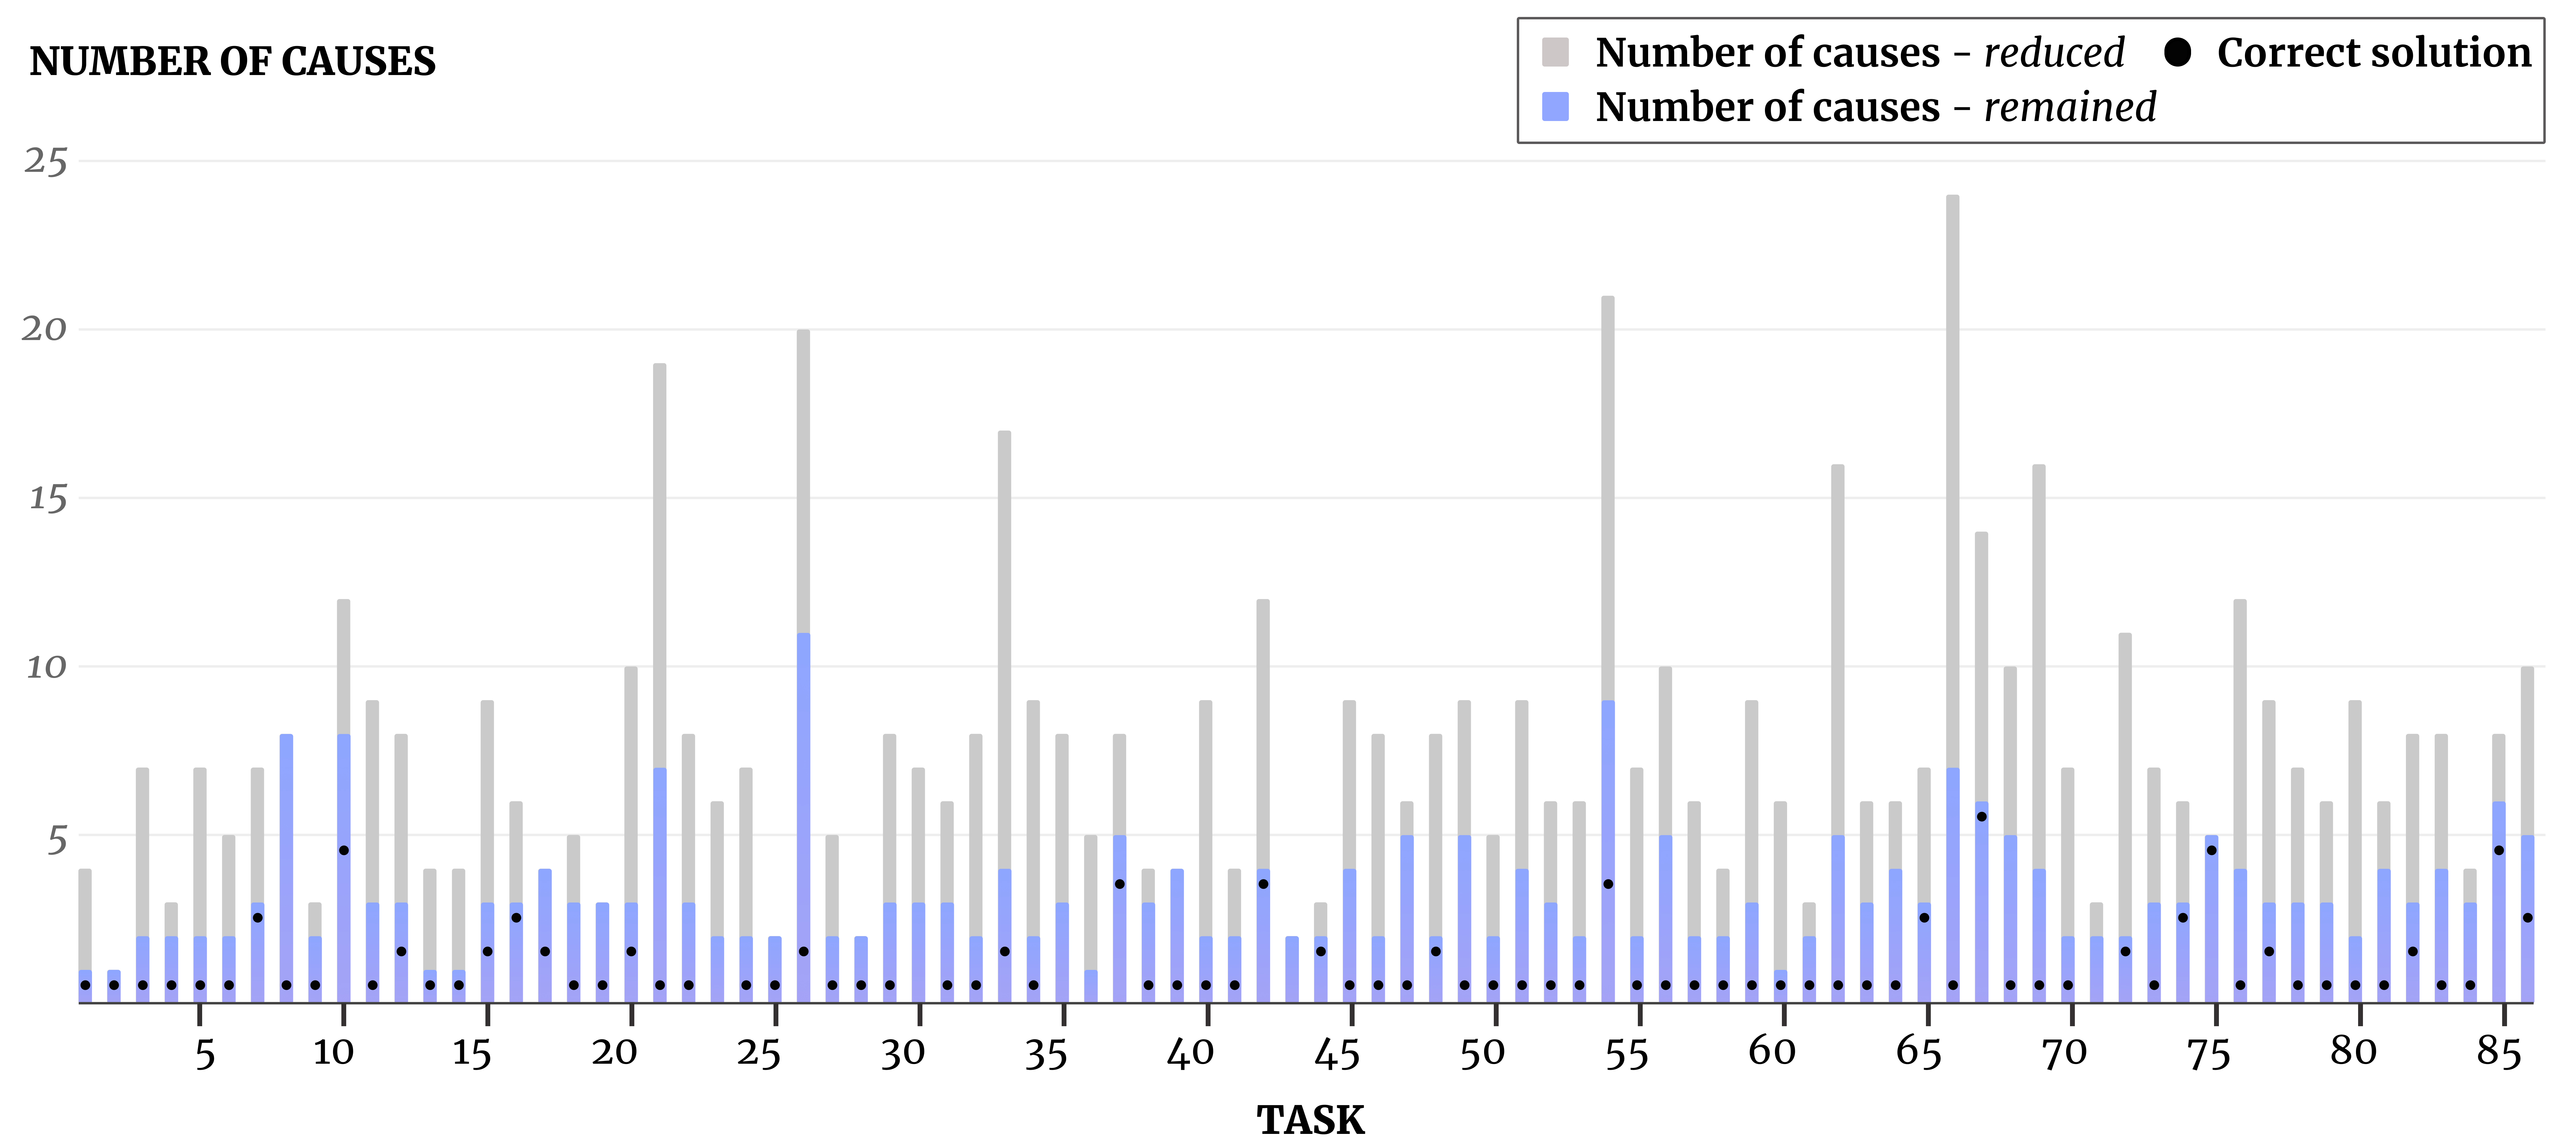
\includegraphics[width=\linewidth]{images/Conciseness}
        \caption{\textbf{The number of potential causes identified by Goanna.} }
        \label{fig:conciseness}
    \end{figure}



    \subsection{RQ3. Performance} \label{sub:eval-performacne}

    Goanna's performance largely depends on the MCS enumeration phase. Enumerating all MCS is computationally expensive. We experimentally compared the time it takes for Goanna to provide a complete error diagnosis for each task with GHC and Helium. From the data shown in Fig.~\ref{fig:performance}, we can see that \textbf{Goanna is slightly slower than Helium}~(Goanna: mean=0.98 seconds, median=0.83 seconds; Helium: mean=0.63 seconds, median=0.63 seconds). Goanna is about 10 times slower than GHC (mean=0.09 seconds, median=0.09 seconds), but greatly outperforms GHC (see Figure \ref{fig:accuracy}). One important pattern is that Goanna's response time varies more than other tools (Goanna SD = 0.55, GHC SD = 0.00, Helium SD = 0.10). It can be seen from Fig.~\ref{fig:conciseness} and Fig.~\ref{fig:performance} that the tasks Goanna struggles most with are the ones that have significantly more potential causes. Multiple avenues exist to mitigate this delay, and we will discuss them in section \ref{sec:future-work}.
    
    \begin{figure}[htb!]
        \centering
        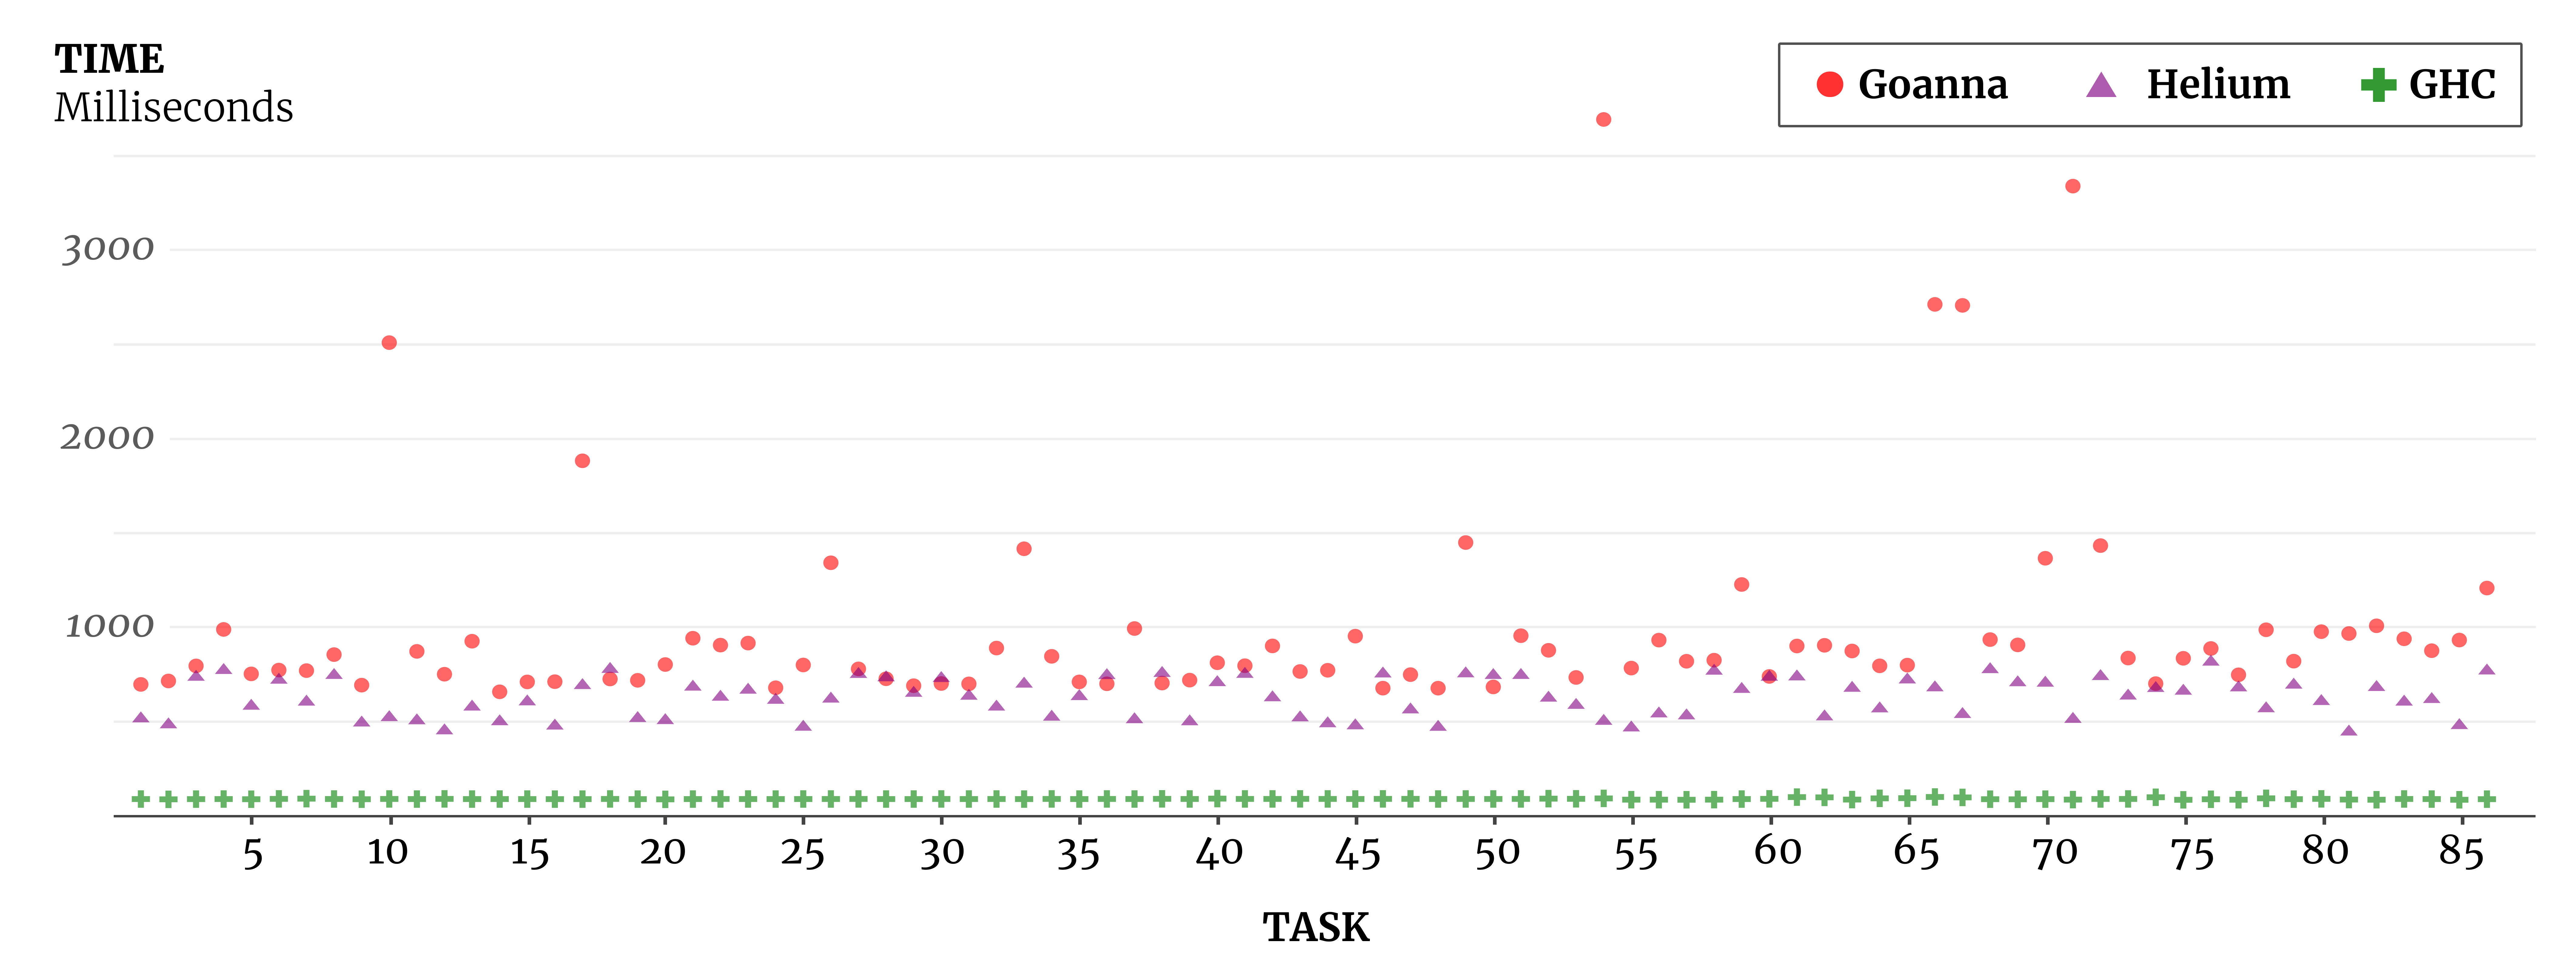
\includegraphics[width=\linewidth]{images/Performance}
        \caption{\textbf{The time it takes to type check and diagnose each program.} }
        \label{fig:performance}
    \end{figure}

	
	
% \todo{can you show a graph of some sort?}

% \todo{Any user evaluation...? Even if a preliminary one/small numnber experts would greatly help...}

% \subsection{Qualitative Results}

    \subsection{Threats to Validity}

    \paragraph{\textbf{Selection of the dataset}}
    Our selection of dataset is limited in its number. This is due to the challenge of finding programs that contain type errors. Unlike runtime errors, which can be mined from code repositories and version control histories, type errors in Haskell can be detected by the compiler tool, and ill-typed programs are usually fixed before the changes are committed to the version control systems. Further, we employed two selection methods. First, the error is indeed a type error. We test this by running the original program in GHC and checking if it indeed triggers a type error. The program is discarded otherwise, for instance, if it contains only parsing errors or runtime errors. Second, we discarded type questions where the main error relies on third-party libraries. 
    
  
        
    \paragraph{\textbf{Measurement of performance}} Performance on Goanna and GHC was measured on a Linux virtual machine with a 3.1 GHz Processor and 2GB RAM. In practice, complex systems like this may perform differently depending on hardware and software configurations. Although we were not able to extract the performance profile of each tool across different platforms and operating systems, we chose hardware with abundant resources and up-to-date software dependencies. During our performance measuring, neither CPU usage nor memory usage was fully stressed. Additionally, GHC was run with the ``-fno-code'' flag enabled to limit its usage to type-check only.


    \section{Discussion} \label{sec:discussion}

% \todo{I wonder about restructure this into strengths/limitations ; give it a bit of structure e.g. start each para with few words both/italic key finding/issue???}

    \subsection{Strengths}
    Goanna demonstrates notable improvement over existing Haskell type error detection and repair tools. Compared with traditional type-checking tools such as GHC, Goanna delivers improved error detection accuracy and flexibility to inspect different potential causes. The data suggest that users typically need to consider only 2-3 suggestions to achieve a satisfactory result. It improves error localization organization, avoiding the presentation of all error locations at once.


    \paragraph{\textbf{Accurate suggestions}} Goanna is able to identify causes for Haskell type errors more accurately than GHC and Helium. We attribute this to a few factors. First, Goanna is the only tool capable of suggesting the type error in more than one node. In a study~\cite{Wu2017-eb} of over 2700 ill-typed Haskell programs, only 35\% of the type errors were caused by a single location. However, most of the type debugging tools only focus on single-location causes due to their technical limitation or to avoid high computational cost. Second, Goanna is the only tool that provides alternative causes of a type error. We were able to see that although Goanna-1 is not as accurate as Helium when accepting partial fixes, Goanna-3 surpasses Helium in accuracy. This translates into accurate type error identification at the cost of presenting the top 3 answers from Goanna instead of one.
    

    \paragraph{\textbf{Goanna provides contextual information}}
    Goanna provides type information for relevant terms to support each of its claimed causes. In traditional tools, the type-level information is often incomplete or totally discarded. In runtime error debugging, one of the most common features is inspecting the values of different expressions of the program. It would be ineffective if the runtime debugger only showed the location of the error. Goanna simulates this feature in the type debugging setting. Instead of run-time values, Goanna allows programmers to inspect the type assignments and observe how they change with different assumptions of the potential cause of a type error. 

    \subsection{Weaknesses}

    \paragraph{\textbf{Responsiveness}}
    The trade-off of extensive analysis undertaken in Goanna results in a substantial delay (mean=0.98s).
    The current performance of Goanna is not yet suited for real-time feedback in programming tasks. Based on Nielsen's suggestion for wait time tolerance \cite{Ferdowsi2023-au}, Goanna should provide responsive answers ($\leq$ 1 second) for real-time programming analysis, where users' flow of thoughts stays uninterrupted. Even in larger and more complex tasks, Goanna's response time ($\leq$ 10 seconds) is still suitable as an on-demand tool when a complex type error occurs. As shown in Wu's study \cite{Wu2017-eb}, in the simplest situation where students fix the type error in a single step, it will usually take about 60 seconds to complete the task. This error resolution time grows in proportion to the number of steps the students take to fix the error. If Goanna is able to shorten the steps to final resolution, then the querying time will easily be offset by the time it saves.

    \paragraph{\textbf{Edge cases}} \label{sec:edge-case}
    Although Goanna's error reporting is, in general, exhaustive, there are situations where Goanna still fails to provide insightful diagnosis. One general theme is that Goanna is very effective when the error requires modifying a syntax node but can be less insightful when the intended fix is to insert, delete, or rearrange syntax nodes. In the example in Fig.~\ref{fig:weakness}, Goanna suggests changing the \texttt{map} function to a function of type \texttt{[Int] -> [Bool]}. But in practice, a human user would very easily identify that an expression defining the function to be mapped is missing between the map and the list being operated on.
    
        \begin{figure}[htb!]
        \centering
        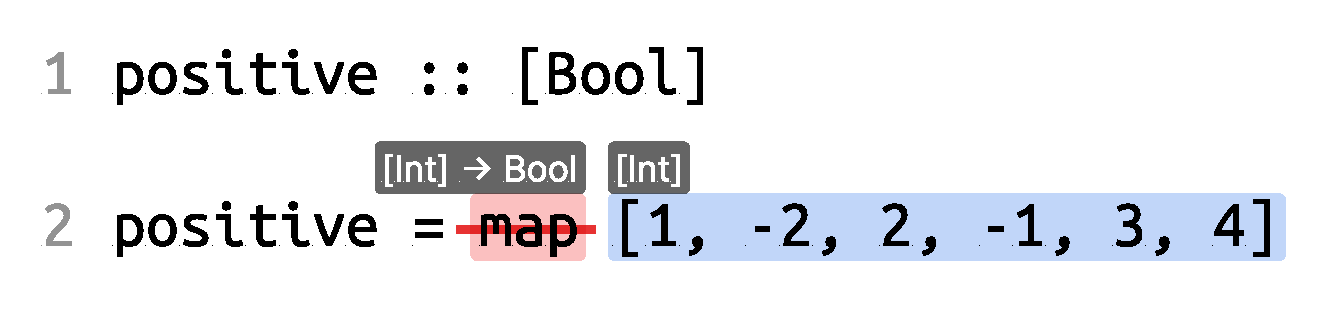
\includegraphics[width=0.6\linewidth]{images/Weakness}
        \caption[Edge cases in Goanna]{\textbf{} In this type error, Goanna suggests changing \texttt{map} to a function of type \texttt{[Int] -> Bool}. Although this is technically correct, in practice, a human expert user would easily identify that a function expression is missing between the function \texttt{map} and the list literal.}
        \label{fig:weakness}
    \end{figure}

%    \paragraph{\textbf{Goanna's suggestions are local}}
%    One potential argument against Goanna's method is its tendency to generate local changes for fixes. Some consider that errors sometimes demand architectural changes rather than localised adjustments. To address this concern, Goanna implements two strategies. Firstly, Goanna presents all relevant error locations in style similar to type error slicing tools and reports all definitions and usages related to a type error. These hints can serve as a mental map to guide the formulation of changes on a large scale and understand their implications at the source code level. Secondly, Goanna consistently provides potential changes in type annotations. A top-level type annotation is a common approach for programmers to map out high-level structures at various stages of Haskell projects. Understanding the required changes at this level enables programmers to adopt a more principled development approach.
%
%	
%	\subsection{Implication}
%	Goanna shows a novel approach to model type errors, and enhances our ability to interrogate them.  Goanna also shows various type error optimization and enhancement opportunities enabled by constraint programming techniques. It suggests more useful programming languages and tools can be developed equipped with MCS-based analysis.
	



% \subsection{Different Category of Type Errors}
% \subsubsection{Where are all the materials}
% \subsubsection{Type errors that involve a long chain of reasoning}
% This kind of type error tend to cause Goanna to report a large number of suggestions. This is easy to understand intuitively because in a long chain of reasoning, breaking any one of them will result in a valid program. So the number of solution should be in propotion to the length of the chain.

\subsection{Future Work}\label{sec:future-work}
  	It is important to evaluate Goanna with human participants  and gain qualitative insight of its effectiveness. In  one of our workshop preliminary study, participants show positive reaction after using Goanna. A rigorous human study based on realistic debugging use cases is planned in the near future.   
  	
  	
    Several areas of potential enhancement could improve Goanna's functionality and efficiency. One exciting path of improvement is to generate suggestions for syntax changes on top of type changes. As pointed out in \cite{Chen2014-dz}, syntax changes are much more challenging. But with the recent improvements of generative models and research advancement in ML-based type error \cite{Seidel2017-uf}, accurate syntax change may be on the path to becoming feasible.

    Several approaches to achieve higher performance of Goanna show promise. The parallel capability of state of art MUS enumeration \cite{Zhao2016-bu} algorithms are not explored in this study. With proper implementation, it will be possible to lower the hardware barrier of entry for wide adoption of MCS-based type error suggestion tools. Further, with domain-agnostic MUS enumeration tools \cite{Bendik2020-pz}, it should be possible to consistently achieve high performance while using a more performant constraint system and proper parameterization. Lastly, in a real-world implementation, it is possible to employ partial MUS enumeration \cite{Previti2013-mr,Liffiton2016-xi} to restrict the enumeration process in a sensible time-bound.

    Additional future work could include examining Goanna's integration with other tools within the Haskell development ecosystem. For instance, include Goanna in widely used text editors or development environments could offer a more integrated and fluid experience for developers, and an important avenue for Goanna to reach a wider audience. 

    Finally, it may be important to consider extending Goanna's capabilities to support other functional programming languages beyond Haskell. Several other languages, including Scala and OCaml, also support static typing and type inference, and Goanna could be a valuable addition in these contexts. In future, we also hope to extend these techniques to popular multi-paradigm languages such as TypeScript and Rust.


    \section{Related Work} \label{sec:related-work}
	\subsection{MCS enumeration}
	
    MCS enumeration has been extensively studied in the field of error localization across various domains. In the specific context of Haskell type error diagnosis and resolution, several related approaches have been explored. It is important to examine the strengths and weaknesses of Goanna in the context of these areas.

    One notable work by Lamraoui et al. introduced a tool \cite{Lamraoui2016-wr} that utilizes the capability of MCS to localize multiple faults and identify software defects using unit tests. Their approach demonstrated the effectiveness of MCS in pinpointing errors within a program. Similarly, Bekkouche et al. conducted a relevant study  \cite{Bekkouche2015-is}  on MCS utilization for locating program errors in while-loop programs. Their findings showed improved efficiency compared to SAT-based approaches. Although showing strength in programming language static analysis, MCS-based fault localization has not been previously applied at the type system level. Goanna distinguishes itself as the first tool to explore this approach within the realm of type error diagnosis and resolution.

    \subsection{Suggesting changes to type errors}
   Lerner et al. proposed Seminal \cite{Lerner2007-mu}, using syntax mutation and binary search to find appropriate syntax changes to program errors. The advantage of Seminal is that it's capable of suggesting direct syntax changes to common mistakes (e.g. mistakingly swapped the order of function arguments). However, it is impossible for Seminal to provide the complete set of all potential fixes. Nor does it guarantee a suggested sulution is minimal syntax change.
   
   Counter-factual typing (CFT) \cite{Chen2014-dz,Chen2020-ad} uses variation-based type system; it is capable of suggesting the correct type for all possible. CFT shares many capabilities with Goanna, CFT is able to suggest multiple-location changes, CFT uses similar ranking heuristics. Goanna is able to produce in-depth analysis of the ill-type program, such as type error isolation. CFT and Goanna both aim to produce a complete set of potential fixes, Goanna employs a set of effective algorithms to reduce the exponential number of potential fixes without suffering the quality of suggestions. 
   
   SHErrLoc \cite{Zhang2015-xy} uses constraints as the underlying to perform type inference and type error diagnoses. SHErrLoc is able to suggest multiple possible fixes of the type error and rank them based on heuristics. Unlike Goanna's approach of using a general purpose constraint language, SHErrLoc relies on GHC's internal constraints and then translates them into SCL (a custom-made constraint language). On technical side, this approach relies heavily on modification of the compiler and does not remain reliable with later GHCs. Most importantly, there is no way to directly interact with the solver. This renders the kind of constraint manipulation in Goanna and SHErrLoc impossible. Goanna is able to perform type reconstruction for ill type programs, that is, finding the most concrete types for all expressions for each potential solution using the Maximal Satisfiable Subsets. SHErrLoc focuses on finding the locations only.


\subsection{Type Error Slicing}

Type error slicing \cite{Haack2004-fr} is a technique to identify all necessary locations of a type error that is necessary for programmers to diagnose the root cause. It has been studied in many studies ever since \cite{Tip2001-qn, Heeren2003-kd}. These studies all use Minimal Unsatisfiable Subset (MUS) to ensure the \textit{completeness} and \textit{minimality}. The drawback of type error slicing is that it often produce too many locations.  Chameleon \cite{Stuckey2003-pz,Fu2021-xd} improved type error slicing by allow programmers to interactively show the partial MUS by choosing their own assumptions. Compared to these tools that base their analysis on a single MUS, Goanna effectively utilizes all possible MUSes. This allow Goanna to enhance its suggestions based on the improve knowledge of the underlying type error. For example, it uses the number of MUSes a location appears in to rank how likely the location is part of the root cause. This is not possible with a single MUS.  
%   
%   This type-based approach aims to provide more accurate and meaningful suggestions for resolving type errors. Goanna falls into the latter category, offering type-based suggestions. However, it is important to note that while Chen's approach relies on search-based techniques, Goanna utilizes the MCS as the underlying suggestion representation. This gives Goanna the advantage of providing resolutions that change multiple syntax nodes in a single fix suggestion. Additionally, using MUS enumeration allows Goanna to perform high-level type error diagnoses, such as effectively identifying the number of type errors present and logically grouping them in intuitive partitions.

%    Constraint-based typing rule translation has been exercised in multiple studies. For instance, \cite{Stuckey2003-pz,Fu2021-xd} demonstrated how to translate Haskell typing relations into constraint-handling rules for improved error reporting. Their work aimed to enhance the understanding and identification of type errors by leveraging constraint-based techniques. Similarly, Demoen et al. \cite{Demoen1999-oj} presented an approach for translating Mercury typing constraints into Prolog formulae similar to Goanna's constraint translation system. These studies have shown the potential of constraint-based type systems in providing explainable and diagnostic capabilities. However, many of these works focus on type system modeling and error reporting based on a single MUS, mainly because they were conducted before efficient MUS/MCS enumeration became practical. In contrast, Goanna effectively utilizes all possible MUSes, providing a complete picture of the error and offering enhanced organizational capabilities for better error diagnosis and resolution.
%
%    By analyzing the existing literature on MCS enumeration, type error fix suggestions, and constraint-based typing rule translation, we can gain valuable insights into the distinctiveness of Goanna's approach. Goanna not only explores MCS enumeration in the context of type error diagnosis and resolution but also provides type-based suggestions and leverages the power of constraint-based techniques to offer comprehensive and intuitive error explanations and resolutions. These contributions position Goanna as an innovative tool with the potential to enhance the development process and improve the productivity of Haskell programmers.


    \section{Summary} \label{sec:conclusion}
    In this paper, we introduced Goanna, a tool for identifying and resolving type errors in Haskell code. We described the features of Goanna, including its fix suggestions, type error grouping, and identifying multiple type errors. We also discussed our approaches to reduce and reprioritize fix suggestions while maintaining comprehensiveness. Additionally, we walked through the uses of Goanna-IDE, a type error debugging interface for Haskell.

    We evaluated the effectiveness of Goanna from a set of 86 diverse Haskell programs and demonstrated its ability to identify and resolve type errors accurately compared to other tools. We also showed that Goanna effectively condenses the list of causes. When a large number of causes is inevitable, Goanna's suggestion ranking heuristics ensures that more useful fixes are prioritized. Goanna currently works with Haskell, but in the future, we plan to extend its MCS-based error diagnosis to work with other strongly typed languages.
     


% Chapter 5

\chapter{A Diagrammatic Notation for Haskell Types}

\label{chapter5} 


\section{Motivation Example}

\section{Feature Walkthrough}

\section{Evaluation}

\section{Conclusion and Future Work}


% Chapter 6

\chapter{Future work: An Integrated Debugging Framework}\label{chap:future-work} 

\section{A Design of The Integrated Debugging Framework}

\section{Debugging Features}
\subsection{Finding and Explaining Potential Causes}

\subsection{Finding Syntax Changes with Graphic Notation}

\subsection{Identify 4 Types of Potential Fixes With Graphical Comparison}

 \begin{figure}[htp]
        \centering
        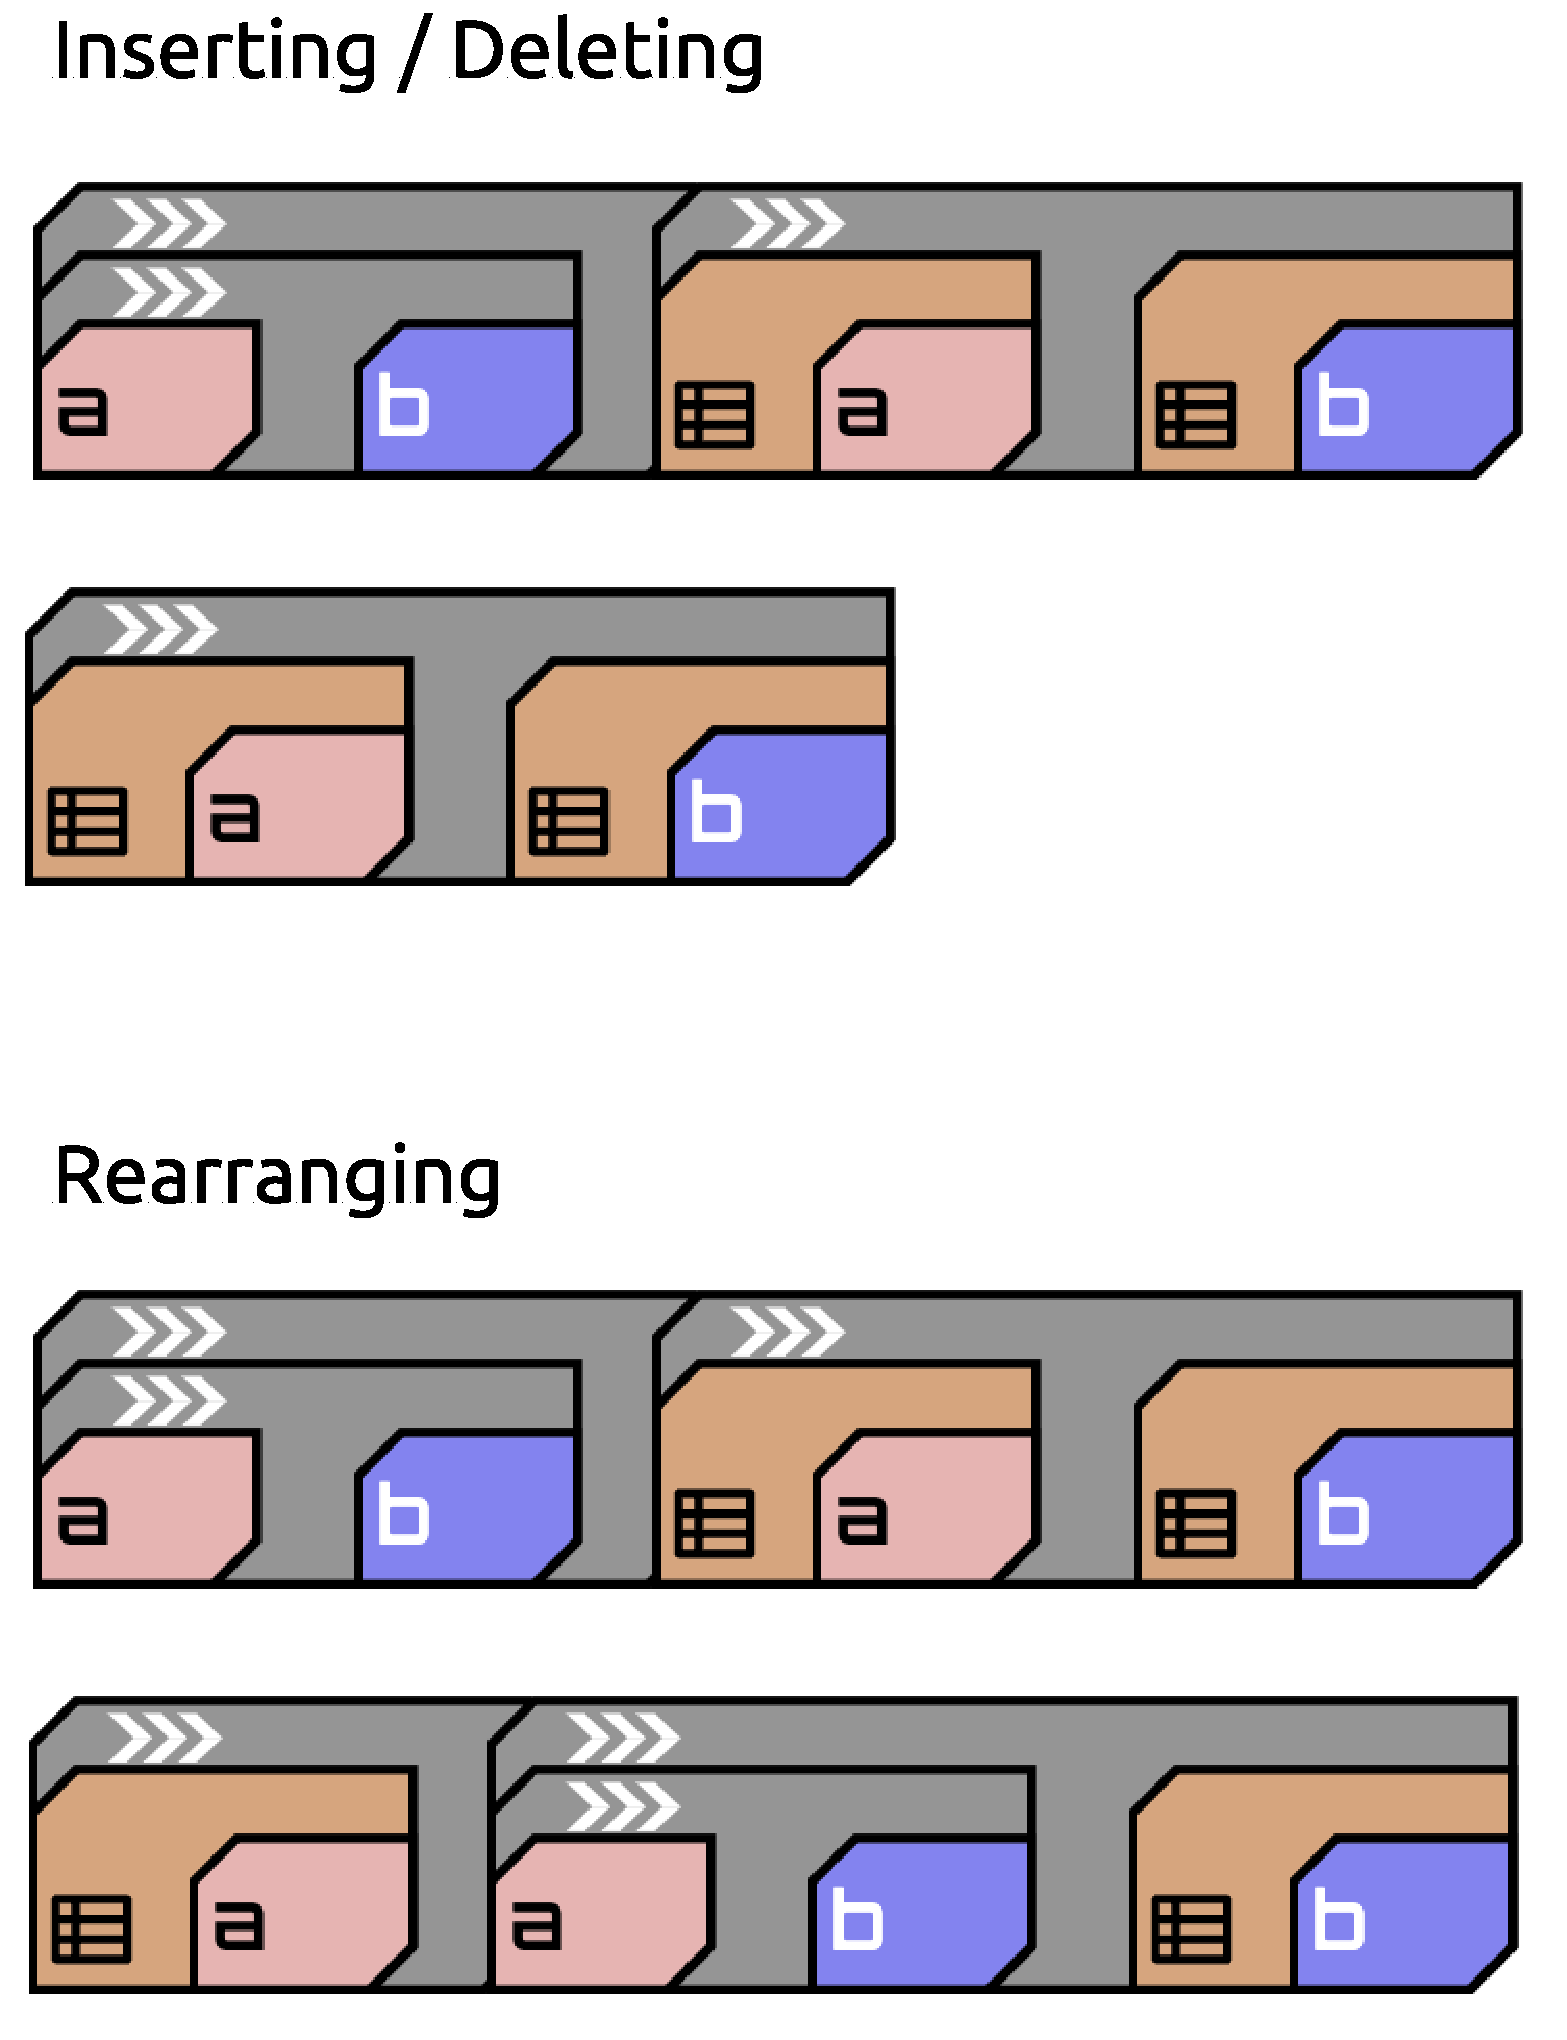
\includegraphics[width=0.5\linewidth]{Figures/TypesOfCauses}
        \caption{Different Types of Potential Fixes}
        \label{fig:type_of_fix}
    \end{figure}

\paragraph{Inserting to Fix}
\paragraph{Deleting to Fix}
\paragraph{Modifying to Fix}
\paragraph{Rearranging to Fix}

\section{Walkthrough}


\section{Discussion}


\section{Conclusion}



\chapter{Conclusion}

\label{chap:conclusion} 
\newcommand{\typetutor}{TypeTutor}

\graphicspath{{Figures/Conclusion}}
At the beginning of this thesis, we gave an overview of the landscape of programming languages, with a special interest in functional programming and static typing. We emphasized the critical role of type errors, noting how problematic type errors can hinder both the learning and the effective use of statically typed languages. Then, we explored various Haskell type-checking methods and their evolution, setting the stage for an in-depth discussion of our interventions, \chameleon{}, Goanna, and GeckoGraph, which are designed to deliver accurate and user-friendly error messages.

In this chapter, we review our contributions and discuss the future work that builds upon these initiatives. The planned future work encompasses what we consider a natural next step in tool design, integration with large language models (LLMs), and language availability. We provide detailed visions for how debugging type errors can be further improved using our acquired knowledge. We conclude our discussion by reaffirming our commitment to improving type errors, a core objective of this thesis, and reiterating the importance of this work within the broader field of programming language research.


\section{Contributions}

In this thesis, we present four key areas of contribution: a categorization of type errors, \chameleon{}, Goanna, and GeckoGraph. 

\subsection*{A categorization of type errors}


We have developed a categorization framework for type errors based on insights from how human programmers perceive type errors and theories from constraint satisfiability research. This framework helps identify three critical attributes of type errors, enhancing our understanding of strategic interventions to assist programmers in resolving these errors effectively.

\begin{itemize}
    \item {\textbf{Multi-step type errors} These errors involve a sequence of logical deductions, requiring programmers to look for multiple locations of the source code to forge a coherent reasoning chain. It is crucial to clearly present these locations and their interconnected relationships within the source code to streamline this reasoning process.}
    \item{\textbf{Multi-witness type errors}  These errors present an imbalance in the evidence, leading to two possible causes. Highlighting this discrepancy can guide programmers toward a more informed evaluation of the likely root causes, aiding in quicker resolution.}
    \item{\textbf{Multi-party type errors} These errors involve conflicts that present more than two potential possible types. They often indicate the coexistence of multiple underlying errors. Providing tools that can break down these errors into multiple type errors of simpler form allows programmers to tackle each error sequentially, leading to a simpler debugging workflow.}
\end{itemize}


Following this classification, we delved into the three main systems we developed in our research:\chameleon{} (see Chapter \ref{chap:chameleon}), Goanna (see Chapter \ref{chap:goanna}), and GeckoGraph (see Chapter \ref{chap:gecko-graph}). Each system is designed to tackle some different challenges associated with debugging type errors.

\subsection*{Explain Multi-step type errors and the chain of thought visualization}


We introduce \textbf{\chameleon{}}, an interactive Haskell type error debugging tool. \chameleon{} uses Minimal Unsatisfiable Subsets (MUS) as its core type error representation. Our work on \chameleon{} is based on the existing work on Chameleon \cite{Stuckey2003-pz, Wazny2006-ll}. The original Chameleon was developed as a command-line tool; its innovative approach of interactive debugging allows programmers to view different possible type error explanations and type assignments by issuing console commands.  We took the idea of an MUS-based Haskell debugging tool and interactive debugging techniques and provided a modern implementation with many advanced features. Notably, \chameleon{} enables programmers to explore the chain of reasoning behind type errors in step-by-step order. Additionally, \chameleon{} features an adaptive user interface, allowing programmers to tailor the information density of type errors according to their experience level.


We conducted three user studies to investigate the impacts of using debugging tools that support type error slicing and interactive type error exploration, some key features provided in \chameleon{}. Our findings reveal a notable improvement in debugging speed when employing the type error-slicing technique, particularly for complex tasks. Additionally, across the experience level, we observed a significant enhancement in debugging speed when programmers engaged with the interactive debugging features, suggesting that active exploration of type errors can positively impact the debugging process.

\subsection*{Resolve multi-witness and multi-party errors with Minimal Correction Subsets}

We contribute \textbf{Goanna}, a Haskell type error debugging tool that, like \chameleon{}, utilizes type error slicing to achieve comprehensive and user-friendly error localization.

Goanna sets itself apart by employing Minimal Correction Sets (MCS) to identify potential causes of type errors. It conducts an exhaustive analysis of all potential causes and corresponding actions required to resolve the type error. In addition, Goanna employs a set of heuristics to avoid an overwhelming list of suggestions. These heuristics filter out less useful suggestions and prioritize potential causes based on their likelihood, ensuring a more focused and effective debugging experience.


To assess the efficacy of MCS-based type error debugging strategies, we compiled a dataset of 86 Haskell programs sourced from various online discussions, embodying a wide range of type error scenarios. We evaluated the accuracy of Goanna in identifying and resolving type errors in comparison to traditional compiler tools. Our findings affirm that Goanna consistently provides more accurate error-cause identification compared to other tools. Further, our heuristics not only effectively narrow down the list of possible causes but also consistently include the real cause in its top recommendations. Lastly, although Goanna is slower than the conventional tools, it remains well within a range suitable for providing real-time feedback. 

\subsection*{Visualizing Types}

We introduce \textbf{GeckoGraph}, an innovative graphic notation system designed specifically for Haskell types. Unlike traditional type signatures, GeckoGraph utilizes a combination of colors, shapes, and symbols to highlight distinct type structures. GeckoGraph provides a clear visual representation for type-level features such as type classes, parametric type variables, and high-rank types. When programmers need to compare two types, a frequent requirement in resolving type errors, GeckoGraph provides strong visual grouping that is often able to underscore subtle differences, providing clear graphical distinctions.

We conducted a large-scale user study to evaluate the effectiveness of GeckoGraph in enhancing the traditional text-based approach to type signatures. The study was designed as an interactive puzzle game incorporating gamification elements to stimulate participation and engagement. In total,  721 programmers of all experience levels participated in the study. While the results showed that the use of GeckoGraph did not significantly impact the speed or overall success rate of solving problems, it proved significant in supporting beginners in solving harder tasks more successfully. Additionally, feedback collected through a qualitative post-study survey was positive, suggesting that GeckoGraph is intuitive, non-intrusive, and helpful.

\section{Future Work}

In this section, we present three promising directions stemming from our existing work. Firstly, drawing upon our prior experience of researching type debugging tools, we now sketch a novel debugging tool: \textit{TypeTutor}. We envision the interfaces and interactions within \textit{TypeTutor}, which have been shaped by insights from our existing tools and feedback from various user studies.

Secondly, we delve into the realm of rapid advancements in large language models (LLMs) and their evolving role in programming assistance, distinguishing them from conventional theory-based tools like \chameleon{} and Goanna. We explore the possibility of integrating traditional tools with LLMs to effectively capitalize on their unique strengths and address their weaknesses.

Lastly, we outline our plans to adapt our debugging tools for use in other programming languages, underscoring the potential advantages and challenges associated with this endeavor.

\subsection*{\typetutor: Question-Based Type Debugging}

By observing programmers tackle type error challenges in a series of user studies, we gained valuable insights into Haskell programmers' debugging habits and approaches toward challenging type errors. Armed with this understanding, we are inspired to envision a novel debugging tool named \textit{TypeTutor}. The core concept of \textit{TypeTutor} would be to map debugging tasks into a series of questions that programmers would naturally ask, while also to help programmers break down high-level debugging questions into actionable, granular queries.

This style of programming is often referred to as ``natural programming environment'' \cite{Myers2004-fy}. Previous studies have underscored the benefits of employing a natural debugging interface, exemplified by tools such as Alice~\cite{Conway2000-nn} and WhyLine~\cite{Ko2009-uf}. However, existing research predominantly concentrates on debugging runtime errors, neglecting exploration into type-level debugging.  Leveraging our experience with \chameleon{}, Goanna, and GeckoGraph, we envision meaningful progress in this domain.


\subsubsection*{Why questions}

A fundamental aspect of debugging type errors involves asking questions such as "Why does the type error occur?" and "Why is the expected type \texttt{X}?" These "why" questions highlight gaps in understanding where a thorough explanation is in demand. \textit{TypeTutor} will intelligently address this by displaying all relevant "why" questions when a programmer hovers over an expression of interest. Upon selecting a question, \textit{TypeTutor} will promptly provide the corresponding detailed answer (Fig.~\ref{fig:why}).



\begin{figure}[hbt]
  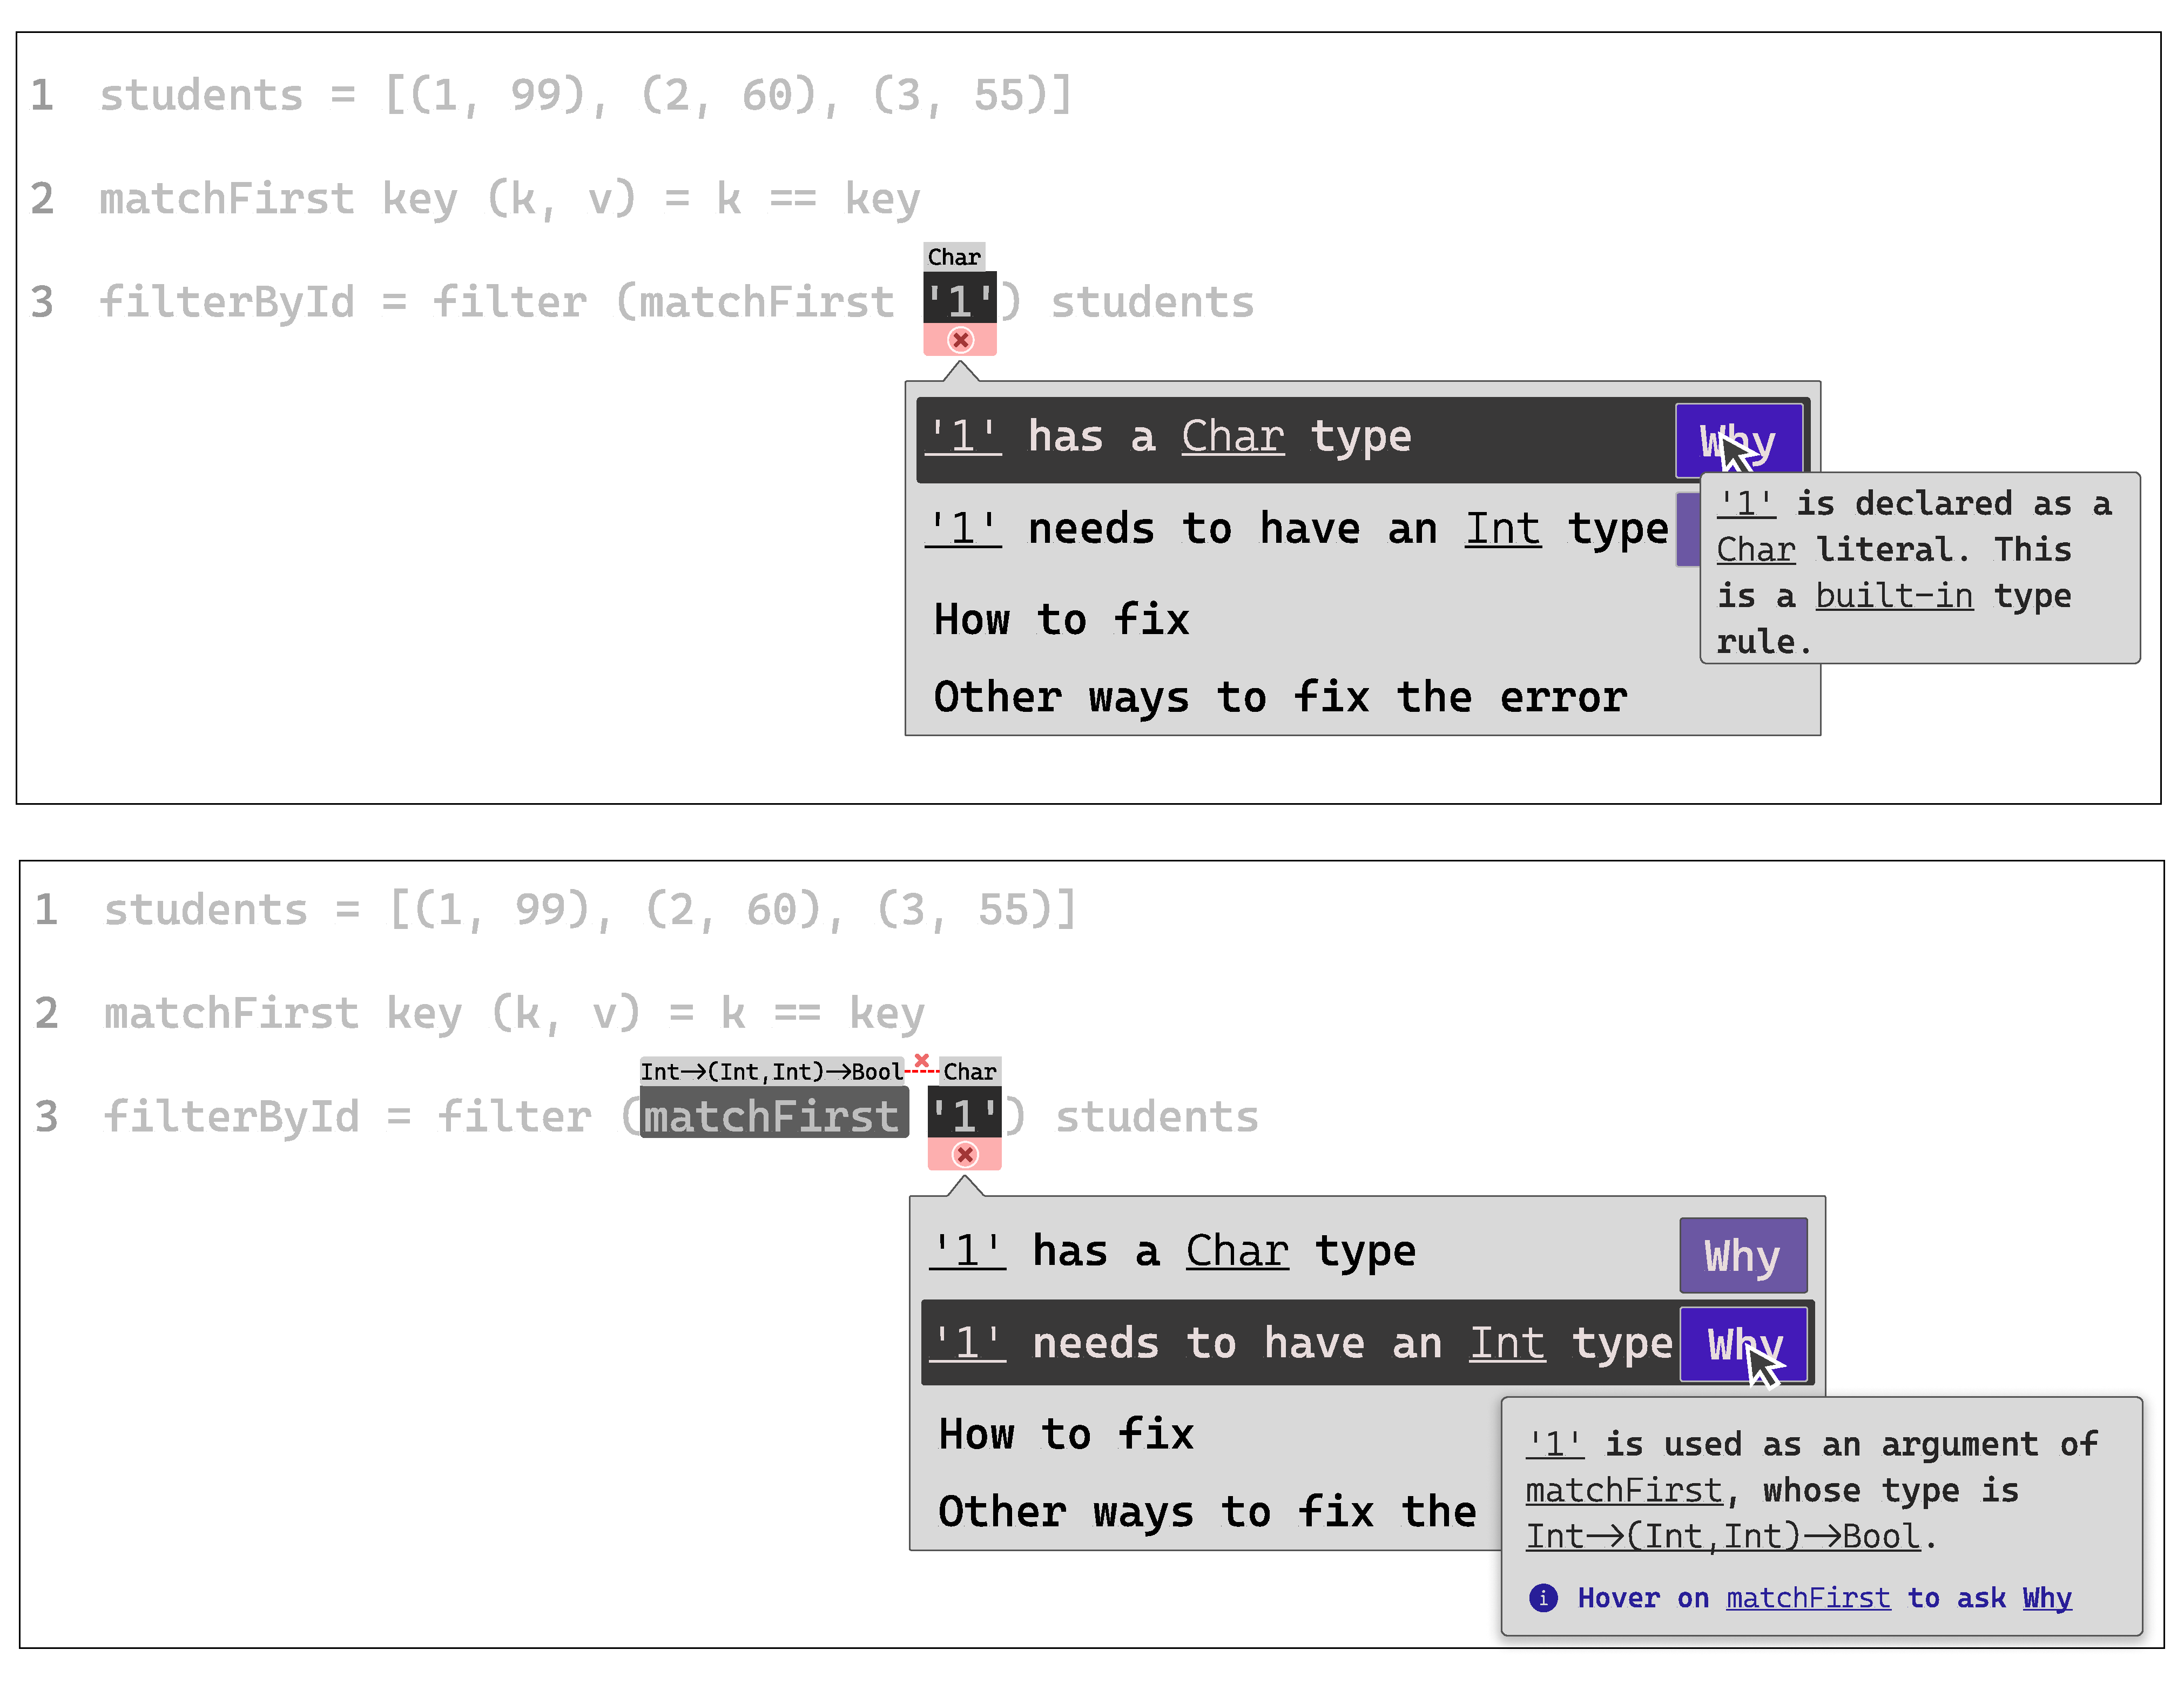
\includegraphics[width=\linewidth]{Why}
  \caption[An example of \textit{TypeTutor} providing explanation (`why' questions)]{
      \label{fig:why}
      The figure shows how \textit{TypeTutor} would provide programmers valid `why' questions to ask in a type error. When hovering on a location that is marked as a type error, \textit{TypeTutor} will identify an `expected' type (Top) and an `actual' type (Bottom). \textit{TypeTutor} would also prompt programmers to interrogate each branch to understand how these conclusions are drawn by hovering on the `Why' buttons. 
    }
\end{figure}



\subsubsection*{Follow-up questions}

In the context of debugging type errors, particularly multi-step type errors, it proves beneficial to enable programmers to incrementally uncover the underlying inference logic. \textit{TypeTutor} will support this process by allowing programmers to ask follow-up questions. Typically, these questions build upon the responses to earlier inquiries. Follow-up questions in \textit{TypeTutor} would facilitate tasks akin to the interactive debugging steps in \chameleon{}. However, unlike \chameleon{}, \textit{TypeTutor} would not need a separate interface for such a task. Instead, when a response includes the option for further inquiry, \textit{TypeTutor} would provide a follow-up hint at the end of the answer, encouraging programmers to continue tracing the root cause (Fig.~\ref{fig:follow-up}). This integrated approach would help maintain a streamlined user experience while enabling deep exploration of type errors.


\begin{figure}[hbt]
  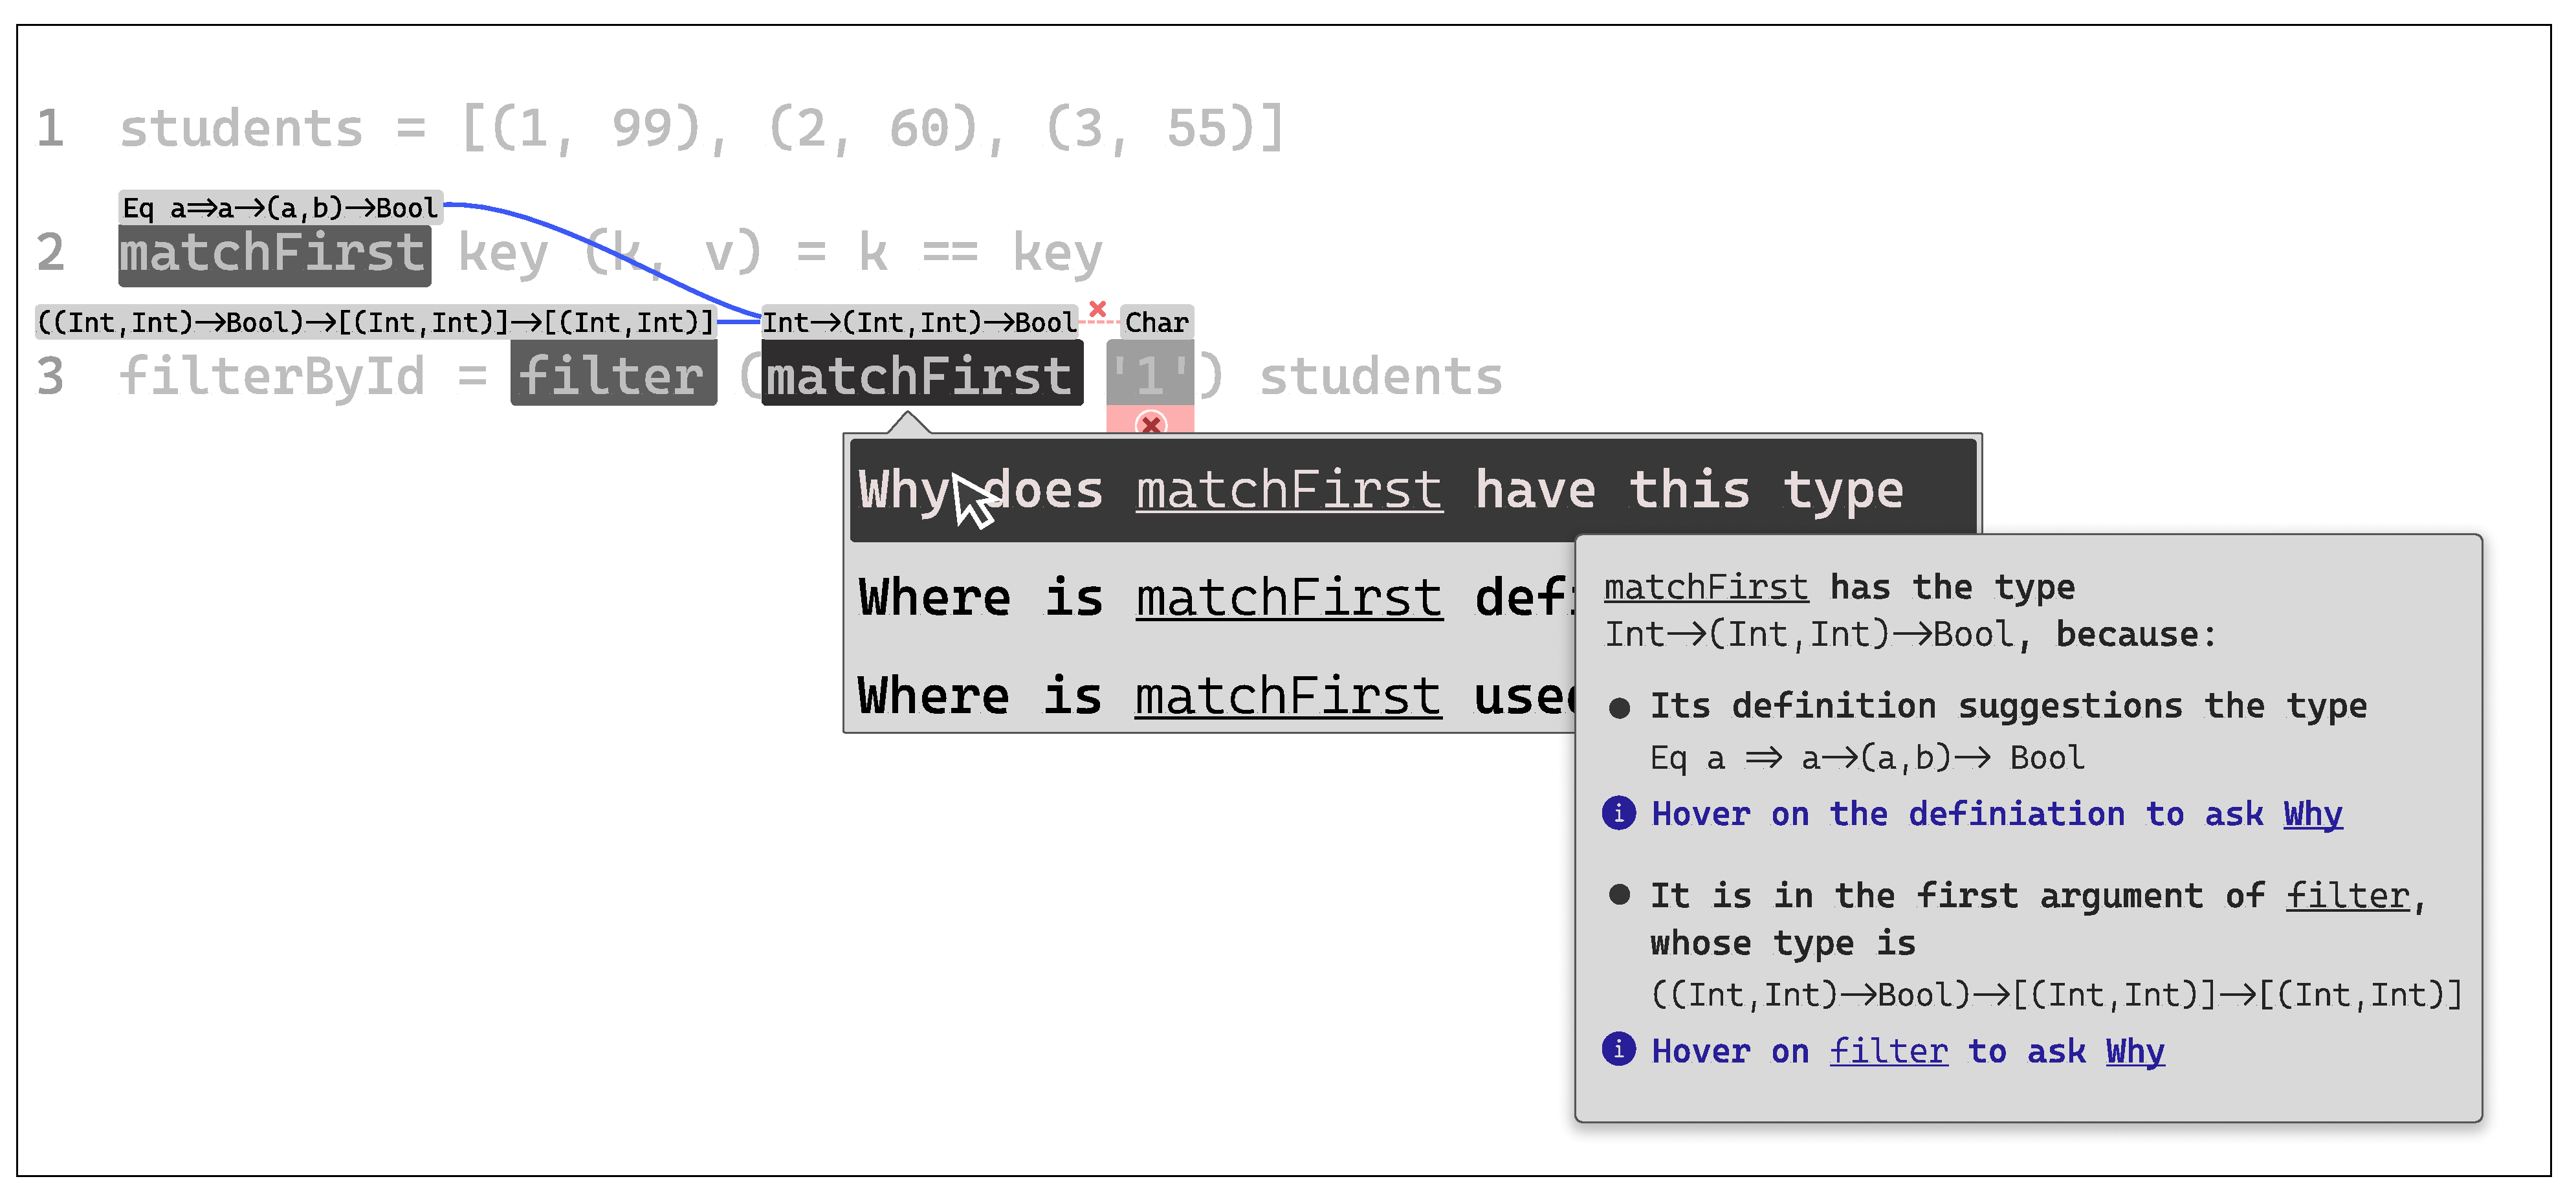
\includegraphics[width=\linewidth]{FollowUp}
  \caption[An example of \textit{TypeTutor} providing further explanation based on previous response (follow-up questions)]{
    \label{fig:follow-up}
     Following the case in Fig.~\ref{fig:why}, \textit{TypeTutor} will prompt programmers to ask follow-up questions. In this case, \textit{TypeTutor} will inform the programmer that \texttt{matchFirst} on line 3 has the type \texttt{Int -> (Int, Int) -> Bool} can be inferred from two pieces of clues:  the definition of \texttt{matchFirst} and the \texttt{filter} on line 3 instantiated as \texttt{((Int, Int) -> Bool) -> [(Int, Int)] -> [(Int, Int)]}. Programmers can trace further by following the hints again in the answer section.
    }
\end{figure}

\subsubsection*{How questions}

'How' questions in debugging focus on providing prescriptive guidance regarding program errors. Such questions do not solely depend on logical precision; they require understanding the knowledge gaps and delivering clear, followable instructions. \textit{TypeTutor} would aid programmers by facilitating questions on how to rectify specific type errors. In Goanna, the Maximal Satisfiable Subsets (MSS) analysis can suggest the recommended type for each possible correction. \textit{TypeTutor} would advance this concept by offering examples of syntax changes tailored to these recommended types. In the example (Fig.~\ref{fig:how}), \textit{TypeTutor} would provide various examples of how to change \texttt{'1'} to an Integer type, including changing it to an integer literal, an integer variable, or an expression that evaluates to an integer. 



\begin{figure}[hbt]
  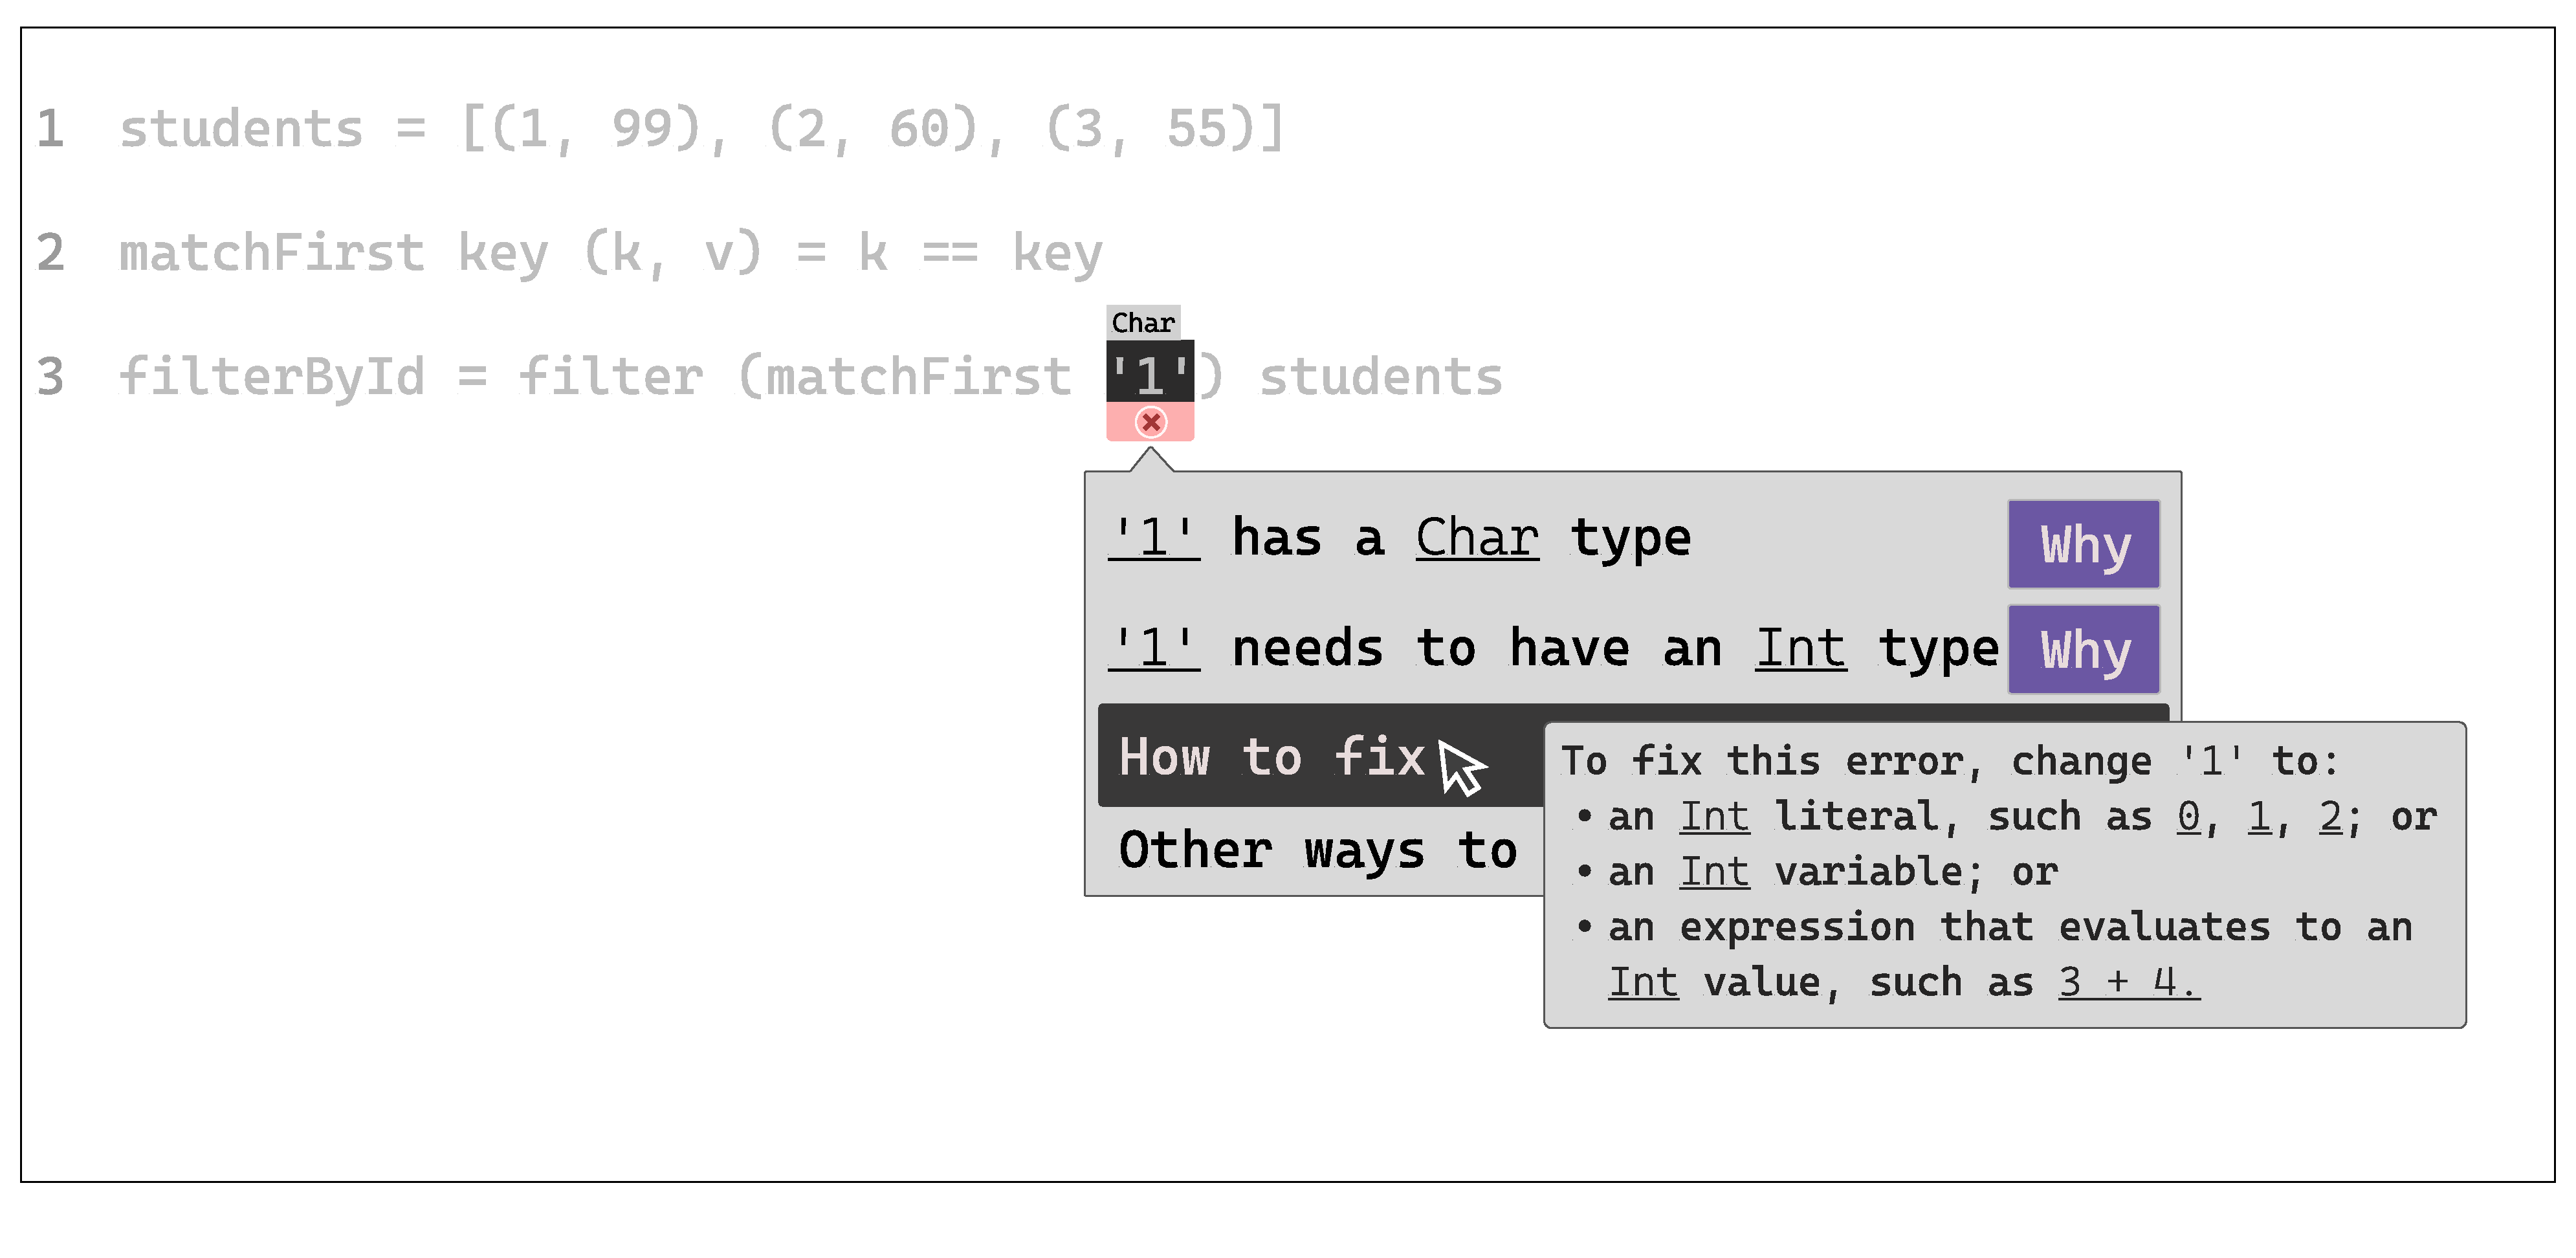
\includegraphics[width=\linewidth]{How}
  \caption[An example of \textit{TypeTutor} providing change suggestion (`how' questions)]{
    \label{fig:how}
    Following the case in Fig.~\ref{fig:why}, \textit{TypeTutor} will provide instructions on how to fix the type error. In detail,  \textit{TypeTutor} will provide various examples of how to change \texttt{'1'} to an Integer type, including changing it to an integer literal, an integer variable, or an expression that evaluates to an integer.
    }
\end{figure}

\subsubsection*{What-if questions}
Finally, as we have identified, type errors frequently involve multiple potential causes and explanations. When integrated into a question-and-answer interface, the presence of multiple causes naturally prompts counterfactual questions such as "What are other ways that can cause this type error?" Recognizing this, \textit{TypeTutor} will provide a natural and user-friendly interface for exploring various potential causes and solutions. This approach, while similar to the functionality offered by Goanna, features a more concise and intuitive interface for programmers to switch between different potential causes. With \textit{TypeTutor}, programmers will find the option: `Other ways to fix the error' in every type error question list; hovering over the option will present alternative explanations and resolution plans (Fig.~\ref{fig:what-if}).

\begin{figure}[hbt]
  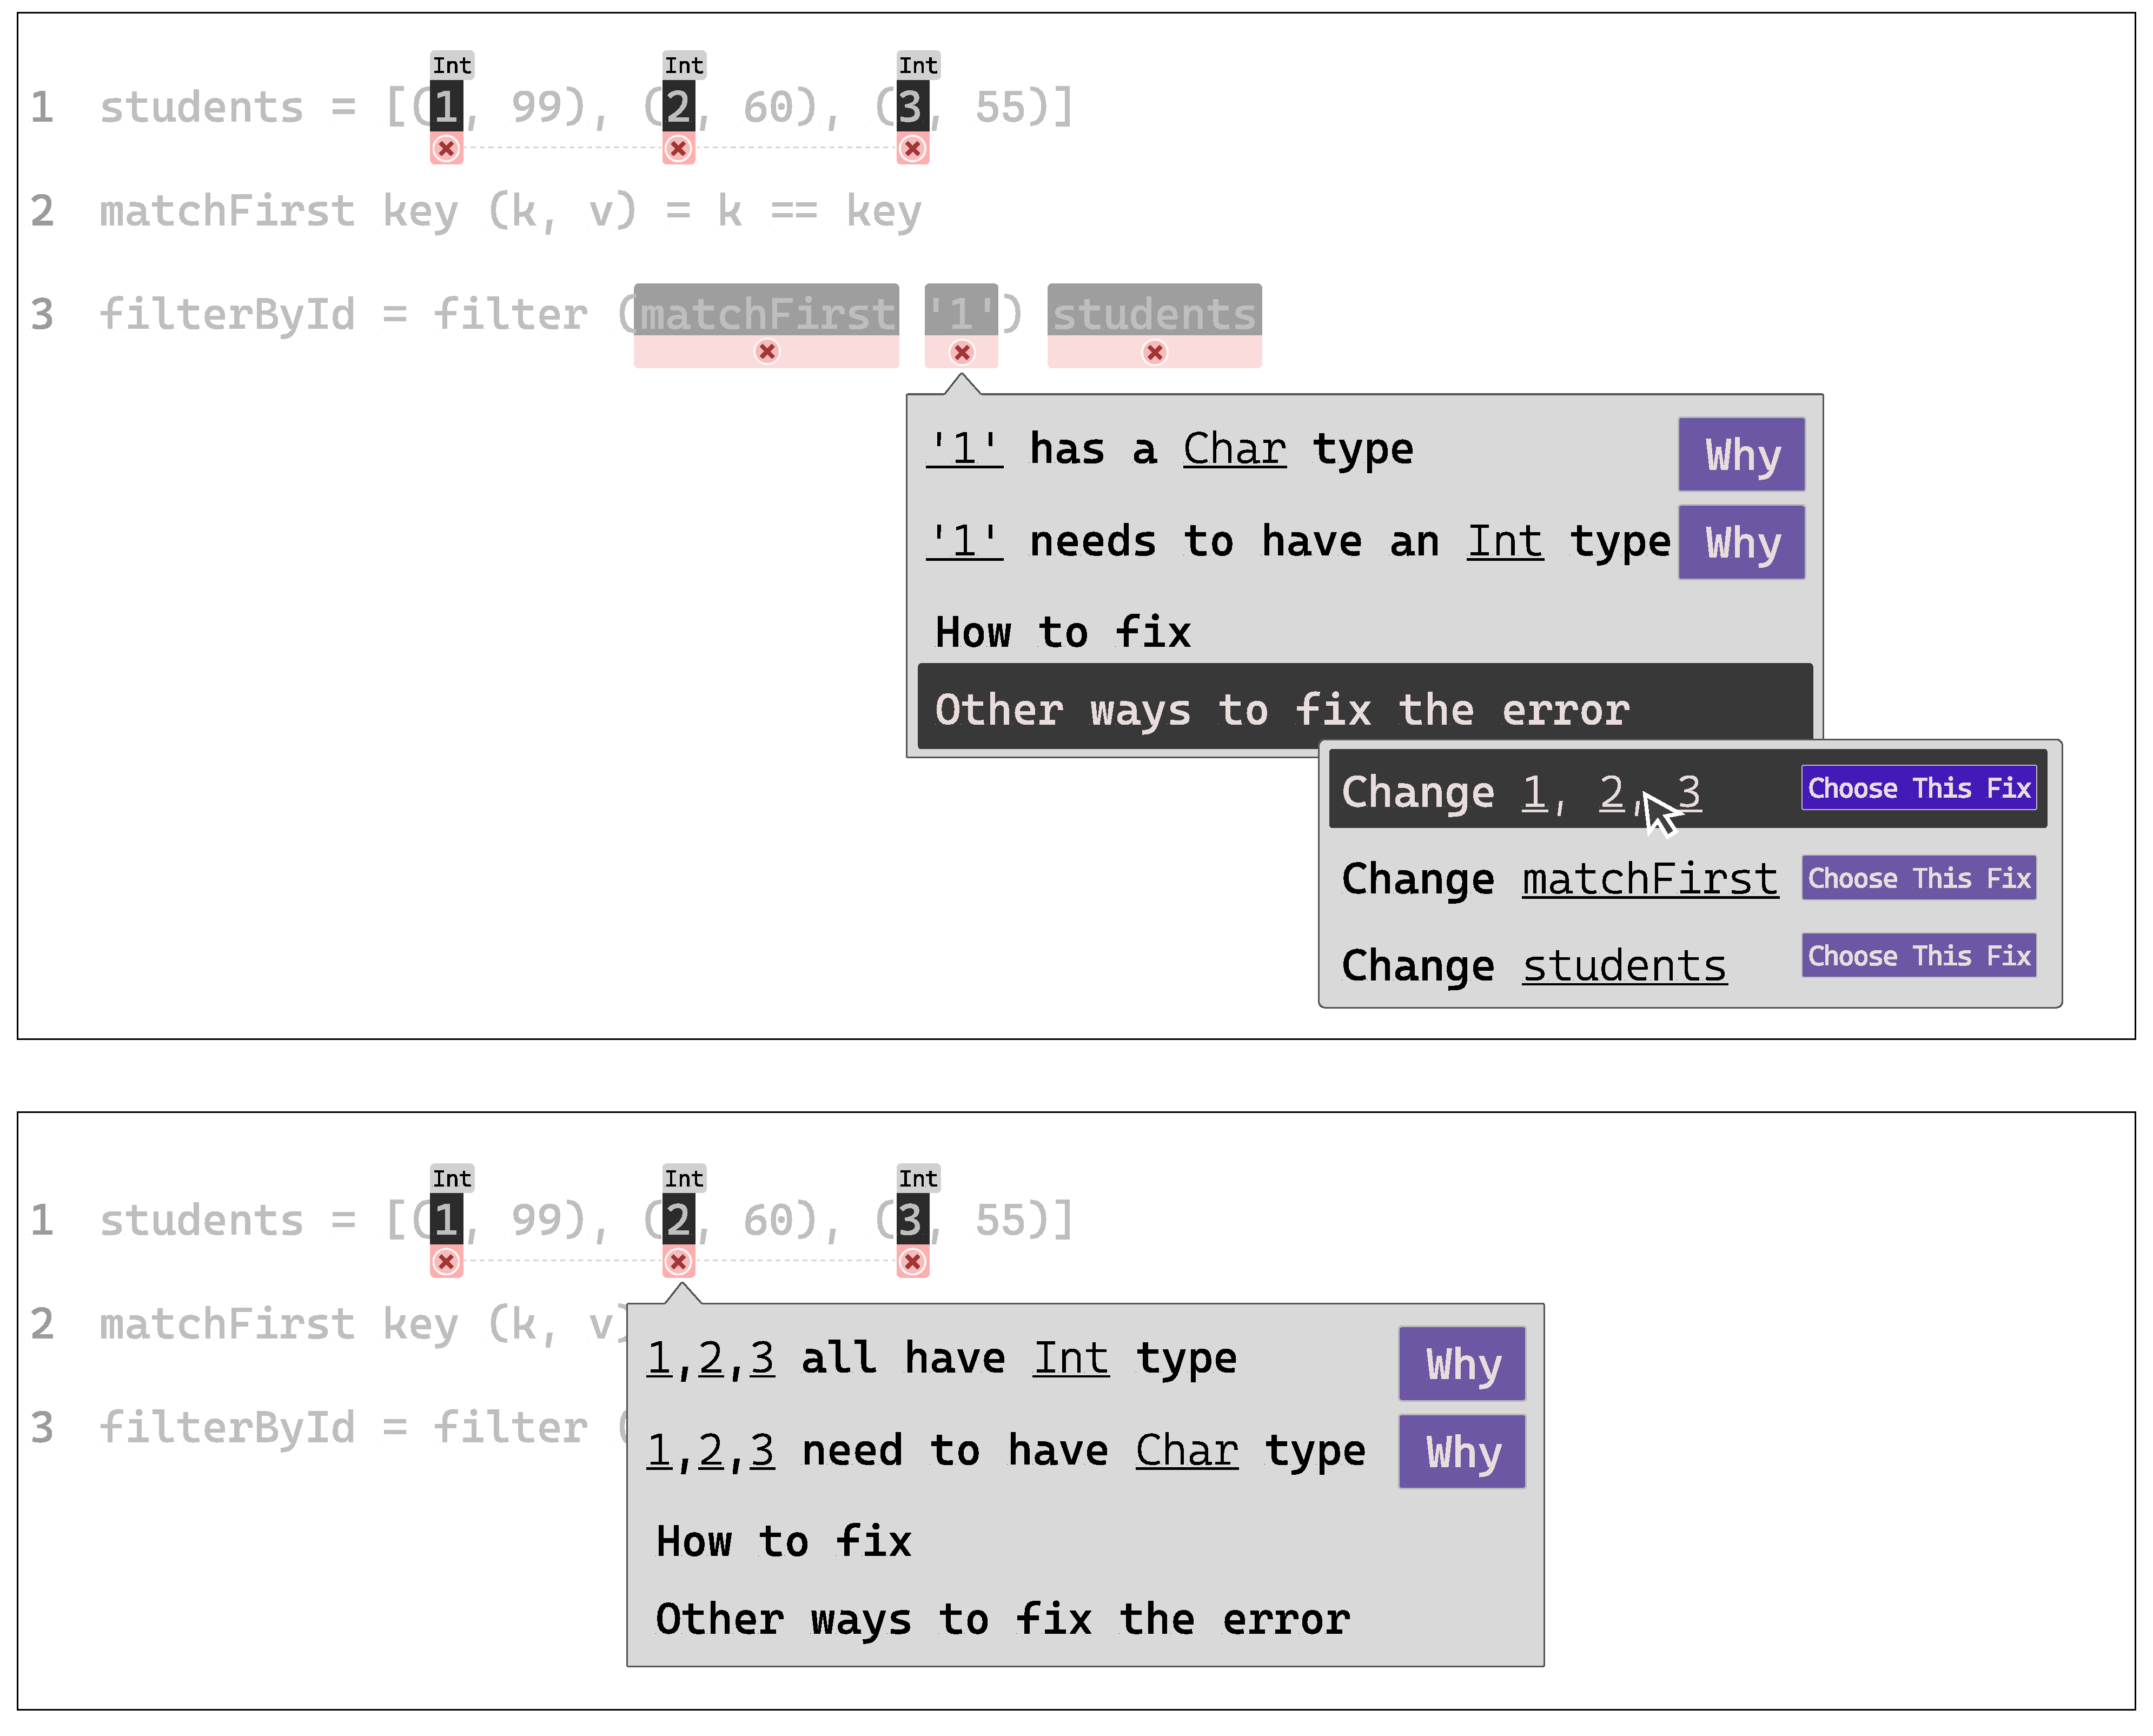
\includegraphics[width=\linewidth]{WhatIf}
  \caption[An examples of \textit{TypeTutor} addressing alternative causes (`what-if' questions)]{
      \label{fig:what-if}
      If the programmer disagrees that the literal \texttt{'1'} is the cause of the error and should be changed, \textit{TypeTutor} will provide alternative explanations and resolution plans. When hovering on the option `Other ways to fix the error', \textit{TypeTutor} will show three other potential fixes (Top). Choosing any of them, say the first option, will change the type error mark to another set of locations, and different explanations are provided when asking the `why' question at the new type error.
    }
\end{figure}


\subsection*{Integration with Large Language Models}
At the time of writing this thesis, LLMs were actively experimented with performing all kinds of tasks that require human creativity, including programming. Many attempts have been made to use LLMs in programming tasks \cite{Shi2024-bj}, intending to free programmers for higher-level thinking. This development is tangential to our objective of explaining type errors and reasoning about the logic of type inference. 

\begin{figure}[hbt]
  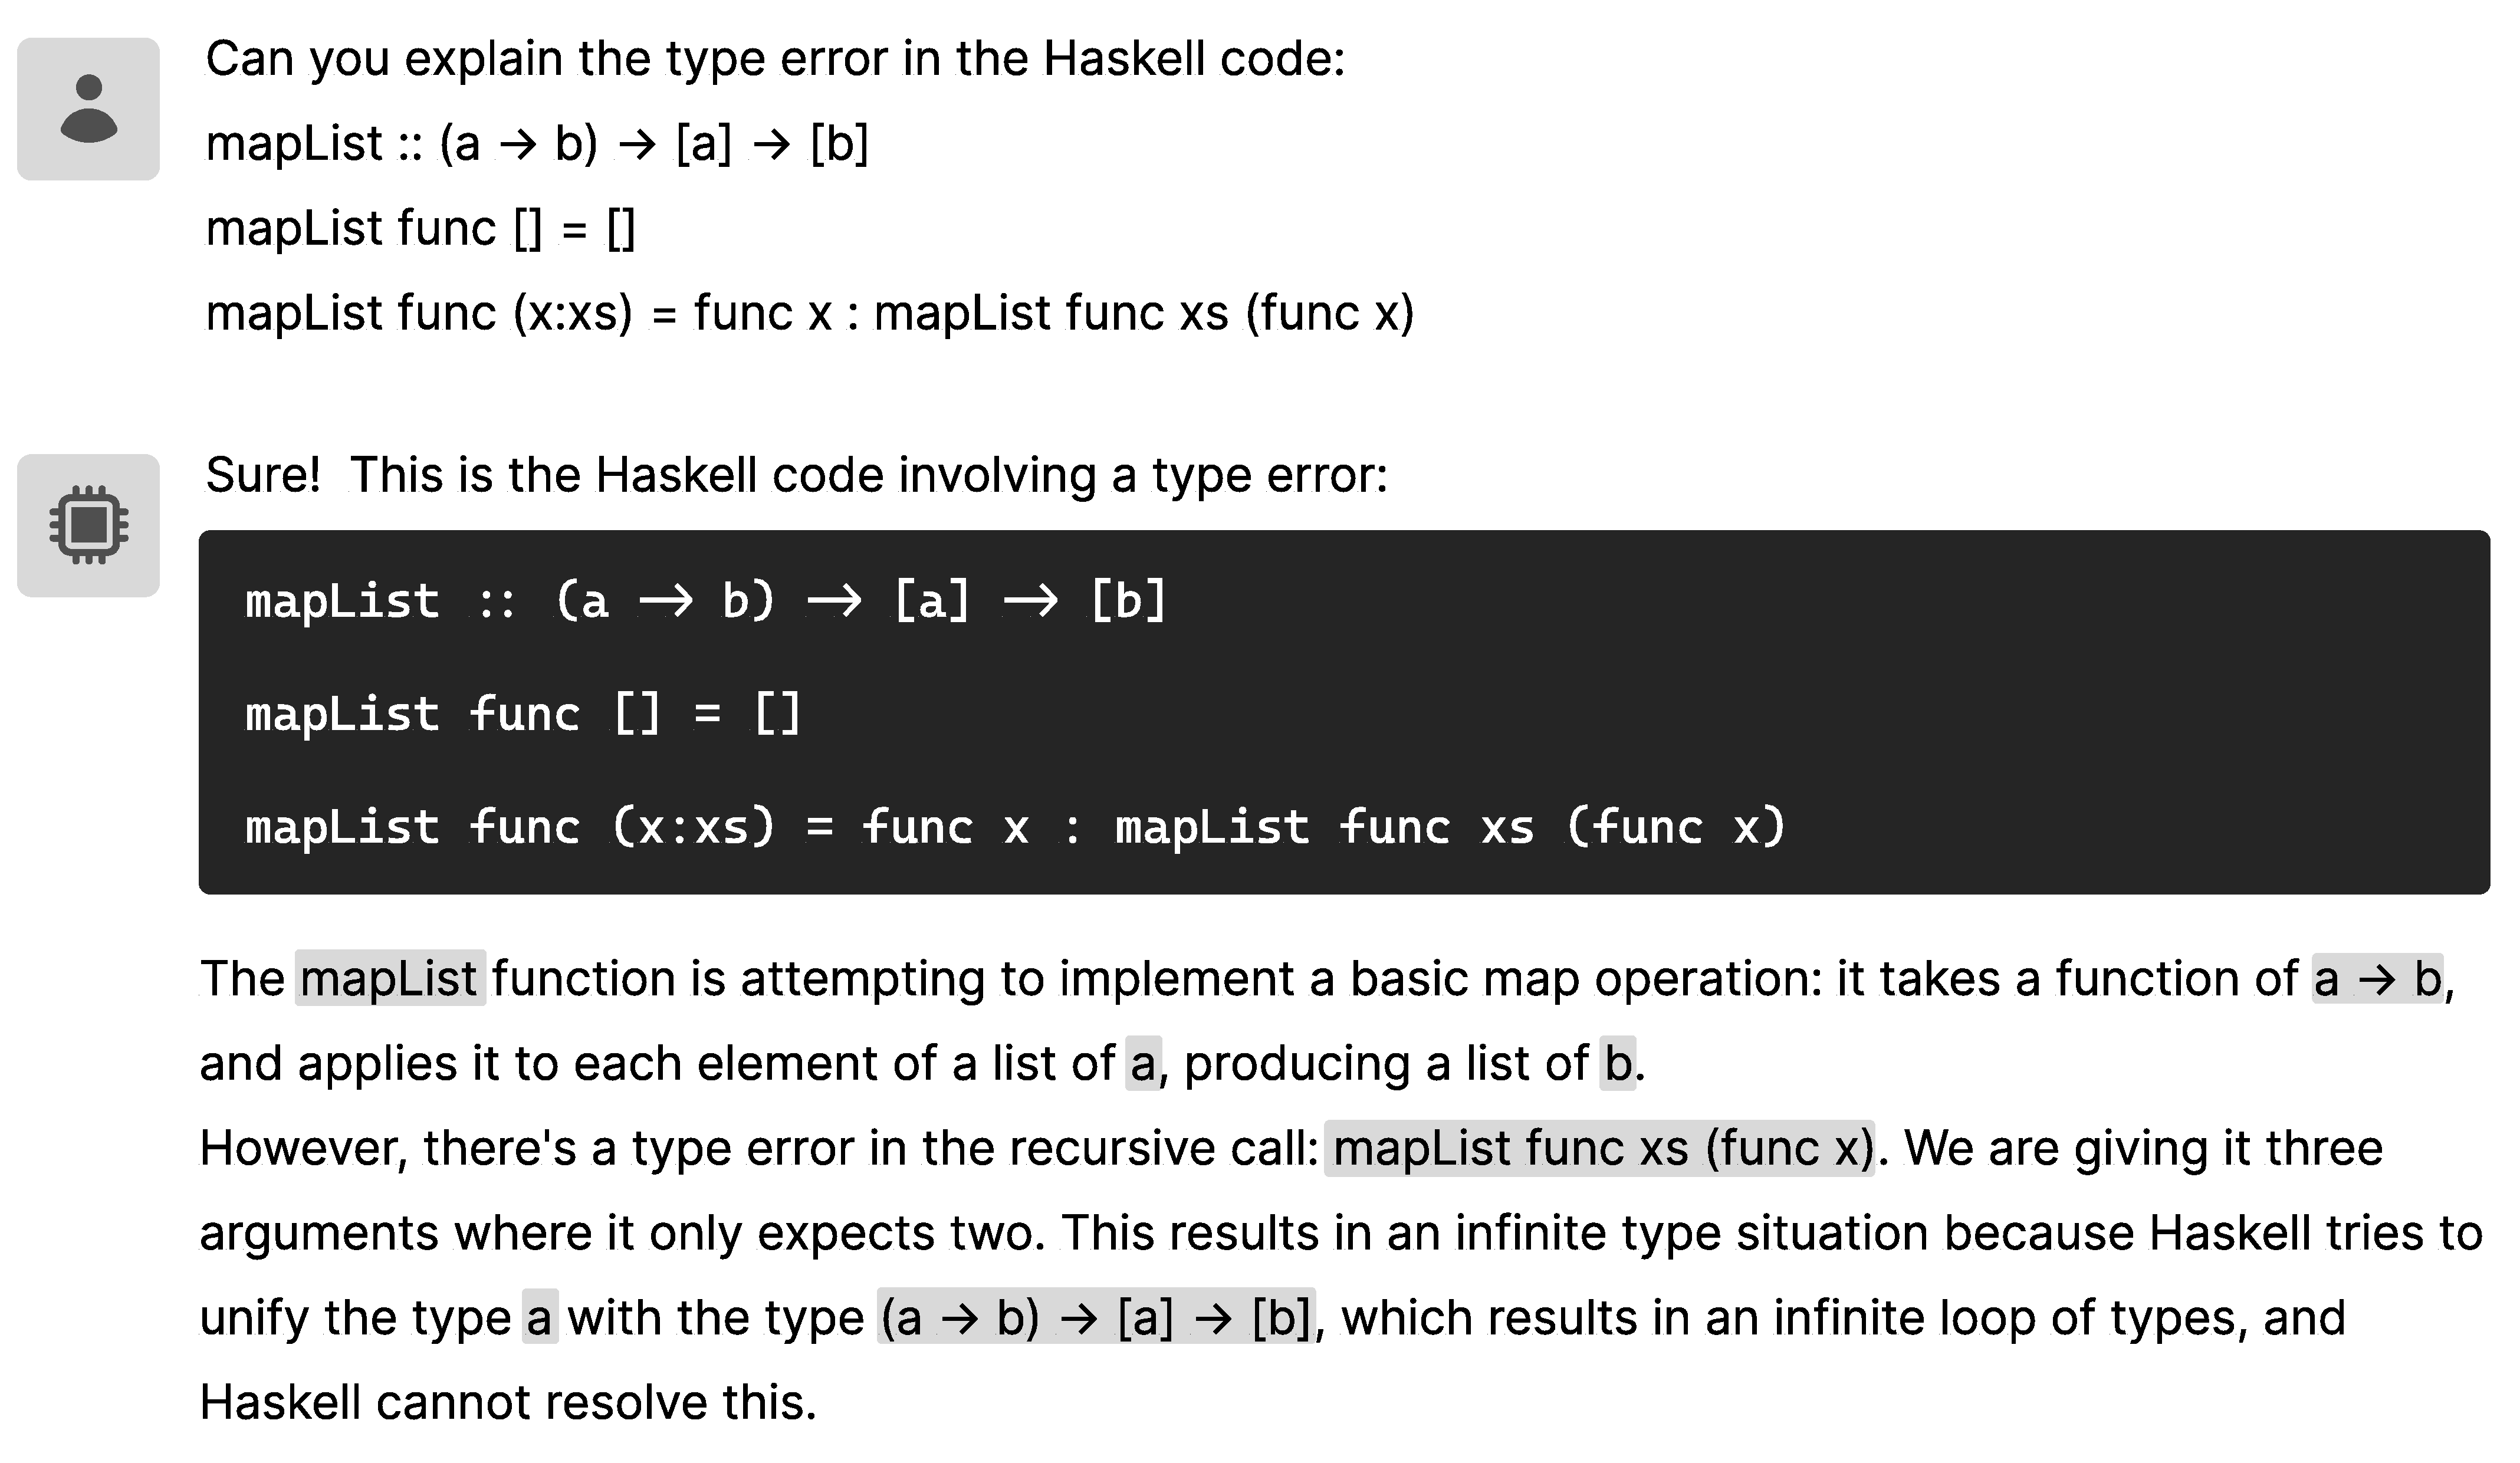
\includegraphics[width=\linewidth]{LLM}
  \caption[LLM explaining a type error; it began very accurate, then went on to give incorrect and contradicting analysis]{\label{fig:llm}
  The figure shows the user prompted LLM to explain the type error in a Haskell function definition \texttt{mapList}. LLM, at first, showed a profound understanding of the subject matter, clearly explained the intention of the function, and accurately identified the error location. In the last sentence, LLM claimed the definition would result in an infinite type because trying to unify \texttt{a} with \texttt{(a -> b) -> [a] -> [b]}. In reality, unifying two functions with different numbers of arguments will not cause infinite types. 
    }
\end{figure}

While LLMs have shown capability in recognizing basic errors, they often display a limited understanding of type theories and multi-step reasoning ability. Fig.~\ref{fig:llm} depicts a type error caused by mismatching numbers of arguments in the function \texttt{mapList}; although provided a correct error identification at the start, GPT 4 proceeded to claim, “This results in an infinite type situation because Haskell tries to unify the type \texttt{a} with the type \texttt{(a -> b) -> [a] -> [b]}, which results in an infinite loop of types, and Haskell cannot resolve this,” illustrating a fundamental lack of understanding of type theory.

\begin{figure}[hbt]
  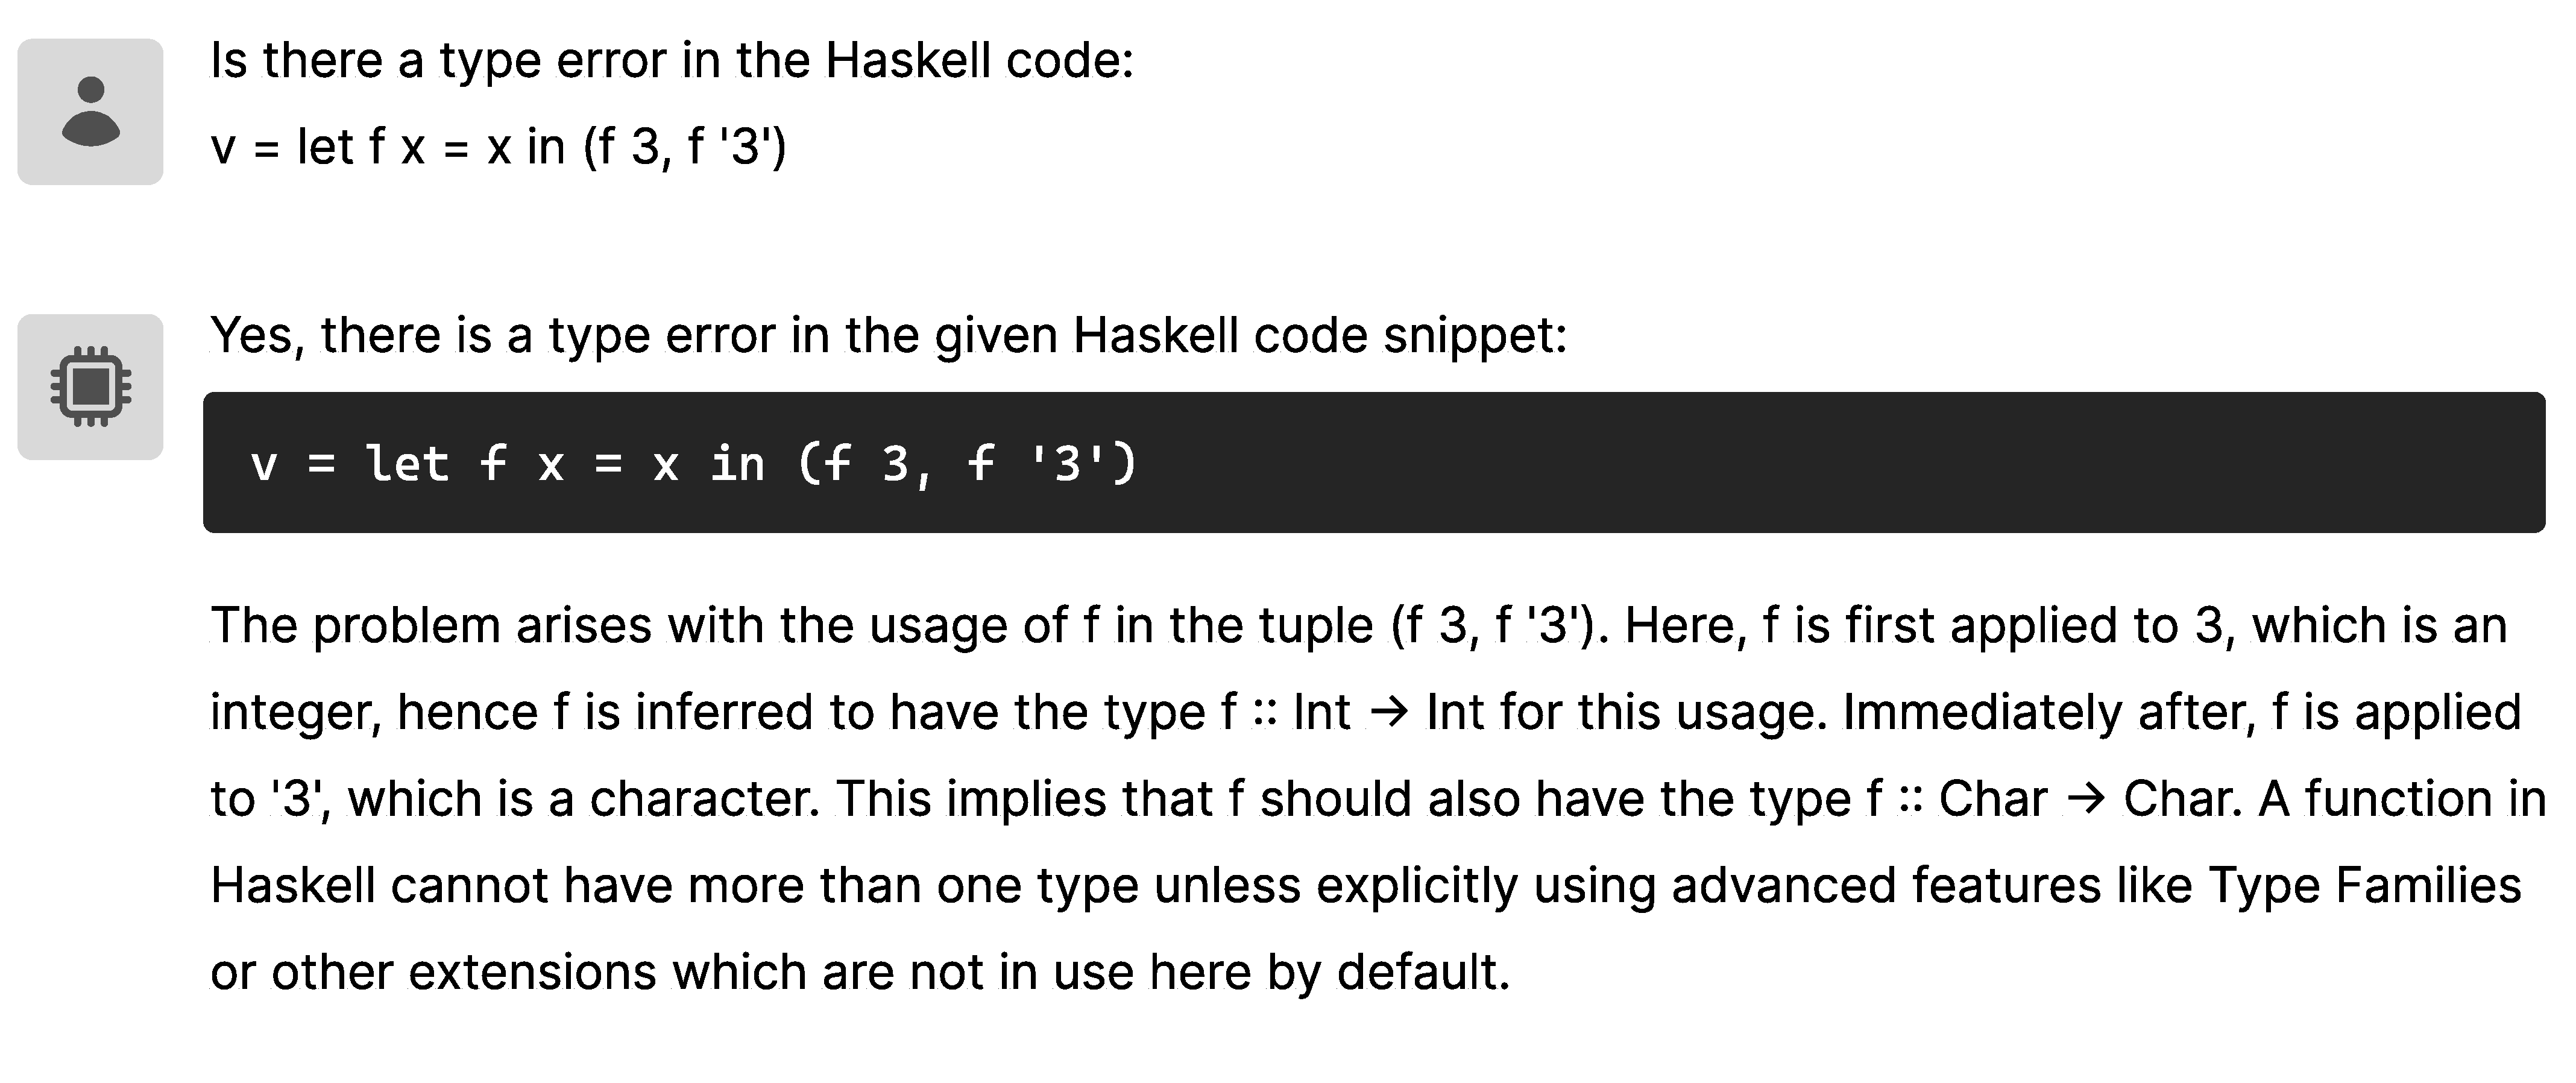
\includegraphics[width=\linewidth]{LLM2}
  \caption[An example where LLM identified a type error in well-typed source code]{\label{fig:llm2}
  The figure shows a user asking an LLM whether the provided Haskell source code has a type error. While the provided code is, in fact, well-typed, LLM hallucinated a type error and ignored how polymorphic functions work in Haskell. In the example, the function \texttt{f},  defined the same way as the \texttt{id} function, can be applied with a value of any type.
    } 
\end{figure}

When tested with the prompt "Is there a type error in the Haskell code: v = let f x = x in (f 3, f '3')", most LLMs incorrectly reported yes (Fig.~\ref{fig:llm2}). However, this Haskell code is indeed well-typed. LLMs can give wrong explanations and find type errors that do not exist, unlike tools like GHC, Helium, and Goanna. While there is clearly a role for their usage in programming assistance \cite{Lee2024-hs}, they do not “reason” about types and, hence, are not trustworthy.

While LLMs are getting more and more accurate with each iteration, some doubt whether they will never become as reliable as theory-based tools \cite{Berglund2023-ig}. We believe in the great potential of integrating LLMs with existing theory-based tools, such as \chameleon{} and Goanna. This integration could enhance the performance of LLMs by aligning their operations with accurate theoretical guides or utilizing their strengths in areas where traditional tools fall short, such as suggesting syntactical improvements. This synergy could lead to more robust programming assistance using both types of tools. We propose two candidate workflows:

\itemize{
  \item{\textbf{Code Generation and Validation}: LLMs could generate initial source code based on user provided propmts.  Theory-based tools, such as \chameleon{} and Goanna, then check for errors. Detected errors could be fed back to the LLMs for corrections, enhancing both the efficiency and accuracy of code development.}
  \item {\textbf{Error Tutoring and Resolution}: Theory-based tools could identify errors in manually written code, with LLMs suggesting syntax corrections. This combines the precise error detection from traditional theory-based tools with the ability of LLMs to generate effective syntax changes, surpassing traditional tools in this domain.}
}

\subsection*{Support for Other Languages}
Haskell serves as a vital platform for the experiments of programming languages and type systems. We firmly believe that the next critical phase in our research involves expanding our tools to encompass other languages. Recently, we observed that the challenges of overcoming complex type errors have permeated several mainstream languages, including Rust \cite{Zeng2019-ou} and TypeScript \cite{Scarsbrook2023-uq}. By integrating our debugging tools into these languages, we would be able to engage a broader audience and subject our tools to a diverse range of software projects varying in style and scale. This will not only increase the applicability of our tools, but also provide us with extensive insights into how to further improve our design.

Much of our work has already been conceived with the adaptability to multiple languages in mind. For example, GeckoGraph is designed to be language-agnostic, allowing for implementations in different programming languages. However, adapting tools like \chameleon{} and Goanna presents certain complexities. Although the analysis of unsatisfiable constraints and the theories and implementations concerning the enumeration of Minimal Unsatisfiable Subsets (MUSes) and Minimal Correction Subsets (MCSes) are universally applicable across all languages, specific challenges arise when taking into account the nuances of individual languages.

The first challenge involves constraint generation. Each language requires the development of specific rules for generating constraints and conforming to its own typing rules, which could necessitate substantial modifications depending on the type-level features each language possesses. For instance, all functions in Haskell are curried, meaning that they can be provided with fewer arguments than they are defined, a characteristic absent in TypeScript, where functions are defined with fixed arity and can be overloaded. This discrepancy means that in TypeScript, a type error can occur if a function is applied to fewer arguments than it is defined for, an error that would not typically arise in Haskell.

The second challenge concerns the presentation of type errors, which may need nuanced adjustments for different languages. For example, novel visualization techniques may be required to effectively convey concepts absent in Haskell, such as row polymorphism in TypeScript or lifetime constraints in Rust. By addressing these challenges, we can truly leverage the potential of our tools across various programming environments.

\subsubsection*{Supporting Dependently Typed Languages}

As mentioned in previous chapters, dependently typed languages like Idris and Agda represent a rigorous subclass within the realm of statically typed languages. These languages uniquely enable the type-level computation of values and types, allowing programmers to embed fine-grained and precise constraints to ensure program correctness at compile time. Due to their ability to directly encode program behavior into types, programs written in dependently typed languages can often be validated purely through the type-checking process. This makes them ideal candidates for code generation through LLMs, where programmers can perform checks on whether they conform to the provided specifications. 

However, despite their potential, dependently typed languages currently hold a modest position in the mainstream programming landscape. We believe that enhancing our type debugging tools to support dependently typed languages can bring a step forward in improving their learnability and adoption, especially among programmers who are new to dependent typing. As type-level computations grow in complexity, our tools, designed to aid in understanding and reasoning, become increasingly valuable. 


\section{Conclusion}


The field of programming languages is truly captivating, representing a confluence of ideas from various disciplines and schools of thought. Among the myriad concepts, functional programming and static typing are particularly important for their profound impact on the domain. My research aims to highlight the benefits of functional programming and static typing while also addressing the challenges they pose. By refining how types and type errors are presented and explained, we strive to make functional programming and static typing accessible and user-friendly to programmers.

Our methodologies are largely grounded in theories of constraint satisfiability. These include analyzing Minimal Unsatisfiable Subsets (MUS) through tools like \chameleon{} and Minimal Correction Subsets (MCS) via Goanna. In addition, we employ various human-centered research techniques, such as formative studies, user studies, and rapid prototyping. These approaches not only enhance the practicality of our research, but also its relevance to real-world programming.

We are convinced that type error enhancement and explanation is a valuable trajectory for research in programming languages. It is our hope that our work will serve as a useful reference, inspiring future studies that continue to augment and expand our arsenal of type error debugging tools.




%----------------------------------------------------------------------------------------
%	THESIS CONTENT - APPENDICES
%----------------------------------------------------------------------------------------

\appendix % Cue to tell LaTeX that the following "chapters" are Appendices

% Include the appendices of the thesis as separate files from the Appendices folder
% Uncomment the lines as you write the Appendices

%% Appendix A

\chapter{Game Levels In User Study ZeroToHero} % Main appendix title

\label{levels} % For referencing this appendix elsewhere, use \ref{AppendixA}


We provide all the level settings we used in our user study. The online game is still open source and available for evaluation \cite{Anonymous_undated-ne}. However, this can be attempted locally with a Haskell interpreter or even with a pen and paper. The target type is the desired type signature for the function \texttt{zeroToHero}. The available functions show a list of functions that are allowed to be used in the implementation. It is not required to use all the available functions, and it is not forbidden to use any other functions or variables outside the provided functions; even the Haskell prelude is not available. 


\section{Level 1: Trial run}

\subsection{Target Type } 
\begin{itemize}
    \item \texttt{zeroToHero :: Zero a -> Hero a}
\end{itemize}

\subsection{Available Functions} 
\begin{itemize}
    \item \texttt{f :: Zero a -> Hero a}
\end{itemize}

\subsection{Possible Solution} 
\begin{itemize}
    \item \texttt{zeroToHero z = f z}
\end{itemize}


\section{Level 2: Assemble required}

\subsection{Target Type} 
\begin{itemize}
    \item \texttt{zeroToHero :: Zero a -> Hero a}
\end{itemize}

\subsection{Available Functions} 
\begin{itemize}
    \item \texttt{runZero :: Zero a -> a}
    \item \texttt{mkHero :: a -> Hero a}
    \item \texttt{(\$) :: (a -> b) -> a -> b}
\end{itemize}

\subsection{Possible Solution} 
\begin{itemize}
    \item \texttt{zeroToHero z = mkHero (runZero z)}
\end{itemize}

\section{Level 3: Which path?}
\subsection{Target Type } 
\begin{itemize}
    \item \texttt{zeroToHero :: Zero a -> Hero (a, a)}
\end{itemize}

\subsection{Available Functions} 
\begin{itemize}
    \item \texttt{f1 :: Zero a -> Hero a}
    \item \texttt{f2 :: Zero a -> (a, a)}
    \item \texttt{f3 :: Hero a -> Hero (a, a)}
    \item \texttt{(\$) :: (a -> b) -> a -> b}
    \item \texttt{(.) :: (b -> c) -> (a -> b) -> a -> c}
\end{itemize}

\subsection{Possible Solution} 
\begin{itemize}
    \item \texttt{zeroToHero z = f3 . f1 \$ z}
\end{itemize}


\section{Level 4: A repeating pattern}
\subsection{Target Type } 
\begin{itemize}
    \item \texttt{zeroToHero :: Zero a b -> Hero b b}
\end{itemize}

\subsection{Available Functions} 
\begin{itemize}
    \item \texttt{f1 :: Zero a b -> Hero b a}
    \item \texttt{f2 :: Zero a a -> Hero a a}
    \item \texttt{f3 :: Zero a b -> Zero b a}
    \item \texttt{f4 :: Zero a b -> Zero b b}
    \item \texttt{(\$) :: (a -> b) -> a -> b}
    \item \texttt{(.) :: (b -> c) -> (a -> b) -> a -> c}
\end{itemize}

\subsection{Possible Solution} 
\begin{itemize}
    \item \texttt{zeroToHero z = f2 . f4 \$ z}
\end{itemize}


\section{Level 5: A perfect pair}
\subsection{Target Type } 
\begin{itemize}
    \item \texttt{zeroToHero :: Zero a b -> Hero b b}
\end{itemize}

\subsection{Available Functions} 
\begin{itemize}
    \item \texttt{fst :: (a, b) -> a}
    \item \texttt{snd :: (a, b) -> b}
    \item \texttt{f1 :: Zero a b -> Hero b a}
    \item \texttt{f2 :: Zero a a -> Hero a a}
    \item \texttt{f3 :: Zero a b -> Zero b a}
    \item \texttt{f4 :: Zero a b -> Zero b b}
    \item \texttt{(\$) :: (a -> b) -> a -> b}
    \item \texttt{(.) :: (b -> c) -> (a -> b) -> a -> c}
\end{itemize}

\subsection{Possible Solution} 
\begin{itemize}
    \item \texttt{zeroToHero z = snd .f3 . f1 \$ z}
\end{itemize}


\section{Level 6: Monty Hall}
\subsection{Target Type } 
\begin{itemize}
    \item \texttt{zeroToHero :: Zero a b c -> Hero c a}
\end{itemize}

\subsection{Available Functions} 
\begin{itemize}
    \item \texttt{f1 :: Zero a b c-> Zero c b a}
    \item \texttt{f2 :: Zero a b c -> Zero a c c}
    \item \texttt{f3 :: Zero a b c -> Hero b c}
    \item \texttt{(\$) :: (a -> b) -> a -> b}
    \item \texttt{(.) :: (b -> c) -> (a -> b) -> a -> c}
\end{itemize}

\subsection{Possible Solution} 
\begin{itemize}
    \item \texttt{zeroToHero z = f3 . f1 . f2 \$ z}
\end{itemize}

\section{Level 7: TIE fighter}
\subsection{Target Type } 
\begin{itemize}
    \item \texttt{zeroToHero :: Zero a b c -> Hero c}
\end{itemize}

\subsection{Available Functions} 
\begin{itemize}
    \item \texttt{f1 :: Zero a b c -> Hero (a -> b)}
    \item \texttt{f2 :: Zero a b c -> Hero (b -> c)}
    \item \texttt{f3 :: Zero a b c -> Hero a}
    \item \texttt{(<\$>) :: (a -> b) -> Hero a -> Hero b}
    \item \texttt{(<*>) :: Hero (a -> c) -> Hero a -> Hero c}
    \item \texttt{(\$) :: (a -> b) -> a -> b}
    \item \texttt{(.) :: (b -> c) -> (a -> b) -> a -> c}
\end{itemize}

\subsection{Possible Solution} 
\begin{itemize}
    \item \texttt{zeroToHero z = f2 z <*> (f1 z <*> f3 z)}
\end{itemize}

\section{Level 8: The middle man}
\subsection{Target Type } 
\begin{itemize}
    \item \texttt{zeroToHero :: (a -> d) -> (b -> d) -> (c -> d) -> Zero a b c ->  Hero a d c}
\end{itemize}

\subsection{Available Functions} 
\begin{itemize}
    \item \texttt{f1 :: Zero a b c -> Zero c a b}
    \item \texttt{f2 :: Zero a b c -> Hero a b c}
    \item \texttt{fmap :: (c -> d) -> Zero a b c -> Zero a b d}
    \item \texttt{(\$) :: (a -> b) -> a -> b}
    \item \texttt{(.) :: (b -> c) -> (a -> b) -> a -> c}
\end{itemize}

\subsection{Possible Solution} 
\begin{itemize}
    \item \texttt{zeroToHero ad bd cd z = f2  . f1  . f1  . fmap bd  . f1 \$ z}
\end{itemize}

\section{Level 9: Split the difference}
\subsection{Target Type } 
\begin{itemize}
    \item \texttt{zeroToHero :: Zero a b c d ->  Hero d d d d}
\end{itemize}

\subsection{Available Functions} 
\begin{itemize}
    \item \texttt{f1 :: Zero a b c -> Zero c a b}
    \item \texttt{f2 :: Zero a b c -> Hero a b c}
    \item \texttt{fmap :: (c -> d) -> Zero a b c -> Zero a b d}
    \item \texttt{(\$) :: (a -> b) -> a -> b}
    \item \texttt{(.) :: (b -> c) -> (a -> b) -> a -> c}
\end{itemize}

\subsection{Possible Solution} 
\begin{itemize}
    \item \texttt{zeroToHero ad bd cd z = f2 \$ f1 \$ f1 \$ f3 \$ z}
\end{itemize}


\section{Level 10: The roller coaster}
\subsection{Target Type } 
\begin{itemize}
    \item \texttt{zeroToHero :: Zero (a -> b -> c -> d) a b c  -> Hero d}
\end{itemize}

\subsection{Available Functions} 
\begin{itemize}
    \item \texttt{f1 :: Zero (a -> b) a c d -> Zero () b c d}
    \item \texttt{f2 :: Zero a b c d -> Zero b c d a}
    \item \texttt{f3 :: Zero a b c d -> Hero d}
    \item \texttt{(\$) :: (a -> b) -> a -> b}
    \item \texttt{(.) :: (b -> c) -> (a -> b) -> a -> c}
\end{itemize}

\subsection{Possible Solution} 
\begin{itemize}
    \item \texttt{zeroToHero z = f3 . f2 . f2 . f1 . f2 . f1 . f2 . f1 \$ z}
\end{itemize}
%\include{Appendices/AppendixB}
%\include{Appendices/AppendixC}

%----------------------------------------------------------------------------------------
%	BIBLIOGRAPHY
%----------------------------------------------------------------------------------------

\printbibliography[heading=bibintoc]

%----------------------------------------------------------------------------------------

\end{document}  
